
\documentclass[11pt,spanish,
		listoftables,listoffigures]
		{tfgplantilla}


\usepackage[utf8]{inputenc} 

\usepackage{lipsum}

\usepackage{wrapfig}

\usepackage{float}

\usepackage{lscape}

\usepackage{pdfpages}

\title{\MakeUppercase{Desarrollo de una aplicación móvil} \\
	\MakeUppercase{para el tratamiento de las} \\
         \MakeUppercase{Enfermedades Cardiovasculares}}
\author{Ricardo Cajigas Arenas \\ José Ángel Sánchez Martín}
\tutor{José Ignacio Hidalgo Pérez}
\curs{Junio 2017}


\keywords{Enfermedades cardiovasculares, Aplicación móvil, Diabetes, Colesterol, Tabaquismo, Obesidad, Hipertensión Arterial, Riesgo Cardiovascular}              % Palabras clave
     	      {Cardiovascular Diseases, Mobile Application, Diabetes, Cholesterol, Smoking, Obesity, Arterial Hypertension, Cardiovascular Risk}        			  % Key words

\begin{document}

%%%%%%%%%%%%%%%%%%%%%%%%%%%%%%%%%%%%%%%%%%%%%%%%%%%%%%%%%%%%%%%%%%%%%%%%%%%%%%%%%%%%%%%%%%%%%%%%%%%%%%%%%%%%%%%%%%%%%%%%%
%																	     AUTORIZACIÓN DE DIFUSIÓN		                       															  %
%%%%%%%%%%%%%%%%%%%%%%%%%%%%%%%%%%%%%%%%%%%%%%%%%%%%%%%%%%%%%%%%%%%%%%%%%%%%%%%%%%%%%%%%%%%%%%%%%%%%%%%%%%%%%%%%%%%%%%%%%
%\chapter{Autorización de difusión}
%\cleardoublepage


%%%%%%%%%%%%%%%%%%%%%%%%%%%%%%%%%%%%%%%%%%%%%%%%%%%%%%%%%%%%%%%%%%%%%%%%%%%%%%%%%%%%%%%%%%%%%%%%%%%%%%%%%%%%%%%%%%%%%%%%%
%																		   AGRADECIMIENTOS				                     															  %
%%%%%%%%%%%%%%%%%%%%%%%%%%%%%%%%%%%%%%%%%%%%%%%%%%%%%%%%%%%%%%%%%%%%%%%%%%%%%%%%%%%%%%%%%%%%%%%%%%%%%%%%%%%%%%%%%%%%%%%%%
\setcounter{page}{1}
\cleardoublepage
{\par\hfill \sffamily\bfseries\Huge\ Agradecimientos}

Para comenzar, expresamos nuestro deseo de agradecer a nuestro tutor y coordinador del proyecto, José Ignacio Hidalgo Pérez, por ofrecernos la oportunidad de trabajar en este proyecto, así como por apoyarnos y auxiliarnos en el desarrollo de este TFG. Sus consejos y sugerencias han sido de gran ayuda para mejorar el servicio de esta aplicación y la experiencia de los usuarios.

Debemos reconocer también el esfuerzo e interés demostrado por el doctor Rafael Rubio Díaz, médico del Hospital Virgen de la Salud de Toledo, que con paciencia nos asesoró en el esbozo de este proyecto y nos proporcionó una gran parte de la documentación indispensable para su finalización. Es gracias a su supervisión que esta aplicación ha sido capaz de evolucionar a un trabajo encaminado a resolver un problema real en el ámbito de la medicina de forma práctica y útil.

Comunicamos nuestra gratitud al personal informático por permitirnos hacer uso de un servidor de la Facultad de Informática, fomentando así la difusión de este trabajo.

Por último, no podemos olvidar tampoco el apoyo mostrado por nuestra familia y amigos. Sus ánimos han sido una fuente de motivación que ha permitido impulsar el proyecto en las situaciones difíciles. 

%%%%%%%%%%%%%%%%%%%%%%%%%%%%%%%%%%%%%%%%%%%%%%%%%%%%%%%%%%%%%%%%%%%%%%%%%%%%%%%%%%%%%%%%%%%%%%%%%%%%%%%%%%%%%%%%%%%%%%%%%
%																			PROLOGO					                     															  %
%%%%%%%%%%%%%%%%%%%%%%%%%%%%%%%%%%%%%%%%%%%%%%%%%%%%%%%%%%%%%%%%%%%%%%%%%%%%%%%%%%%%%%%%%%%%%%%%%%%%%%%%%%%%%%%%%%%%%%%%%
\cleardoublepage
{\par\hfill \sffamily\bfseries\Huge\ Prólogo}

\begin{figure}[h]
   \centering
   %\begin{tabular}{@{}c@{\hspace{.5cm}}c@{}}
       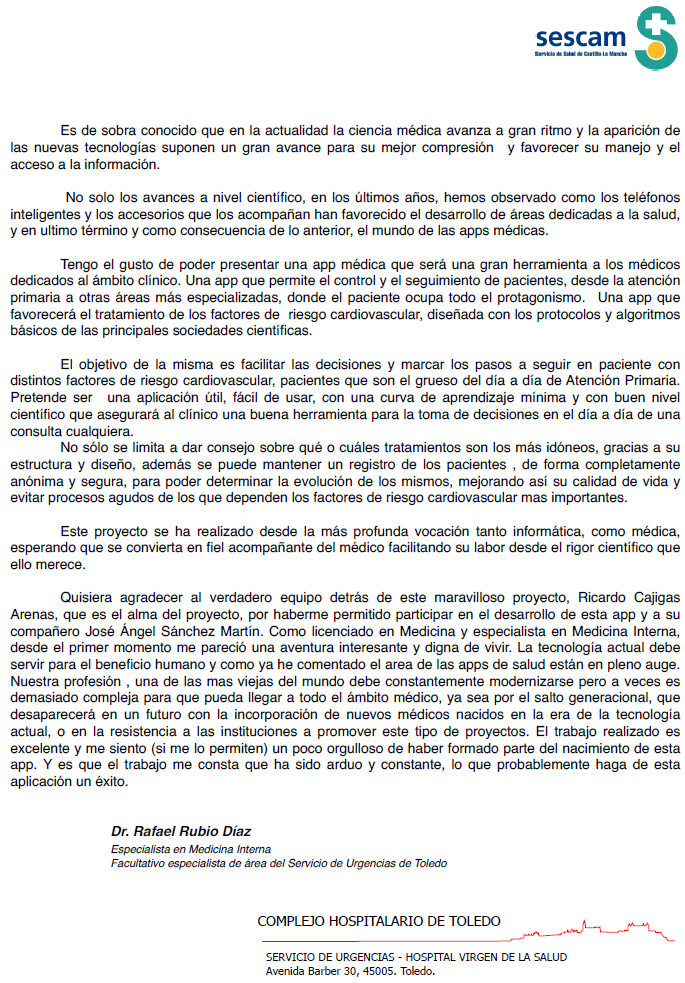
\includegraphics[width=0.90\textwidth]{prologo.png}    
   %\end{tabular}
\end{figure}

%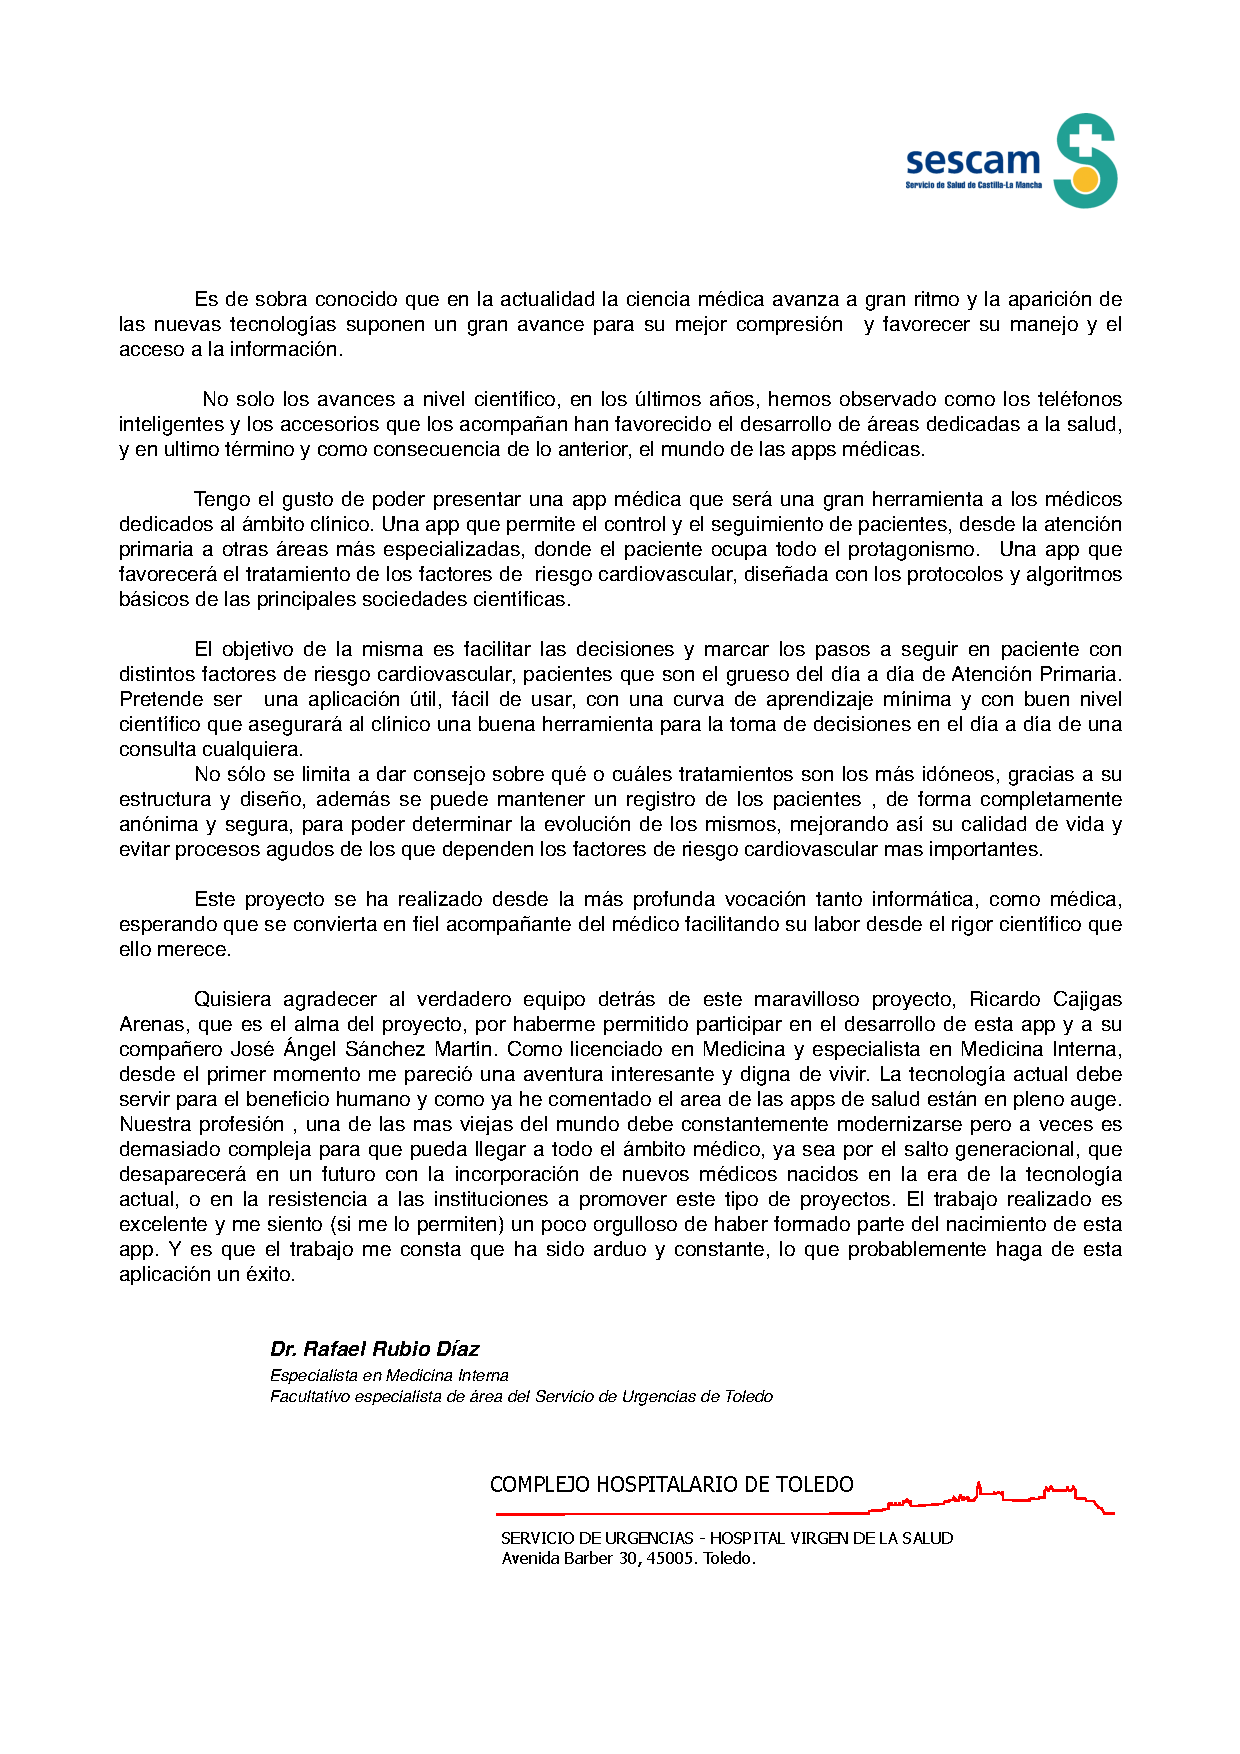
\includepdf{prologo}

%%%%%%%%%%%%%%%%%%%%%%%%%%%%%%%%%%%%%%%%%%%%%%%%%%%%%%%%%%%%%%%%%%%%%%%%%%%%%%%%%%%%%%%%%%%%%%%%%%%%%%%%%%%%%%%%%%%%%%%%%
%																			RESUMEN					                     															  %
%%%%%%%%%%%%%%%%%%%%%%%%%%%%%%%%%%%%%%%%%%%%%%%%%%%%%%%%%%%%%%%%%%%%%%%%%%%%%%%%%%%%%%%%%%%%%%%%%%%%%%%%%%%%%%%%%%%%%%%%%
\cleardoublepage
\begin{abstract}
%\setcounter{page}{1}
\addcontentsline{toc}{chapter}{Resumen}

El uso de aplicaciones en dispositivos móviles ha ido creciendo con el paso de los años, siendo hoy en día una herramienta fundamental en un amplio ámbito que va desde profesionales de las comunicaciones, economía, comercio y salud hasta las destinadas al ocio, viajes, deportes...

Este proyecto presenta una aplicación para Android que está enfocada al ámbito de la medicina y su objetivo específico es proporcionar una solución a uno de los problemas actuales que existe en el Hospital Virgen de la Salud de Toledo. Este dilema se refiere a la necesidad de agilizar el tratamiento de datos en los factores relativos al riesgo cardiovascular mediante el empleo de herramientas tecnológicas de última generación. Para lograr esta meta hemos diseñado una interfaz intuitiva y simple, proporcionando agilidad al médico en el cálculo del riesgo cardiovascular y asistencia complementaria a los métodos convencionales.

La aplicación está enfocada para ser gestionada por los médicos, permitiéndoles almacenar datos identificativos de un paciente y tratar la información concerniente a su estado en lo que respecta a la hipertensión arterial, el colesterol, la diabetes, el tabaquismo y el índice de masa corporal. Esta última característica será tomada como base por la app para la determinación del riesgo cardiovascular del paciente y la redacción de una breve sinopsis descriptiva que ayude al profesional sanitario en la prescripción de un tratamiento personalizado.
\end{abstract}

\begin{abstract}[english]
\addcontentsline{toc}{chapter}{Abstract}

The use of applications in mobile devices has been growing over the years, being nowadays a fundamental tool in a wide range, from professionals such us communications, economics, commerce and health to those destined to leisure, travel, sports ...

This project presents an Android application focused on the field of medicine, giving solution to one of the current problems that existed in the Hospital Virgen de la Salud of Toledo. This problem refers to the need to speed up the treatment of data on factors related to cardiovascular risk through the use of the last technological tools. To achieve this goal we have designed an intuitive and simple interface, providing agility to the doctor in calculating the cardiovascular risk, while being complemented by conventional methods.

The application is focused to be managed by doctors, allowing them to store patient's identification data and to manage information regarding their condition in relation to high blood pressure, cholesterol, diabetes, smoking and body mass index. This last characteristic will be taken by the app in order to determine the patient's cardiovascular risk and write a brief descriptive synopsis that helps the medical professional in the prescription of a personalized treatment.
\end{abstract}

\mainmatter


%%%%%%%%%%%%%%%%%%%%%%%%%%%%%%%%%%%%%%%%%%%%%%%%%%%%%%%%%%%%%%%%%%%%%%%%%%%%%%%%%%%%%%%%%%%%%%%%%%%%%%%%%%%%%%%%%%%%%%%%%
%																	INTRODUCCIÓN EN ESPAÑOL																				  %
%%%%%%%%%%%%%%%%%%%%%%%%%%%%%%%%%%%%%%%%%%%%%%%%%%%%%%%%%%%%%%%%%%%%%%%%%%%%%%%%%%%%%%%%%%%%%%%%%%%%%%%%%%%%%%%%%%%%%%%%%
\chapter{Introducci\'on}

La presencia cada vez más predominante de la digitalización trae como consecuencia una progresiva evolución hacia una sociedad donde una cantidad considerable de situaciones y problemas son resueltos mediante métodos informáticos y otros procedimientos automatizados. En otras palabras, nos acercamos a las circunstancias definidas bajo los términos de Internet of Things (IoT), SmartCities...

Teniendo esta idea en mente, organizamos una reunión con el Doctor Rafael Rubio Díaz y decidimos centrarnos en la diabetes como punto de partida. El propósito de esta iniciativa era conseguir la mejora del proceso de tratamiento de información en pacientes con diabetes. Explicado en más detalle, era el deseo del personal sanitario disponer de una herramienta que le posibilitase escribir informes médicos, consultar datos de un paciente y otras funciones fácilmente y sin necesidad de tener acceso a un ordenador de sobremesa, proporcionándoles así más movilidad y un comienzo en el abandono de los medios convencionales en favor de metodologías más modernas.

Tras un análisis del proyecto, se decidió expandir su alcance a los factores de riesgo cardiovasculares, obteniendo de esta forma una aplicación más completa y robusta. Esto supondría un mayor grado informativo de la condición del paciente, permitiendo así la creación de un tratamiento más preciso.

Se concibe este proyecto como Trabajo Fin de Grado correspondiente al Grado en Ingeniería Informática, con la firme idea de desarrollar una aplicación móvil capaz de ayudar en el marco de la sanidad, otorgando rapidez en el cálculo del riesgo cardiovascular de los pacientes.

%MOTIVACION
\section{Motivaci\'on}

Queríamos llevar a cabo un proyecto que no tuviese como objetivo solamente la satisfacción de fines académicos, sino que además fuera de utilidad para un colectivo de la sociedad. 

Decidimos centrarnos en la rama de la sanidad por varios factores influyentes:

\begin{enumerate}
	\item El interes personal que sentíamos por esta especialidad del saber.

	\item Su retraso en la incorporación de nuevas aplicaciones móviles con respecto a otros campos.

	\item La casi inexistencia de aplicaciones que tratasen esta necesidad en específico. Algunos ejemplos quedan documentados en \textquotedbl Estado del arte \textquotedbl{} expuesto en este capítulo.
	%\MakeUppercase{Enfermedades Cardiovasculares}
	%\item Esta app presenta al médico con la facultad de gestionar los datos médicos actuales del paciente y la delimitación de su riesgo cardiovascular, al mismo tiempo que le dota de una mayor libertad y prontitud acercando así a estas personas a las nuevas tecnologías.
\end{enumerate}

%OBJETIVOS
\section{Objetivos}

El objetivo principal del proyecto es el desarrollo de una herramienta, en concreto de una aplicación móvil, que asista en la determinación de la probabilidad del paciente de padecer enfermedades cardiovasculares, así como en el almacenamiento de la información pertinente y la especificación del tratamiento asignado.

El presente Trabajo Fin de Grado tiene los siguientes objetivos específicos:

\begin{itemize}
    \item Planificar un análisis de los aspectos dominantes que concluyen en el sufrimiento de dolencias del corazón o relacionadas con los vasos sanguíneos, con el fin de organizarlos e incluir aquellos que se consideren más adecuados y con mayor influencia en la evolución de estas enfermedades.

    \item Diseñar y concebir una aplicación móvil que resulte sencilla, atractiva e intuitiva, consiguiendo captar el interés de los usuarios ofreciéndoles una herramienta práctica para desempeñar su trabajo.
    
    \item Abstraer la información primordial de los datos introducidos acerca de un paciente por el médico, con el fin de determinar el índice REGICOR y delimitar los datos que servirán de punto de partida para el tratamiento.
    
    \item Plantear y elaborar una base de datos relacional para gestionar el almacenaje de toda la información generada por la app. 
    
    \item Establecer un sistema que permita a los médicos la colaboración entre ellos mediante la participación conjunta en la actualización de la condición de un único paciente.
    
    \item Garantizar la autenticidad de los registros realizados por el médico mediante la introducción de un rol de administrador, que tendrá privilegios para aceptar o rechazar los nuevos usuarios y modificar los datos personales de cualquier médico o paciente. 
\end{itemize}

%ESTADO DEL ARTE
\section{Estado del arte}

Con el fin de determinar el grado de impacto que pueda tener este proyecto, hemos realizado una investigación de posibles aplicaciones con objetivos o rasgos similares. Nuestro estudio ha revelado la existencia de varias aplicaciones con rasgos similares, o metas semejantes a las planeadas por nuestra aplicación. Citamos a continuación varios de los potenciales competidores:

\noindent
\textbf {Appteca }

\includegraphics[height=0.7cm]{hipertension_icon.jpg}

\includegraphics[height=0.7cm]{riesgo-cardiovascular_icon.jpg}  

\noindent
Es un  proyecto llevado a cabo por Sociedad Española de Cardiología y la Sociedad Española de Medicina, en las que incluyen varias aplicaciones relacionadas con el riesgo cardiovascular; Riesgo cardiovascular e Hipertensión arterial.

\noindent \url{http://appteca.es/}

\noindent
\textbf {PSCV}

\includegraphics[height=0.7cm]{PSCV_icon.jpg}

\noindent
Permite calcular una aproximación del riesgo cardiovascular con los fines y tratamientos asociados a cada nivel de riesgo. Ofrece información sobre el diagnóstico, manejo y seguimiento en la diabetes tipo 2, hipertensión arterial, infarto agudo al miocardio...

\noindent \url{https://play.google.com/store/apps/details?id=com.celmedia.minsal.pscv&hl=es_419} 

\noindent
\textbf {ASCVD Risk Estimator}
\ 
\includegraphics[height=0.7cm]{ASCVD_icon.jpg}

\noindent
Proporciona acceso rápido a recomendaciones específicas para los riesgos estimados por el calculador a la vez que vez que referencia información relacionado con terapia, monitorización y estilo de vida que puede interesar a pacientes y médicos.

\noindent \url{https://play.google.com/store/apps/details?id=org.acc.cvrisk&hl=es_419}

En definitiva, hay varias aplicaciones con una meta temática afín. No obstante, nuestra aplicación presenta funcionalidades únicas no cubiertas por las mencionadas anteriormente que le proporciona un carácter innovador. 
Algunas de estas novedades son sus funcionalidades centradas en la figura del médico en contraposición con el enfoque habitual en el paciente, la facilitación de métodos para la búsqueda de perfiles (pacientes y médicos) y la colaboración conjunta entre médicos para el tratamiento del paciente.

%ESTRUCTURA DE LA MEMORIA
\section{Estructura de la mem\'oria}

La memoria está organizada en cinco capítulos siendo el primero de estos la presente introducción.

En el capítulo 2 se hace una explicación detallada de las funcionalidades de la aplicación móvil. Este punto incluye los respectivos diagramas de actividades y las ventana correspondientes a cada uno de ellos.

El capítulo 3 especifica los distintos módulos que constituyen el sistema. 

En el capítulo 4 se profundiza en la estructura y la disposición decidida para el diseño de la base de datos relacional en la que se almacena la información.

El capítulo 5 puntualiza las tecnologías de las que se ha valido la aplicación, exponiendo las características de cada una de ellas y la línea de pensamiento que nos ha llevado a escogerlas para el desarrollo de este proyecto.

En el capítulo 6 se exponen las principales conclusiones de este proyecto. Se tratan aspectos como la experiencia de los desarrolladores de este trabajo y las nuevas competencias adquiridas durante el mismo.

El capítulo 7 presenta un plan de mejora futuro. Con las ideas planteadas se pretende incrementar las funcionalides ofrecidas por nuestra aplicación y acrecentar su competitividad en el mercado.

El capítulo 8 delimita el alcance de la contribución de cada uno de los miembros del grupo.


%%%%%%%%%%%%%%%%%%%%%%%%%%%%%%%%%%%%%%%%%%%%%%%%%%%%%%%%%%%%%%%%%%%%%%%%%%%%%%%%%%%%%%%%%%%%%%%%%%%%%%%%%%%%%%%%%%%%%%%%%
%																	INTRODUCCIÓN EN INGLÉS																				  %
%%%%%%%%%%%%%%%%%%%%%%%%%%%%%%%%%%%%%%%%%%%%%%%%%%%%%%%%%%%%%%%%%%%%%%%%%%%%%%%%%%%%%%%%%%%%%%%%%%%%%%%%%%%%%%%%%%%%%%%%%
\addtocounter{chapter}{-1}
\selectlanguage{english}
\chapter{Introduction}
\phantomsection

The increasingly predominant presence of digitalization results in a progressive evolution towards a society where a considerable number of situations and problems are solved through computer methods and other automated procedures. In other words, we approach the circumstances defined under the terms of Internet of Things (IoT), SmartCities...

Having this idea in mind, we organized a meeting with the Doctor Rafael Rubio Diaz and decided to focus on diabetes as the starting point. The purpose of this initiative was to improve the process of information processing in patients with diabetes. Explained in more detail, it was the medical staff$'$s desire to have a tool that would enable them to write medical reports, consult a patient$'$s data and other functions easily and without requiring access to a desktop computer, thus giving them more mobility and a beginning in the abandonment of conventional means on favour of more modern methodologies.

After an analysis of the project, it was decided to expand its reach to cardiovascular risk factors, obtaining a more complete and robust application. This would imply a greater informative degree of the patient$'$s condition, thus allowing the creation of a more precise treatment.

This project was conceived as an End of Grade Work corresponding to the Degree in Computer Engineering, with the firm idea of developing a mobile application capable of helping within the framework of health, granting speed in the calculation of cardiovascular risk of patients.

%MOTIVATION
\section{Motivation}

We wanted to carry out a project that was not only aimed at satisfying academic goals, but was also useful for a group of society.

We decided to focus on the health sector because of several influential factors:

\begin{enumerate}
	\item The personal interest we felt in this specialty of knowledge.

	\item Its delay in incorporating new mobile applications with respect to other fields.

	\item The almost nonexistence of applications that addressed this need in specific. Some examples are documented in \textquotedbl State of the art \textquotedbl {} discussed in this chapter.
	%\MakeUppercase{Enfermedades Cardiovasculares}
	%\item This app presents the doctor with the power to manage the patient's current medical data and the delimitation of his cardiovascular risk, while giving him greater freedom and promptness thus bringing these people to the new technologies.
\end{enumerate}

%OBJECTIVES
\section{Objectives}

The main objective of the project is the development of a tool, specifically a mobile application, that assists in determining the patient's likelihood of suffering cardiovascular diseases, as well as the storage of the relevant information and the specification of the assigned treatment.

The present End of Degree Work has the following specific objectives:

\begin{itemize}
    \item Plan an analysis of the dominant aspects that end in the suffering of heart ailments or related to the blood vessels, in order to organize them and to include those that are considered more suitable and with greater influence in the evolution of these diseases.

    \item Designing and designing a mobile application that is simple, attractive and intuitive, capturing users' interest by offering them a practical tool to carry out their work.
    
    \item Abstracting the primary information about the data entered about a patient by the doctor, in order to determine the REGICOR index and delimit the data that will serve as a starting point for treatment.
    
    \item Arrange and build a relational database to manage the storage of all the information generated by the app. 
    
    \item Establish a system that allows physicians to collaborate with each other through joint participation in updating the condition of a single patient.
    
    \item Guarantee the authenticity of the records made by the doctor by introducing an administrator role, which will have privileges to accept or reject new users and modify the personal data of any doctor or patient. 
\end{itemize}

%STATE OF THE ART
\section{State of the art}

In order to determine the degree of impact that this project may have, we have carried out an investigation of possible applications with similar objectives or traits. Our study has revealed the existence of several applications with similar traits, or goals similar to those planned by our application. We cite below several of the potential competitors:

\noindent
\textbf {Appteca }

\includegraphics[height=0.7cm]{hipertension_icon.jpg}

\includegraphics[height=0.7cm]{riesgo-cardiovascular_icon.jpg}  

\noindent
It is a project carried out by the Spanish Society of Cardiology and the Spanish Society of Medicine, which include several applications related to cardiovascular risk; Cardiovascular risk and Hypertension.

\noindent \url{http://appteca.es/}

\noindent
\textbf {PSCV}

\includegraphics[height=0.7cm]{PSCV_icon.jpg}

\noindent
It allows to calculate an approximation of the cardiovascular risk with the purposes and treatments associated to each level of risk. It offers information on the diagnosis, management and follow-up in type 2 diabetes, hypertension, myocardial infarction ...

\noindent \url{https://play.google.com/store/apps/details?id=com.celmedia.minsal.pscv&hl=es_419} 

\newpage
\noindent
\textbf {ASCVD Risk Estimator}

\includegraphics[height=0.7cm]{ASCVD_icon.jpg}

\noindent
It provides quick access to specific recommendations for the calculator's estimated risks, while referring to information related to therapy, monitoring and lifestyle that may be of interest to patients and physicians.

\noindent \url{https://play.google.com/store/apps/details?id=org.acc.cvrisk&hl=es_419}

In short, there are several applications with a related thematic goal. However, our application presents unique functionalities not covered by the aforementioned that provides an innovative character. 
Some of these innovations are its functionalities focused on the figure of the doctor as opposed to the usual approach in the patient, the facilitation of methods for the search of profiles (patients and doctors) and the joint collaboration between doctors for the treatment of the patient.

%MEMORY STRUCTURE
\section{Memory structure}

The memory is organized into five chapters, the first of which is the present introduction.

Chapter 2 provides a detailed explanation of the features of the mobile application. This point includes the respective activity diagrams and the corresponding window of each one.

Chapter 3 specifies the different modules that make up the system.

Chapter 4 explores the structure and willingness to design the relational database in which information is stored.

Chapter 5 points out the technologies that the application has validated, exposing the characteristic of each one of them and the line of thought that has led us to choose them for the development of this project.

Chapter 6 sets out the main conclusions of this project. It deals with aspects such as the experience of the developers of this work and the new skills acquired during it.

Chapter 7 presents a plan for future improvement. With the ideas put forward we intend to increase the functionalities offered by our application and increase its competitiveness in the market.

Chapter 8 delimits the scope of the contribution of each member of the group.


%%%%%%%%%%%%%%%%%%%%%%%%%%%%%%%%%%%%%%%%%%%%%%%%%%%%%%%%%%%%%%%%%%%%%%%%%%%%%%%%%%%%%%%%%%%%%%%%%%%%%%%%%%%%%%%%%%%%%%%%%
%																	ESPECIFICACIÓN DE LA APLICACION																			  %
%%%%%%%%%%%%%%%%%%%%%%%%%%%%%%%%%%%%%%%%%%%%%%%%%%%%%%%%%%%%%%%%%%%%%%%%%%%%%%%%%%%%%%%%%%%%%%%%%%%%%%%%%%%%%%%%%%%%%%%%%
\selectlanguage{spanish}
\chapter{Especificación de la aplicaci\'on}

En esta sección vamos a introducir las funciones desempeñadas por nuestra aplicación. Los cometidos primordiales de la misma son dar de alta a los pacientes, calcular su índice de riesgo cardiovascular y ofrecer una orientación para establecer el tratamiento.

Asimismo, la aplicación presenta un amplio rango de funcionalidades que describiremos en detalle en los puntos posteriores. En primer lugar, expondremos las funcionalidades de los médicos. En segundo lugar, explicamos las competencias reservadas al administrador. 
Por último, concluimos introduciendo las facultades comunes a ambos perfiles.

%%%%%%%%%%%MEDICO
\section {Compentencias disponibles para el médico}
Una responsabilidad característica del profesional sanitario es la aportación datos para el alta del paciente. Este rol requiere de un método (Mi perfil) que le conceda la capacidad de manipular sus datos personales.
Con el fin de asistir al médico en el diagnostico del tratamiento se facilita el acceso a una BDDD de fármacos. Si desea constatar que los resultados obtenidos reponden a una imagen verídica, o simplemente analizar la exactitud de las fórmulas empleadas, se introduce la pestaña de algorítmos.

Las interacciones que puede llevar a cabo exclusivamente el personal médico se ilustra en la Figura2.1.

\newpage
\begin{landscape}
	\begin{figure}[H]
	\centering
	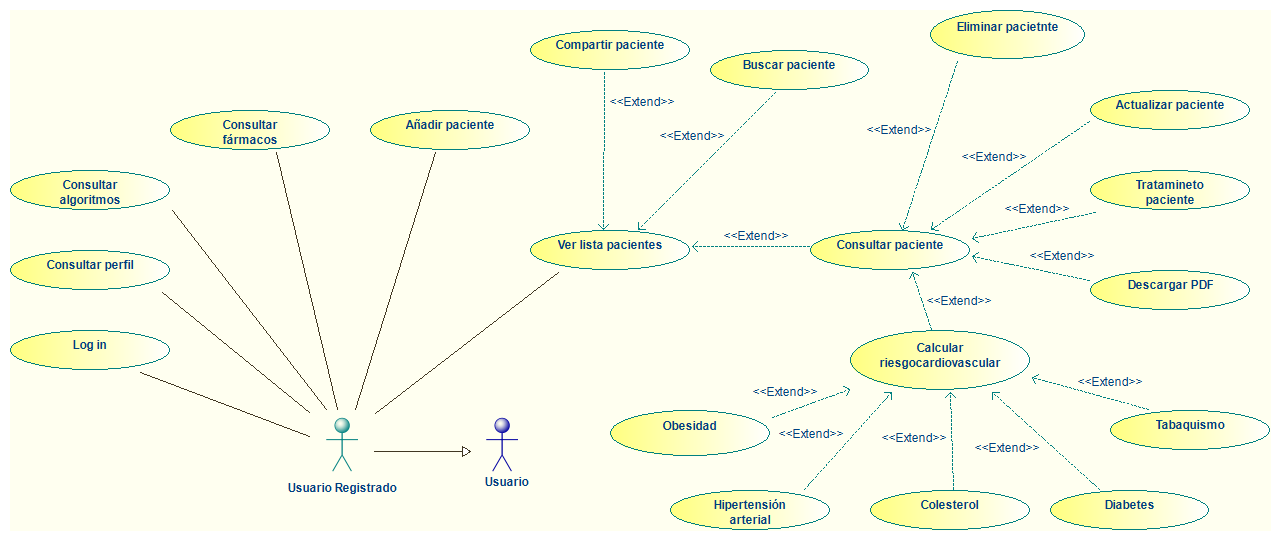
\includegraphics[height= 10cm]{diagramas/UsuarioRegistradoUseCasediagram.png}
	\caption{Diagrama de caso de uso - Usuario Registrado}
	\end{figure}
\end{landscape}


\vfill
%MI PERFIL
\subsection {Mi perfil}

Es imprescindible que el usuario tenga poder administrativo sobre sus propios datos (Figura 2.2). La causa es que es habitual que el individuo necesite modificar alguno de ellos; ya sea por haber errado en la introducción de la información durante el registro, por modificar su correo electrónico o por querer actualizar su contraseña. (Figura 2.3)

\begin{figure}[H]
\centering
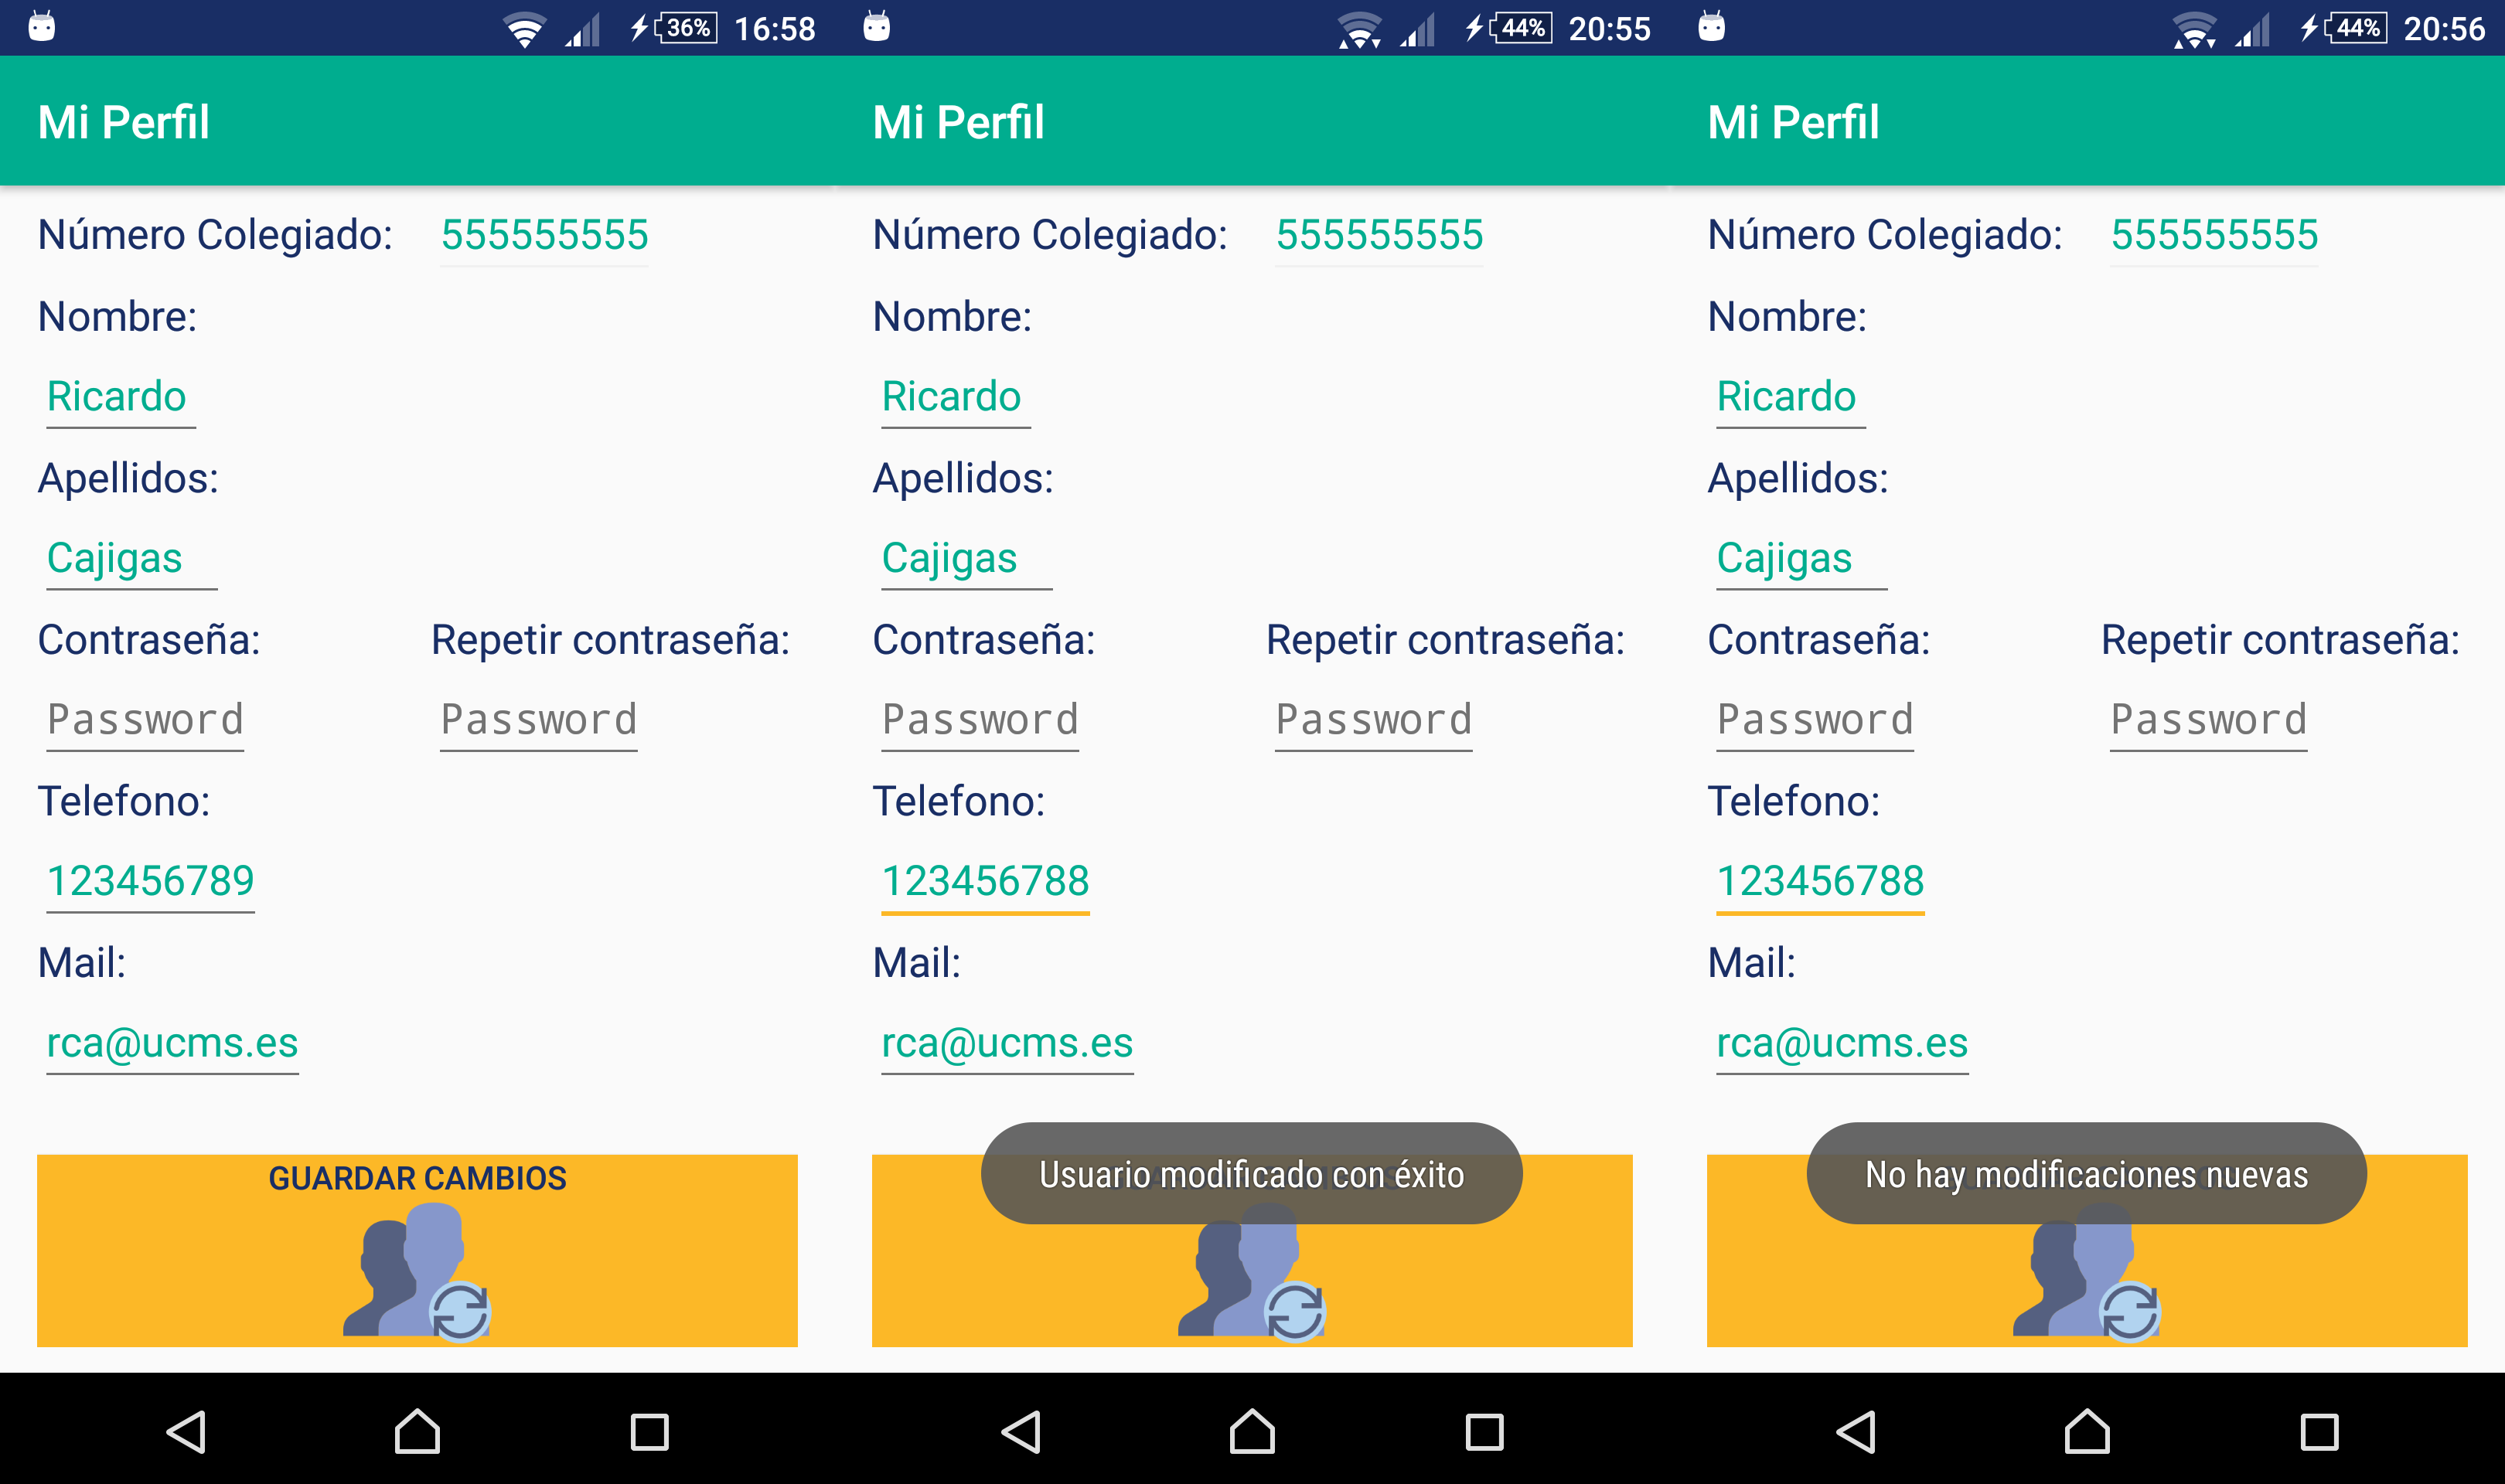
\includegraphics[height= 7cm]{capturas/mi_perfilFull.png}
\caption{Ventana - Mi Perfil}
\end{figure}

\vfill
\begin{figure}[H]
\centering
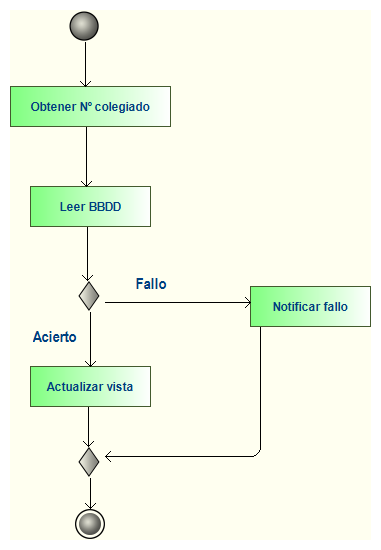
\includegraphics[height= 11cm]{diagramas/VerperfilActivitydiagram.png}
\caption{Diagrama de actividad -  Mi Perfil}
\end{figure}

\vfill
%NUEVO PACIENTE
\subsection {Nuevo paciente}

Inscribe los datos de un nuevo paciente bajo el médico logueado. Para ello se le identificará mediante un ID que responderá a la siguiente formula; las iniciales del nombre y apellidos seguido de su fecha de nacimiento en formato ddmmyy (Figura 2.4). También se facilitará la información relativa al género. (Figura 2.5)

*En aquellos casos en los que el paciente no disponga de dos apellidos, se repetirá la inicial del primer apellido dos veces. Es importante mencionar que este sistema no contempla aquellos individuos que excedan los dos dígitos de edad.

\begin{figure}[H]
\centering
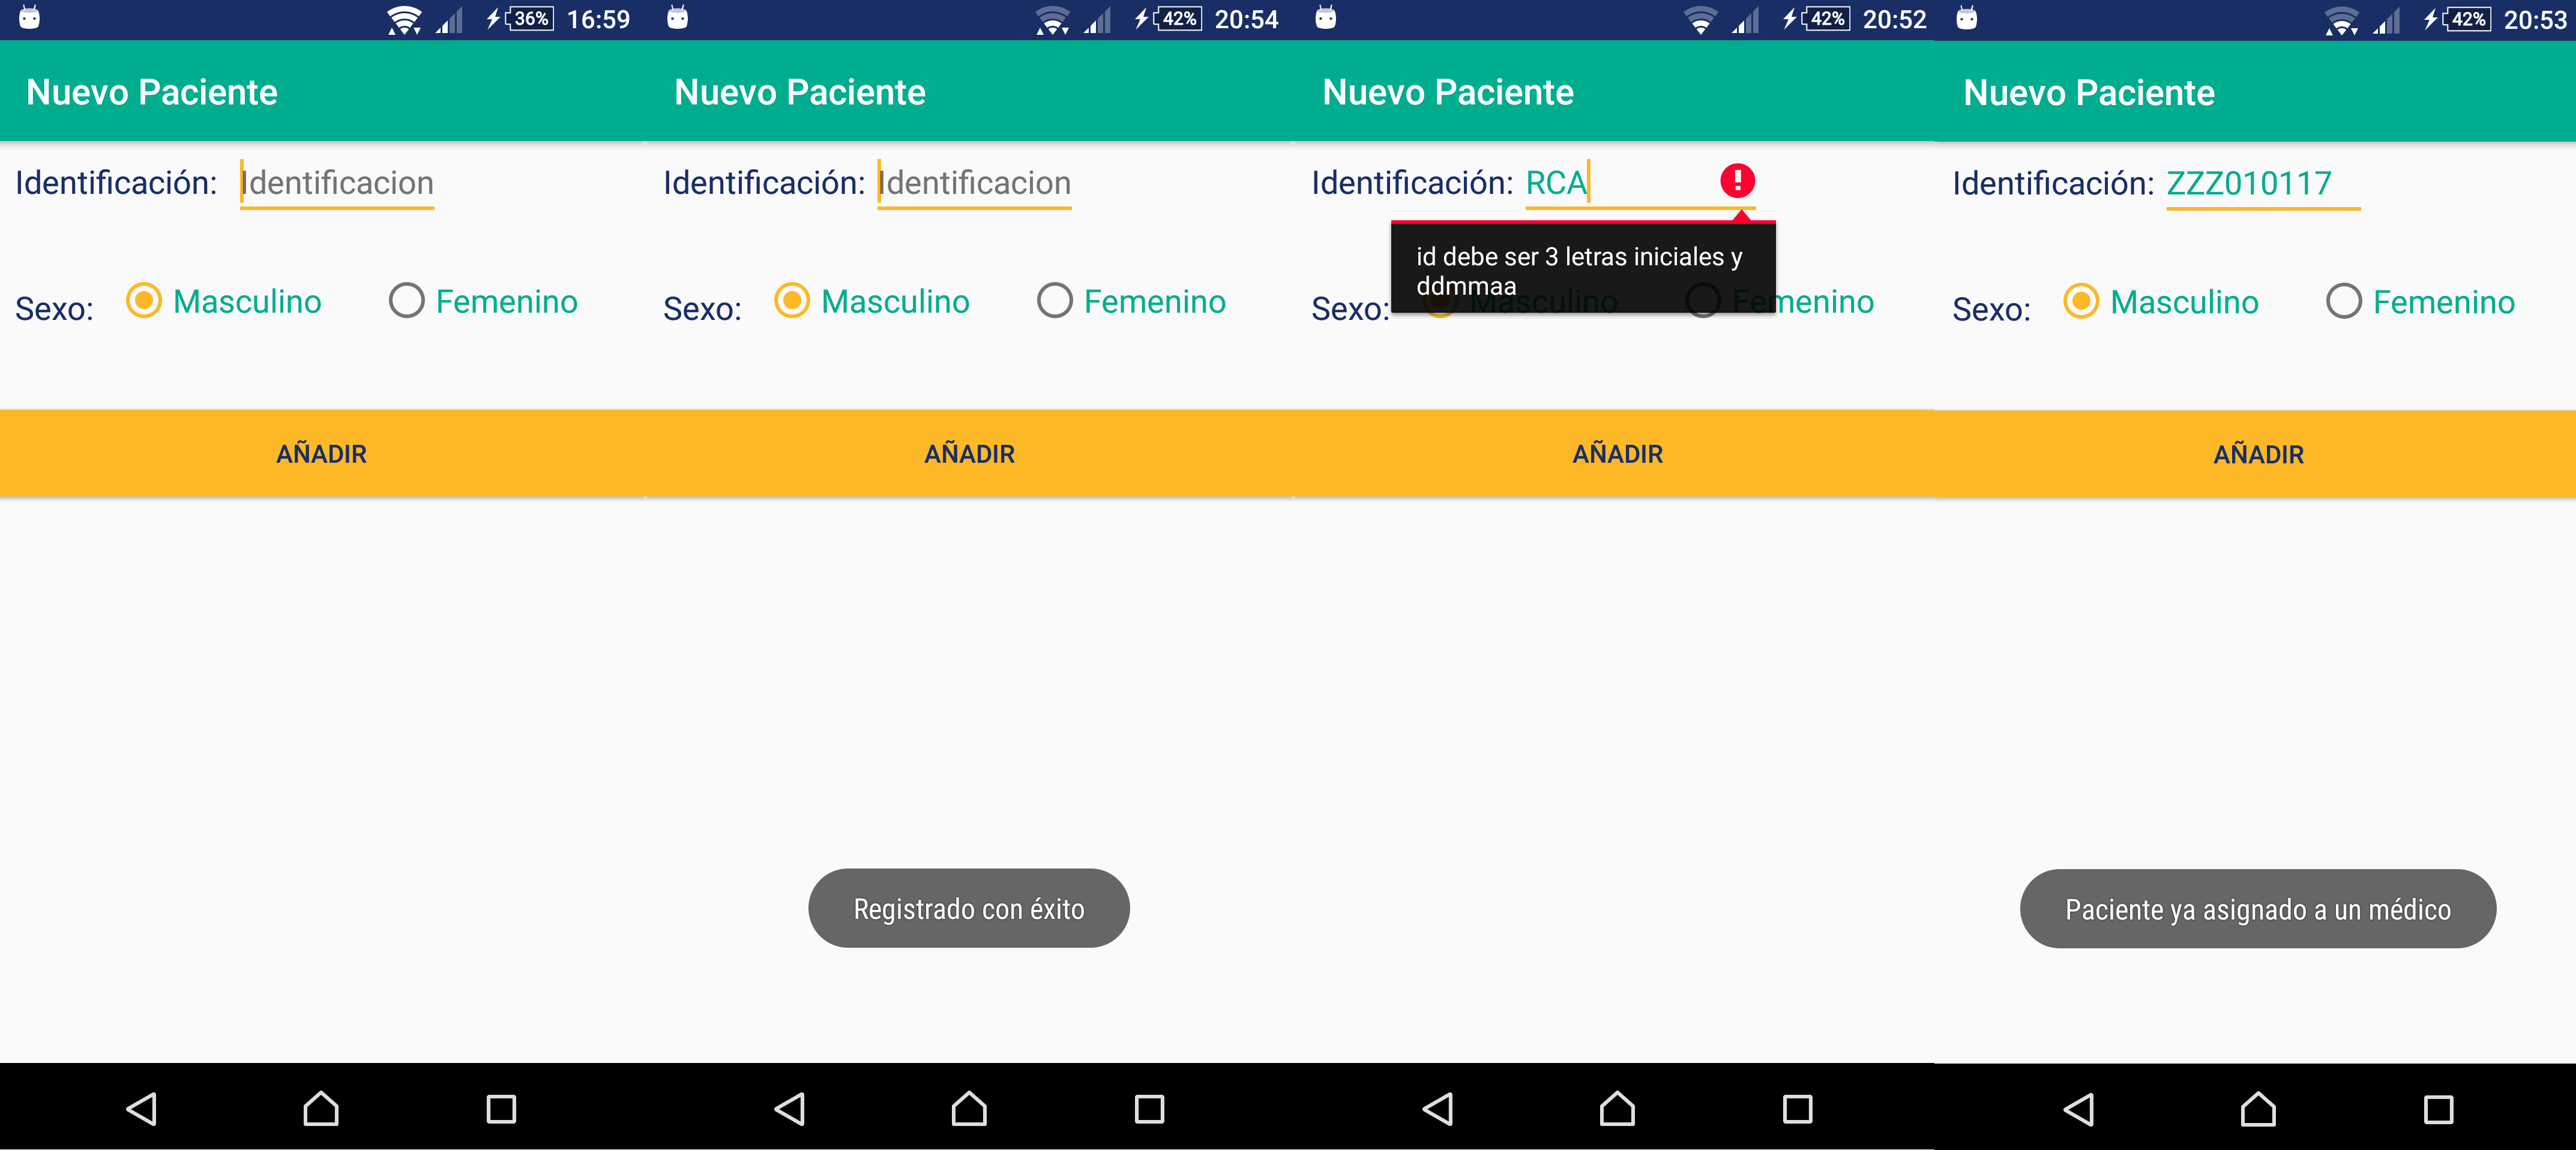
\includegraphics[height= 6.7cm]{capturas/nuevoPacienteFull.png}
\caption{Ventana - Nuevo Paciente}
\end{figure}

\begin{figure}[H]
\centering
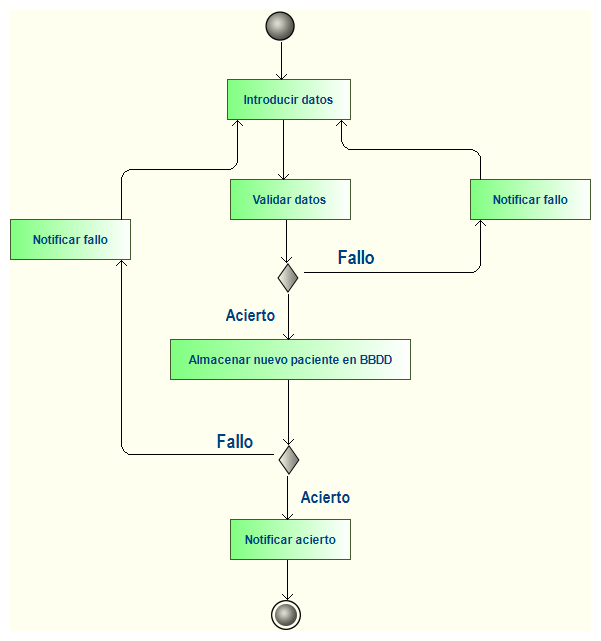
\includegraphics[height= 11cm]{diagramas/AnadirpacienteActivitydiagram.png}
\caption{Diagrama de actividad - Nuevo Paciente}
\end{figure}

%CONSULTAR ALGORITMOS
\subsection {Consultar algorítmos}

Permite informarse sobre nuestras formulas automatizadas de las que hacemos uso para calcular los resultados de los factores de influencia en el cálculo del riesgo cardiovascular: diabetes, colesterol, hipertensión arterial, índice de masa corporal, tabaquismo (Figura 2.6). Los algoritmos se presentan gráficamente en diagramas de flujo. (Figura 2.7)

\begin{figure}[H]
\centering
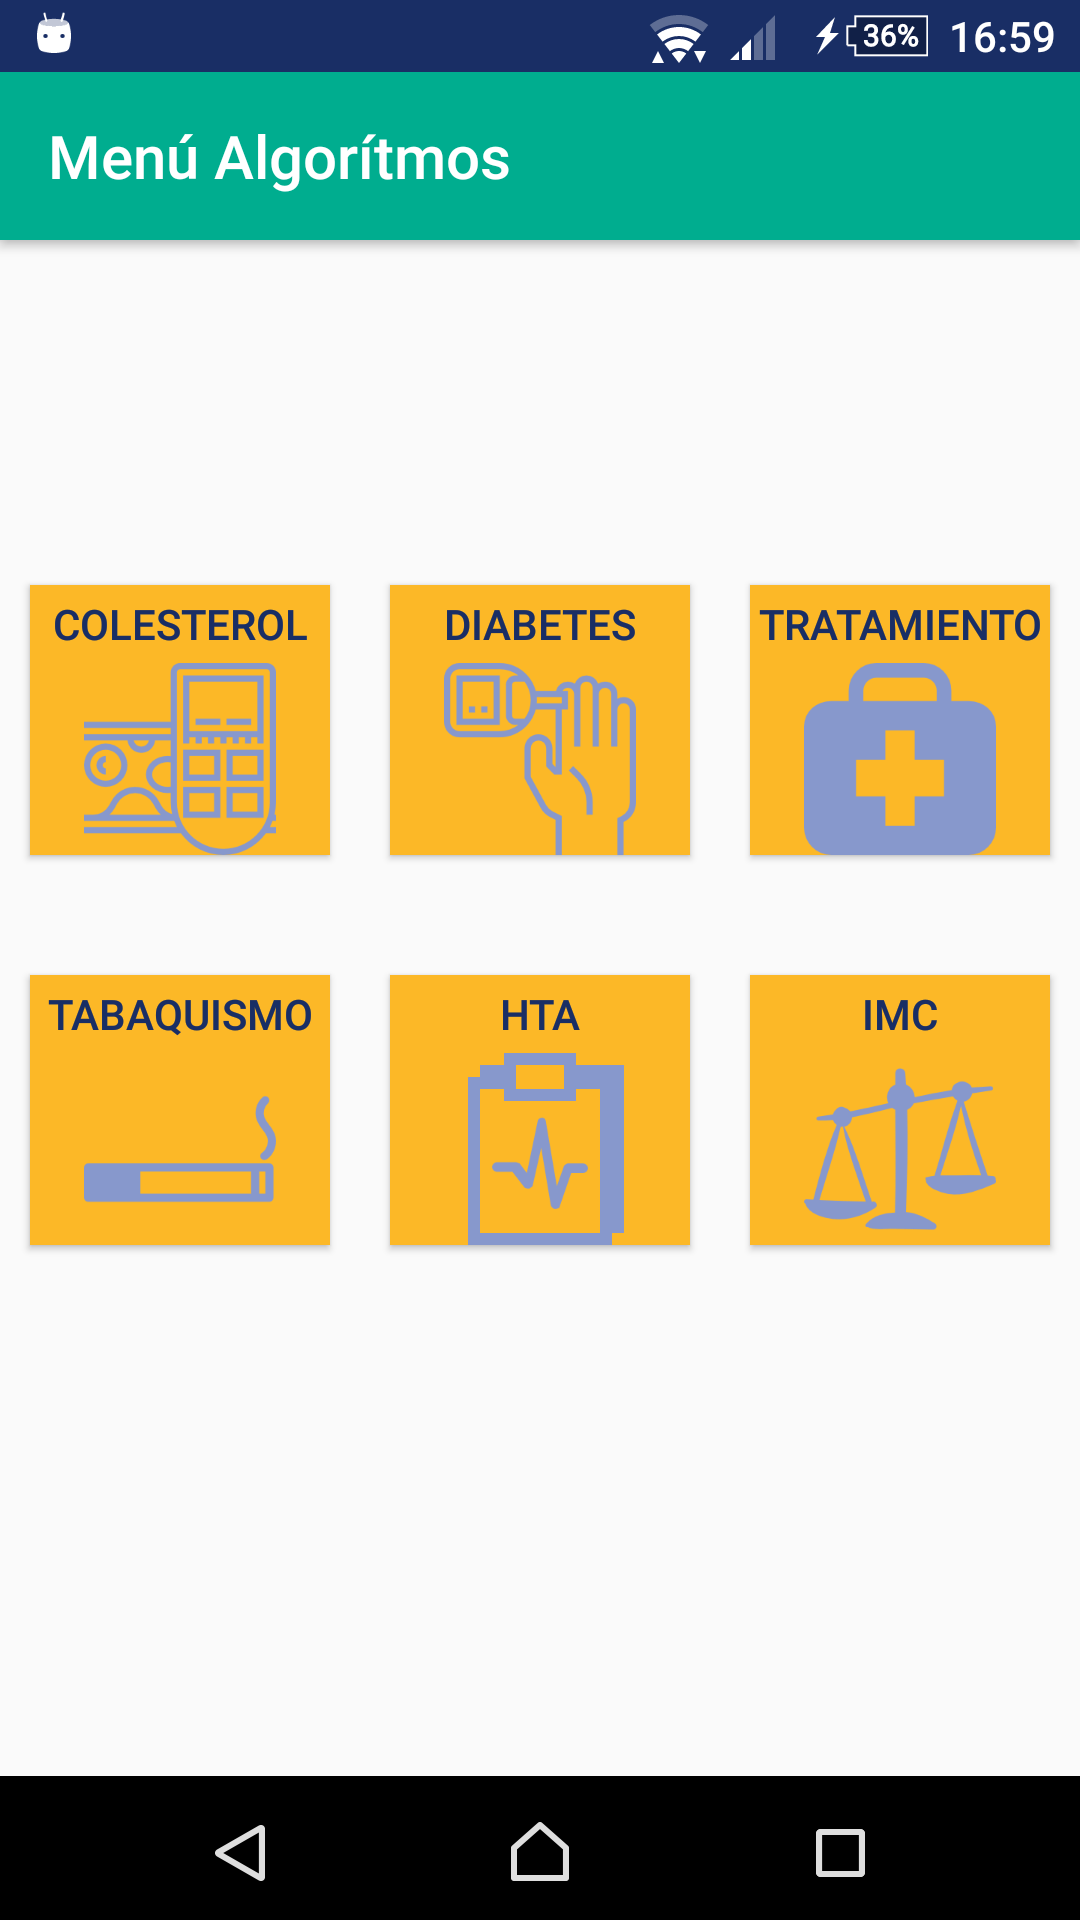
\includegraphics[height= 7cm]{capturas/algoritmos.png}
\caption{Ventana - Consultar Algorítmos}
\end{figure}

\begin{figure}[H]
\centering
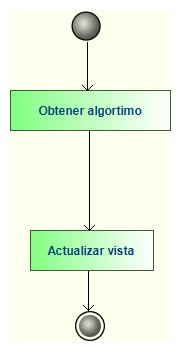
\includegraphics[height= 7cm]{diagramas/ConsultaralgoritmoActivitydiagram.png}
\caption{Diagrama de actividad -  Consultar Algorítmos}
\end{figure}

\vfill
%CONSULTAR FARMACOS
\subsection {Consultar fármacos}

El profesional accede a una base de datos exterior a la aplicación (\url {http://www.vademecum.es/medicamentos-a_1}) en la que se pueden consultar todos los medicamentos a considerar (Figura 2.8). Esta es ampliamente utilizada entre el personal sanitario, por lo que podemos confiar que se mantendrá actualizada con frecuencia. (Figura 2.9)

En un principio la idea original era crear nuestra propia base de datos de fármacos, un motor de búsqueda asociado y otras funcionalidades relativas a esta categoría. Sin embargo, tras estudiarlo concluimos que la carga en la aplicación no era algo que nos pudiéramos permitir en una aplicación de esta naturaleza. Todo esto nos llevó a modificar nuestros planes originales y ofrecer el servicio por medio de esta herramienta auxiliar.

\begin{figure}[H]
\centering
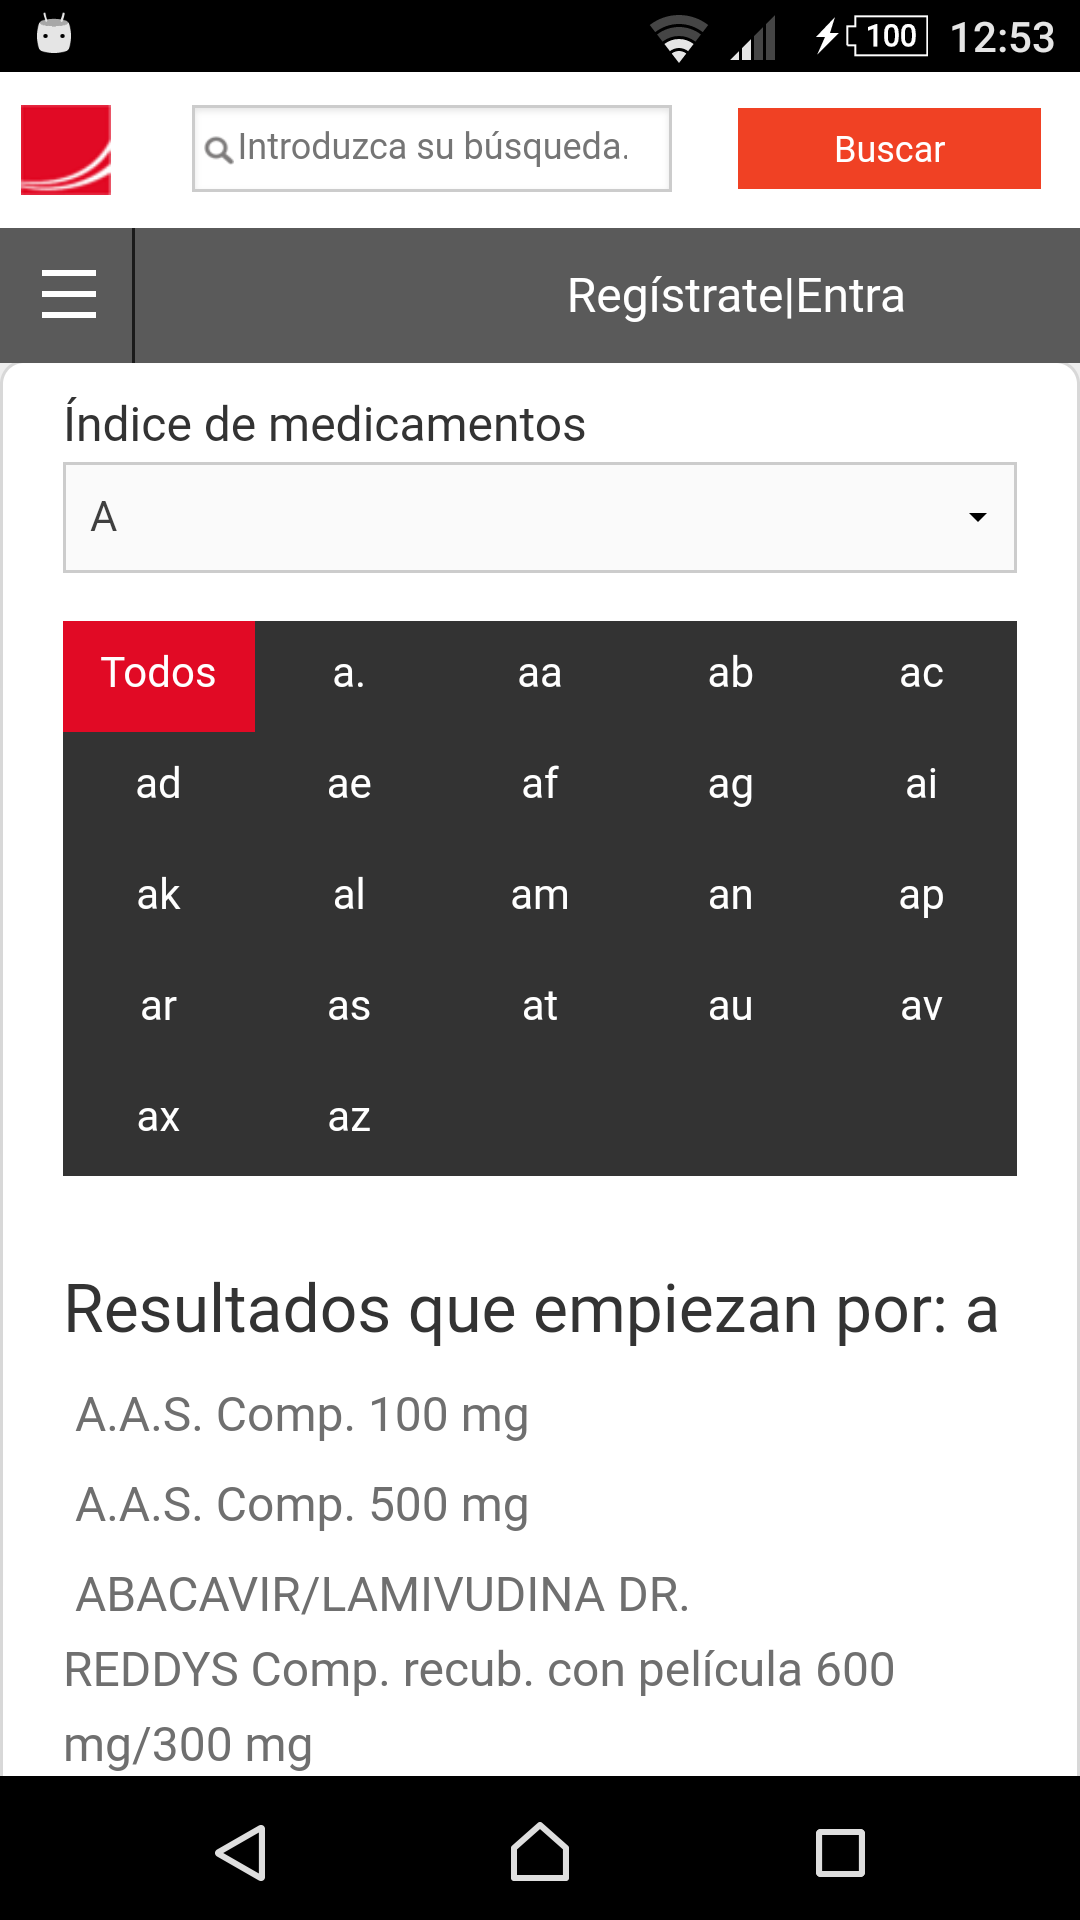
\includegraphics[height= 7cm]{capturas/farmacos.png}
\caption{Ventana - Consultar Fármacos}
\end{figure}

\begin{figure}[H]
\centering
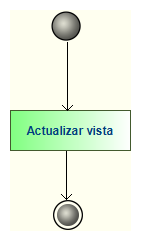
\includegraphics[height= 6cm]{diagramas/ConsultarfarmacosActivitydiagram.png}
\caption{Diagrama de actividad -  Consultar Fármacos}
\end{figure}

\vfill
%%%%%%%%%%%%ADMINISTRADOR
\section {Potestades asignadas al administrador}
La necesidad de gestionar el perfil anterior es esencial incluir un rol administrativo. Este supervisor decidirá la autenticidad de la información suministrada en los registros (Validar/Rechazar aspirante), asi como enmendar posibles errores al proveer o modificar las credenciales y atribuciones de los pacientes.

A continuación estas aptitudes quedan reflejadas en un diagrama. (Figura 2.10)

\begin{landscape}
	\begin{figure}[H]
	\centering
	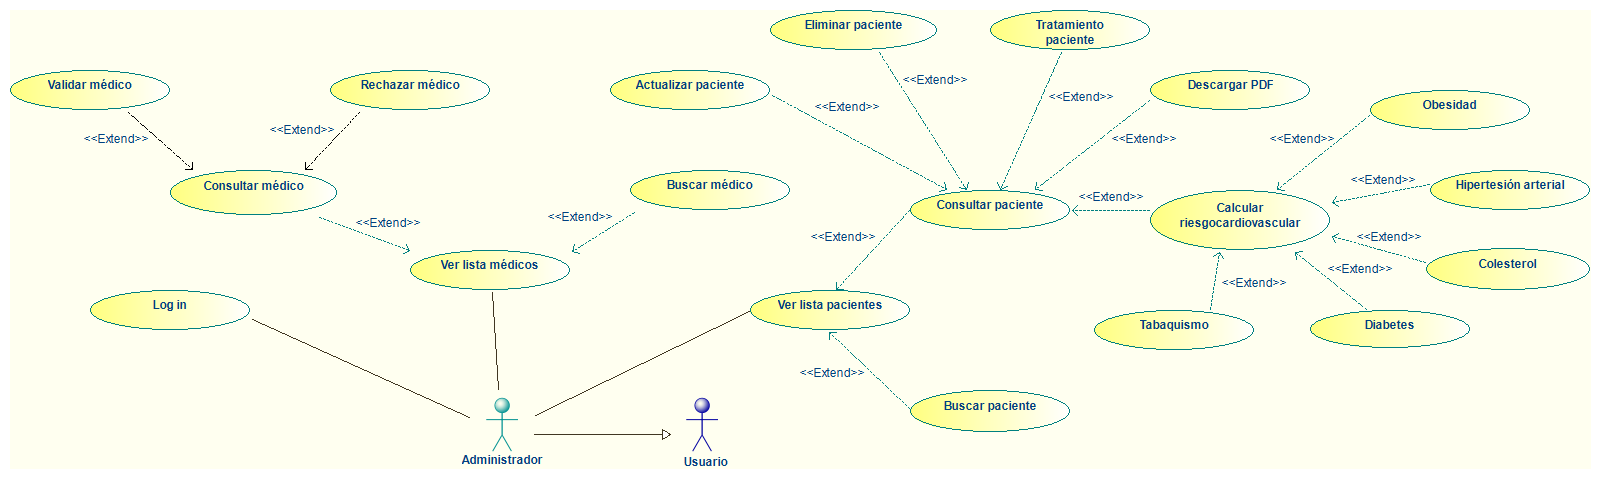
\includegraphics[height= 7cm]{diagramas/AdministradorUseCasediagram.png}
	\caption{Diagrama de caso de uso - Administrador}
	\end{figure}
\end{landscape}

\vfill
%LISTA ASPIRANTES
\subsection {Lista de aspirantes}

Como consecuencia de la necesidad de verificar si el usuario potencial realmente posee una identidad como profesional sanitario, se concretó esta funcionalidad con el fin de atender a este dilema. Se introduce el rol de administrador, el cual tiene capacidad para conceder acceso a la aplicación o rechazar al solicitante en función de los datos. Los aspirantes se muestran en este catálogo que identifica a cada elemento con su número de colegiado, nombre y apellidos (Figura 2.11). (Figura 2.12)

\begin{figure}[H]
\centering
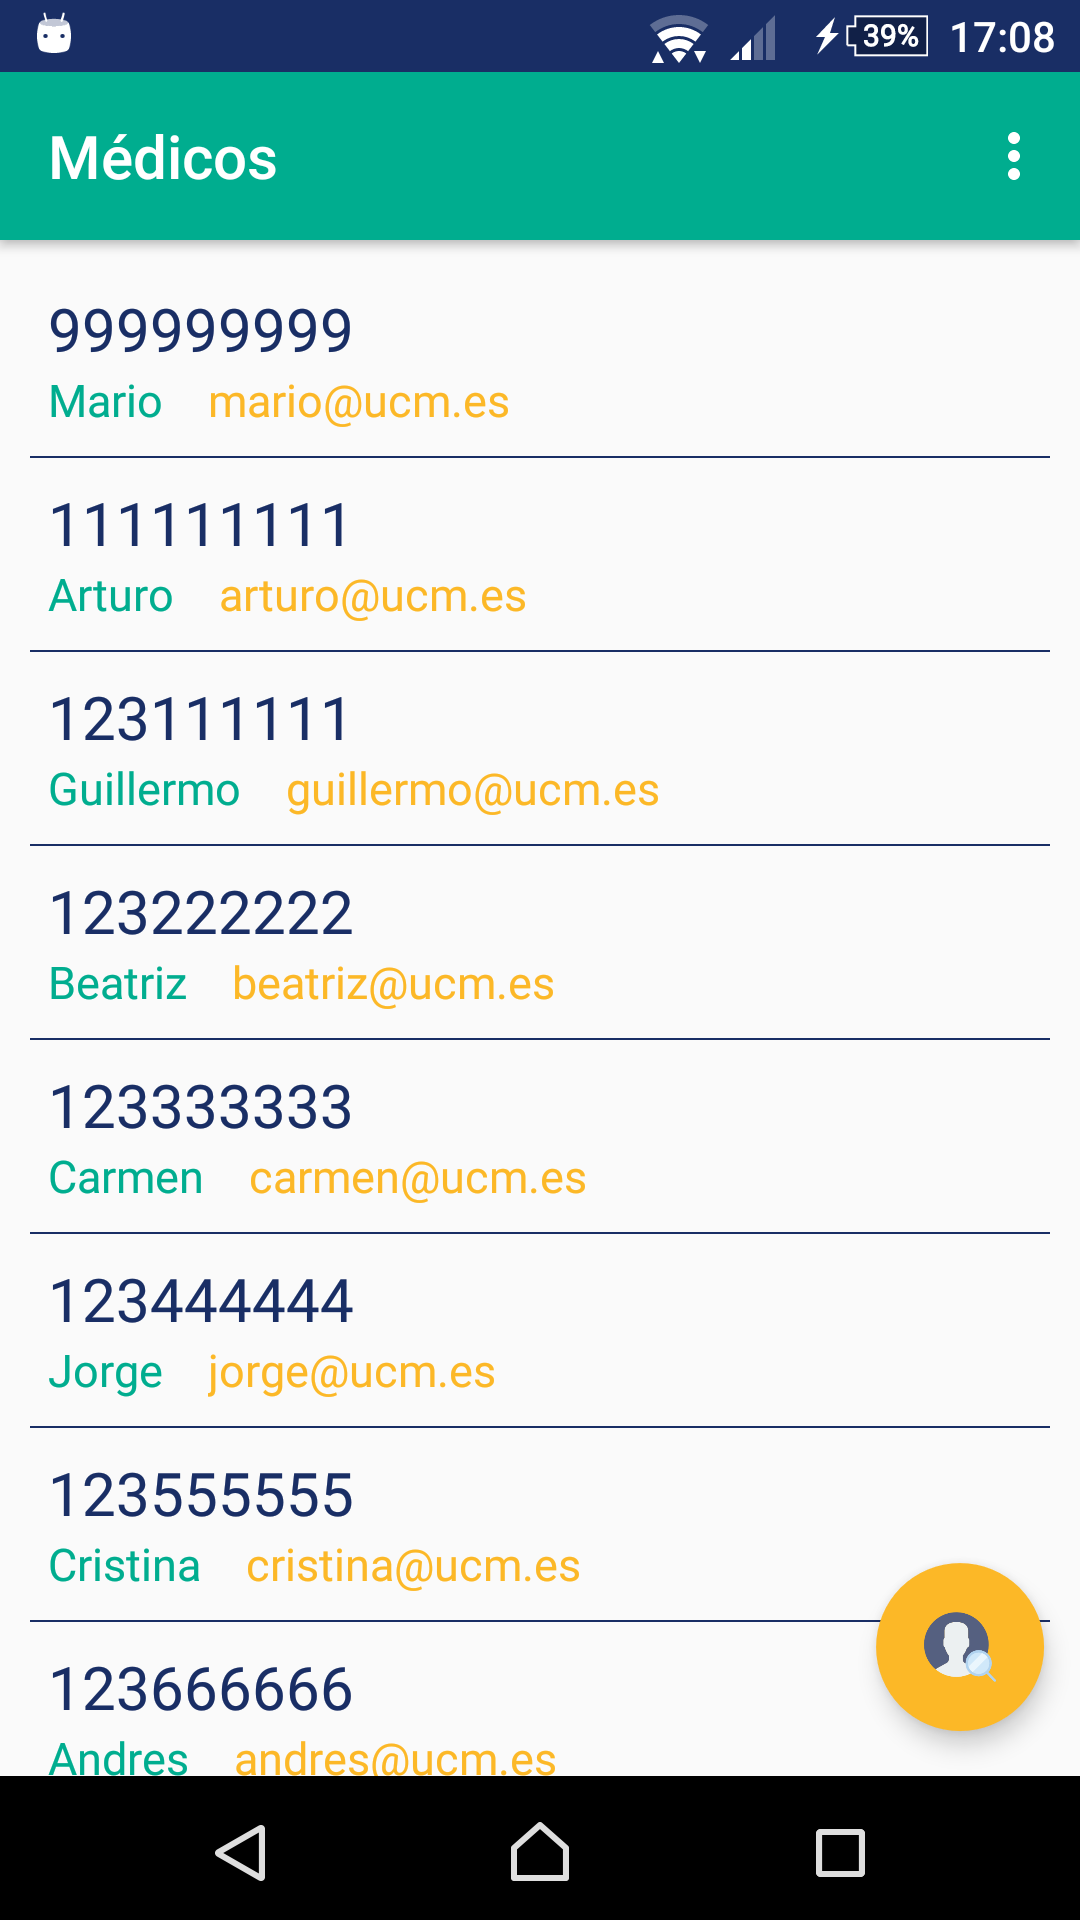
\includegraphics[height= 7cm]{capturas/medicos_lista.png}
\caption{Ventana -  Lista Aspirantes}
\end{figure}

\begin{figure}[H]
\centering
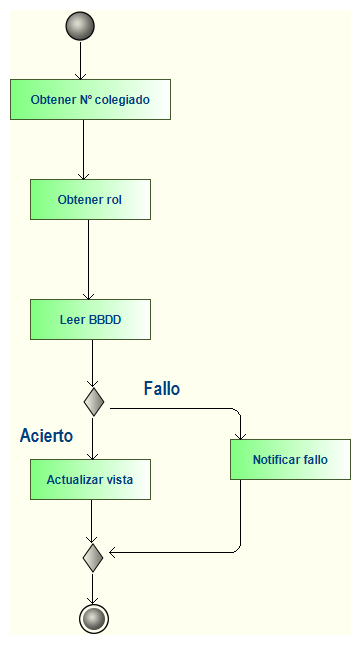
\includegraphics[height= 11cm]{diagramas/ListamedicosActivitydiagram.png}
\caption{Diagrama de actividad -  Lista Aspirantes}
\end{figure}

\vfill
%BUSCAR ASPIRANTES
\subsection {Buscar aspirante}

En numerosas ocasiones, el supervisor de la aplicación podría requerir localizar a un sujeto en específico. Como solución a este problema se introduce un motor de búsqueda, el cual ofrece filtrar por nombre, número de colegiado, mail y/o una combinación de estos últimos (Figura 2.13). (Figura 2.14)

\begin{figure}[H]
\centering
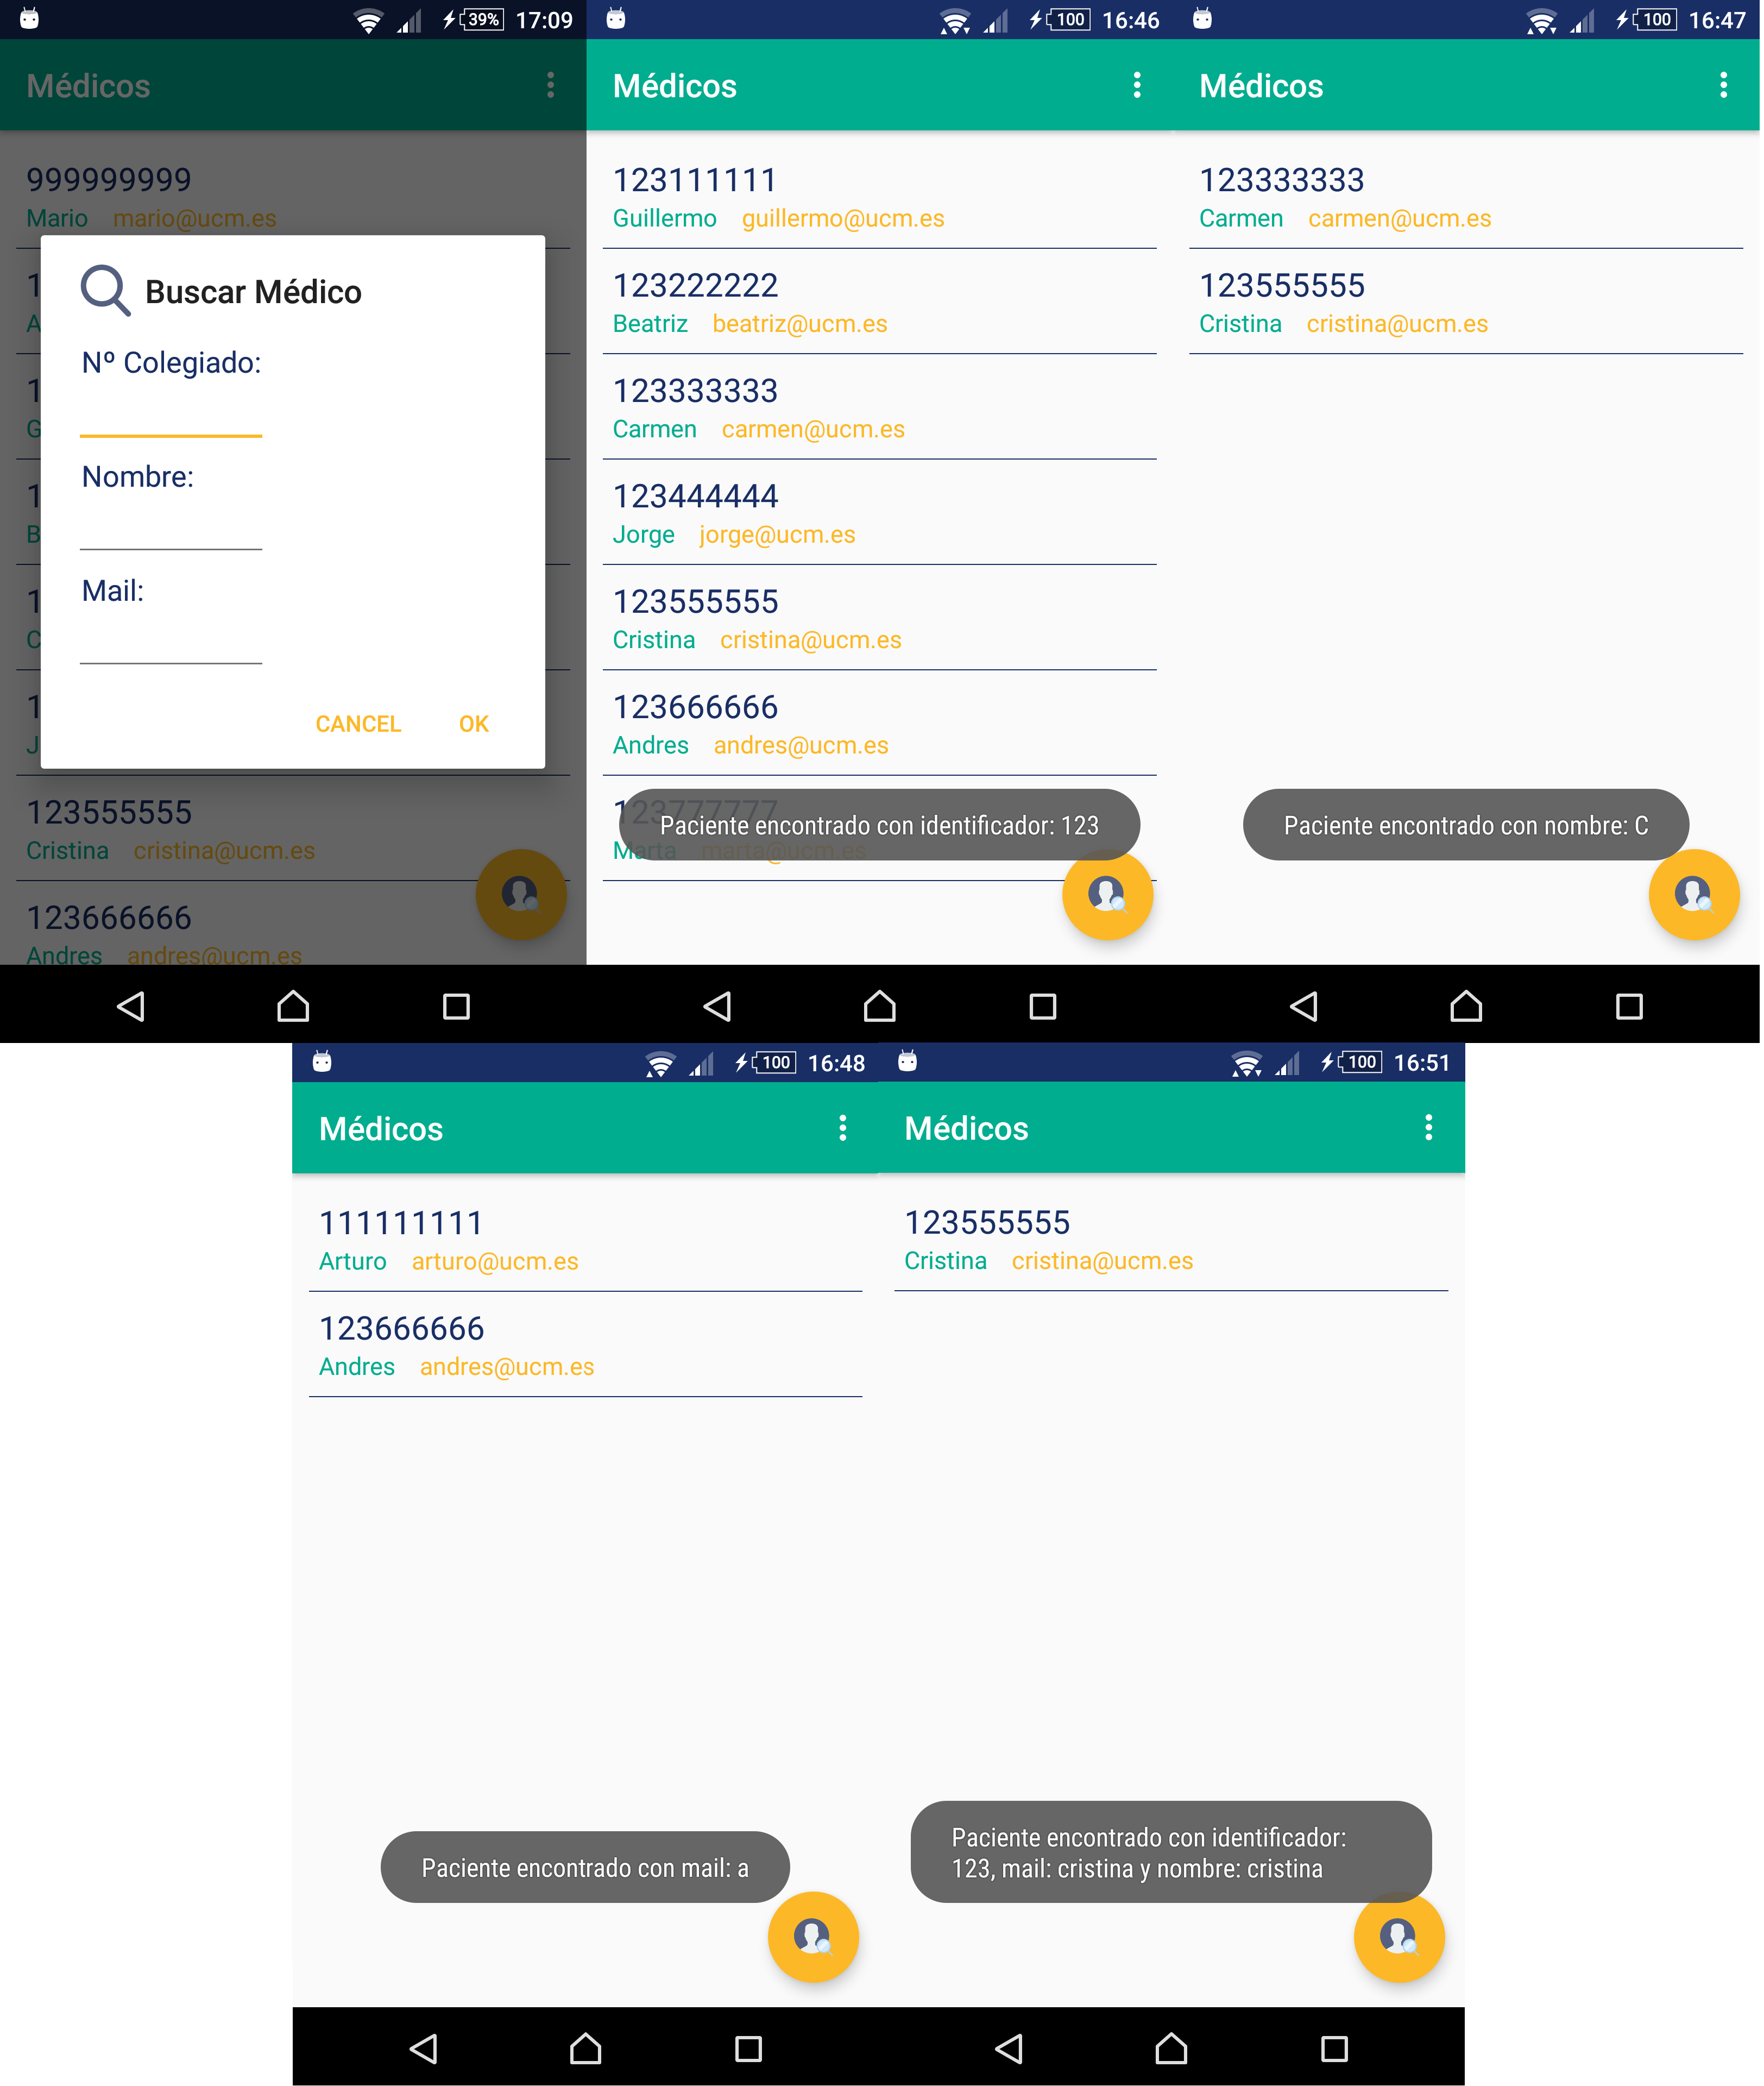
\includegraphics[height= 14cm]{capturas/buscarMedicoFull.png}
\caption{Ventana -  Buscar Aspirante}
\end{figure}

\newpage
\begin{figure}[H]
\centering
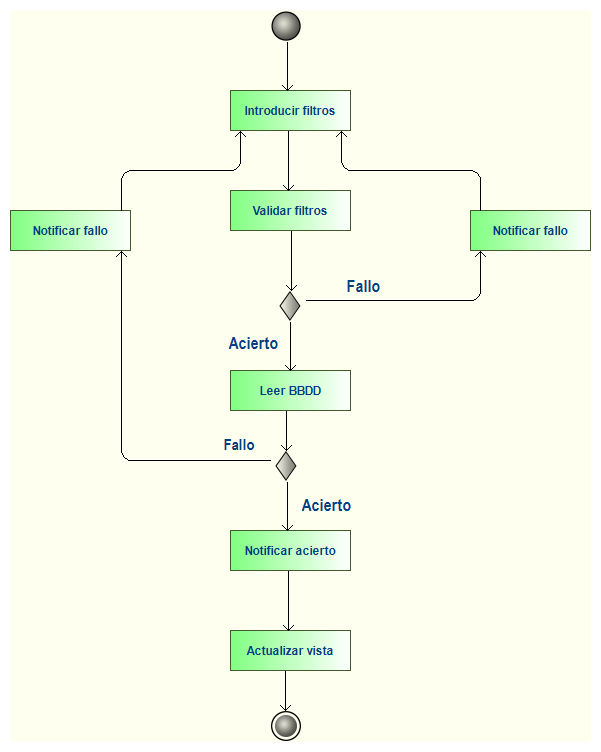
\includegraphics[height= 11cm]{diagramas/BuscarmedicoActivitydiagram.png}
\caption{Diagrama de actividad -  Buscar Aspirante}
\end{figure}

\vfill
%CONSULTAR ASPIRANTE
\subsection {Consultar aspirante}

Al interactuar con un elemento de la lista de aspirantes, al administrador se le guía a otra ventana donde puede consultar una documentación más detallada sobre el candidato (Figura 2.15). A través de esta interfaz, el médico podrá finalmente validarle o removerle en función de si sus datos son fidedignos o no. (Figura 2.16)

\begin{figure}[H]
\centering
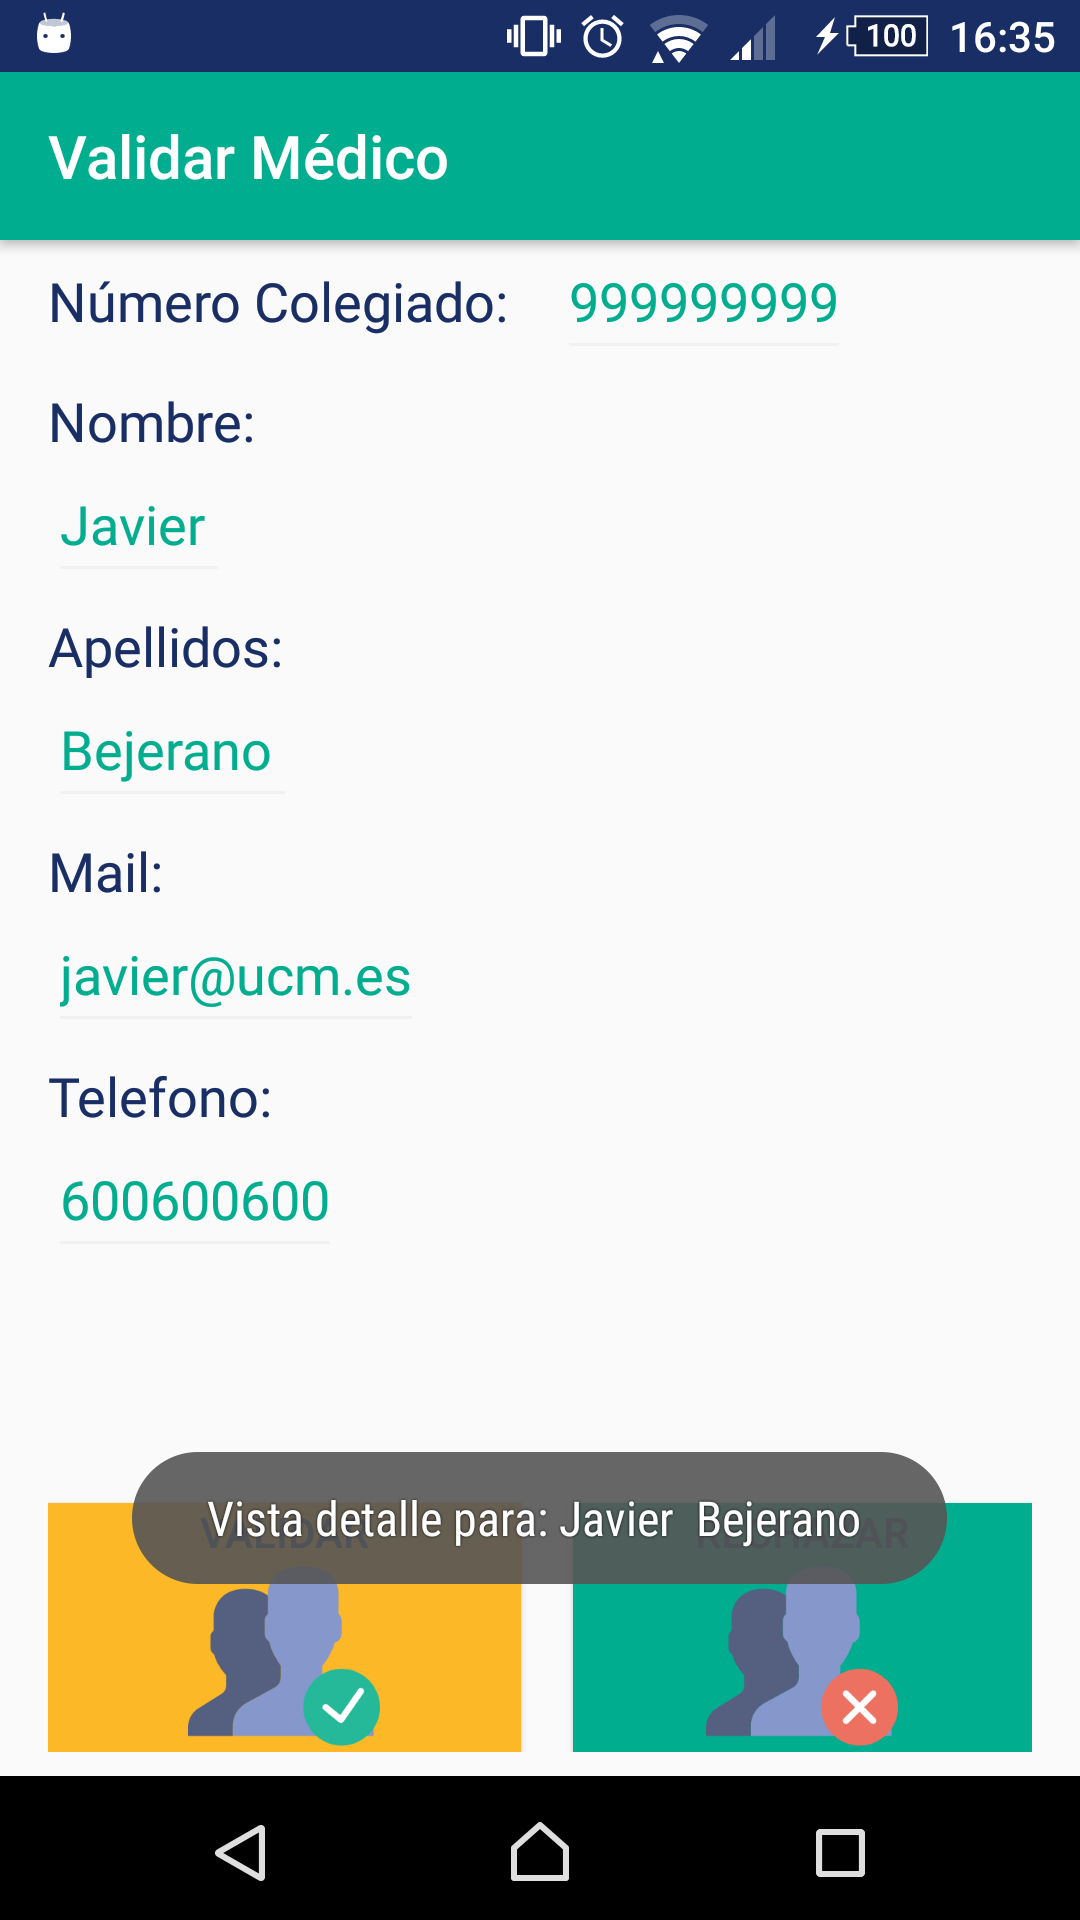
\includegraphics[height= 7cm]{capturas/consultar_medico.png}
\caption{Ventana -  Consultar Aspirante}
\end{figure}

\begin{figure}[H]
\centering
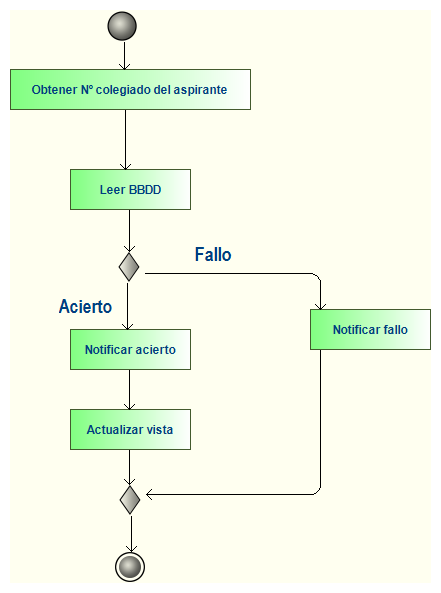
\includegraphics[height= 11cm]{diagramas/ConsultarmedicoActivitydiagram.png}
\caption{Diagrama de actividad -  Consultar Aspirante}
\end{figure}

\vfill
%VALIDAR ASPIRANTE
\subsection {Validar aspirante}

A continuación, presentamos el resultado obtenido al pulsar el botón \textquotedbl Validar\textquotedbl{} en la ventana anterior (Figura 2.15). La aplicación confirmará los datos del solicitante y regresará a la lista de aspirantes donde el usuario será informado del éxito de su operación con un mensaje (Figura 2.17). A partir de este momento, el solicitante podrá acceder a su cuenta e interactuar con lo que ofrece la app. (Figura 2.18)

\begin{figure}[H]
\centering
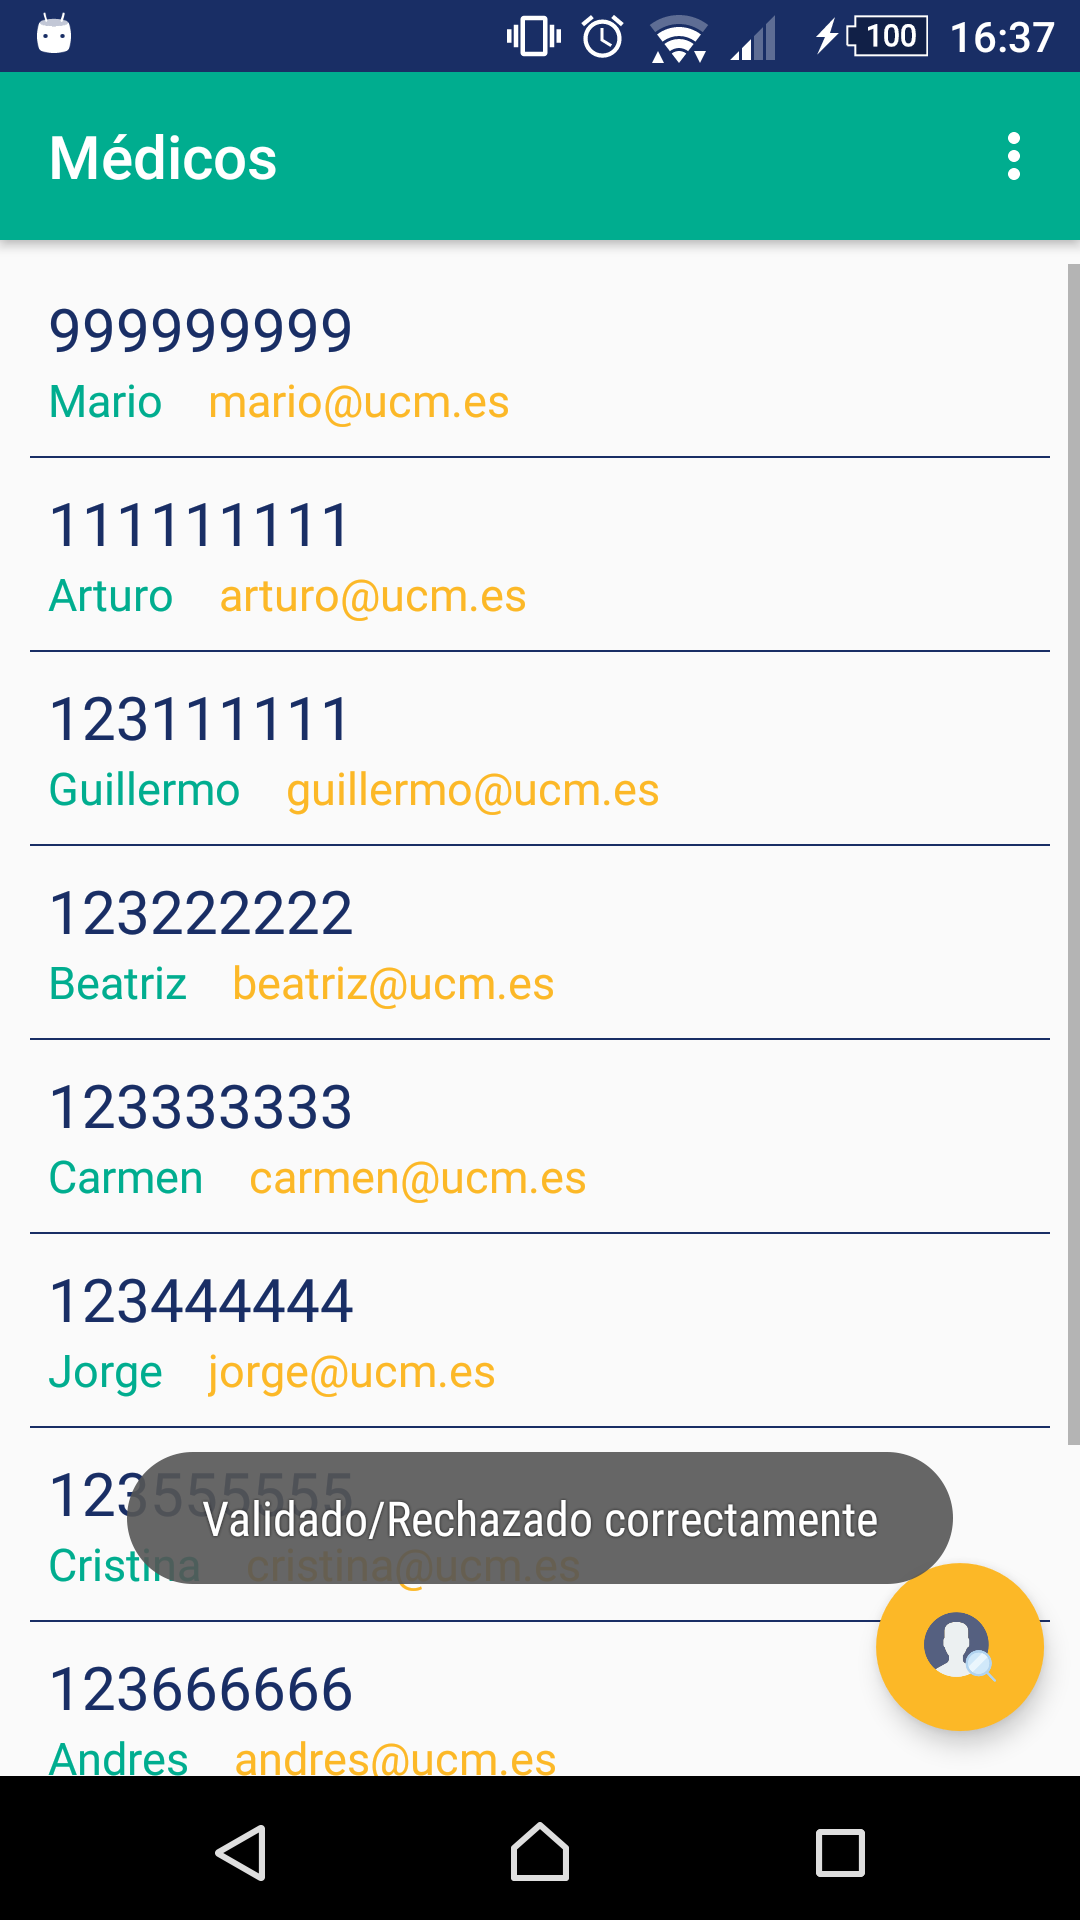
\includegraphics[height= 7cm]{capturas/validar_medico.png}
\caption{Ventana -  Validar Aspirante}
\end{figure}

\begin{figure}[H]
\centering
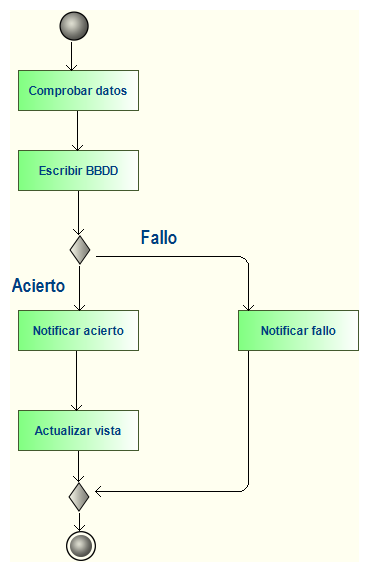
\includegraphics[height= 11cm]{diagramas/ValidarmedicoActivitydiagram.png}
\caption{Diagrama de actividad -  Validar Aspirante}
\end{figure}

\vfill
%RECHAZAR ASPIRANTE
\subsection {Rechazar aspirante}

Si por el contrario el individuo presiona el botón rechazar, la candidatura actual será revocada y todos los datos relativos a ese registro serán removidos (Figura 2.19). (Figura 2.20)

\begin{figure}[H]
\centering
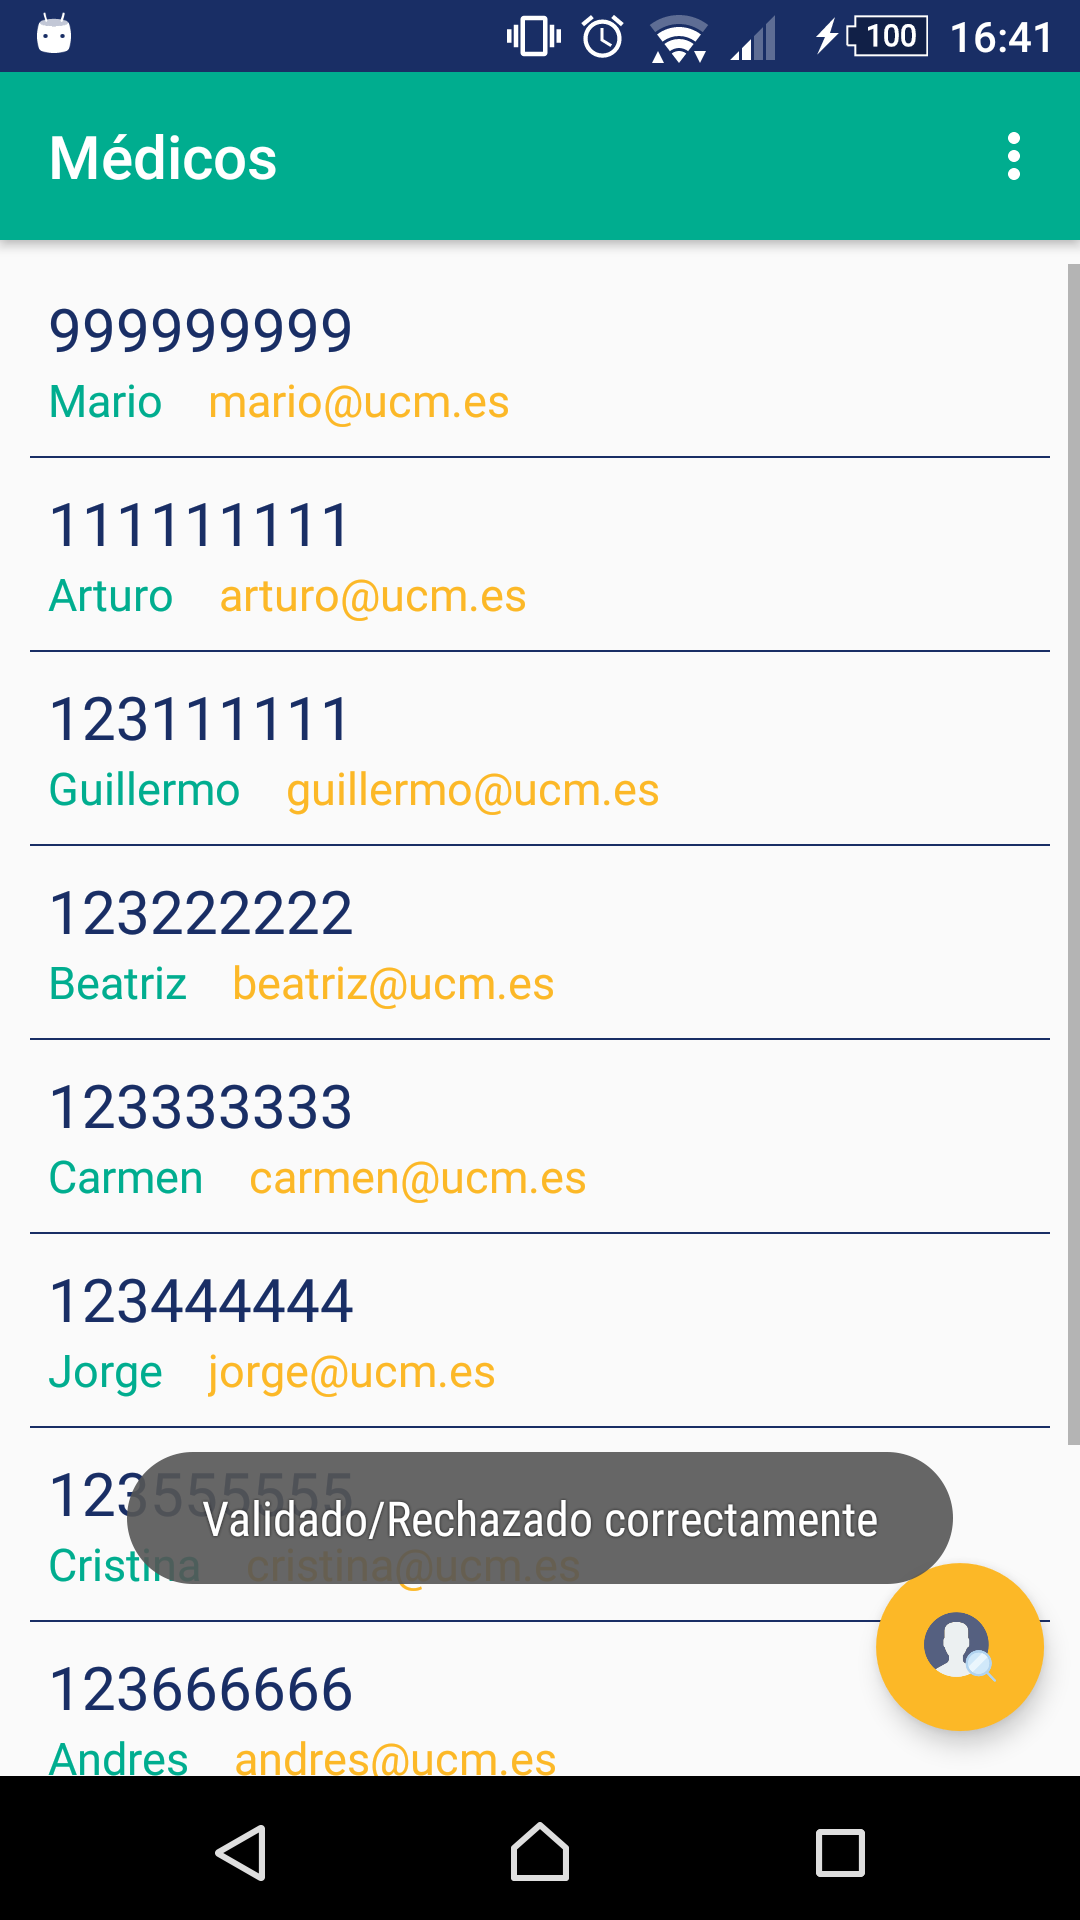
\includegraphics[height= 7cm]{capturas/rechazar_medico.png}
\caption{Ventana -  Rechazar Aspirante}
\end{figure}

\begin{figure}[H]
\centering
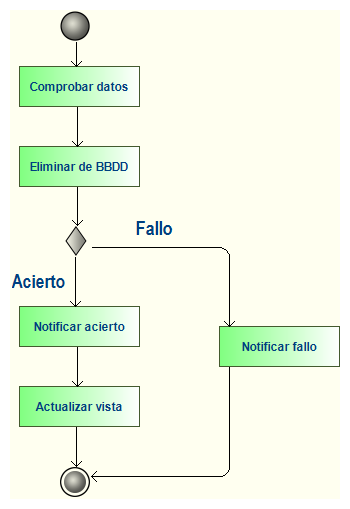
\includegraphics[height= 11cm]{diagramas/RechazarmedicoActivitydiagram.png}
\caption{Diagrama de actividad -  Rechazar Aspirante}
\end{figure}

\vfill
%%%%%%%%%%%%COMUNES
\section {Facultades comunes a ambos perfiles}

Existen situaciones compartidas por ambos tipos de usuario. El proceso de registro y acceso de los usuarios a su cuenta, la consulta y alteración de datos de un paciente y los filtros de búsqueda para los resultados de una lista son ejemplos de estos casos.

%INICIO DE SESION
\subsection {Inicio de sesión}

Cuando ejecutamos la aplicación nos aparece el login, el cual nos permite autentificar nuestras credenciales para acceder a nuestra cuenta. Se nos requerirá el número de colegiado y la contraseña (Figura 2.21).
Si no dispones de una cuenta puedes solicitar registro mediante el botón de la parte inferior. Esta funcionalidad se explica en detalle en el siguiente punto. (Figura 2.22)

\begin{figure}[H]
\centering
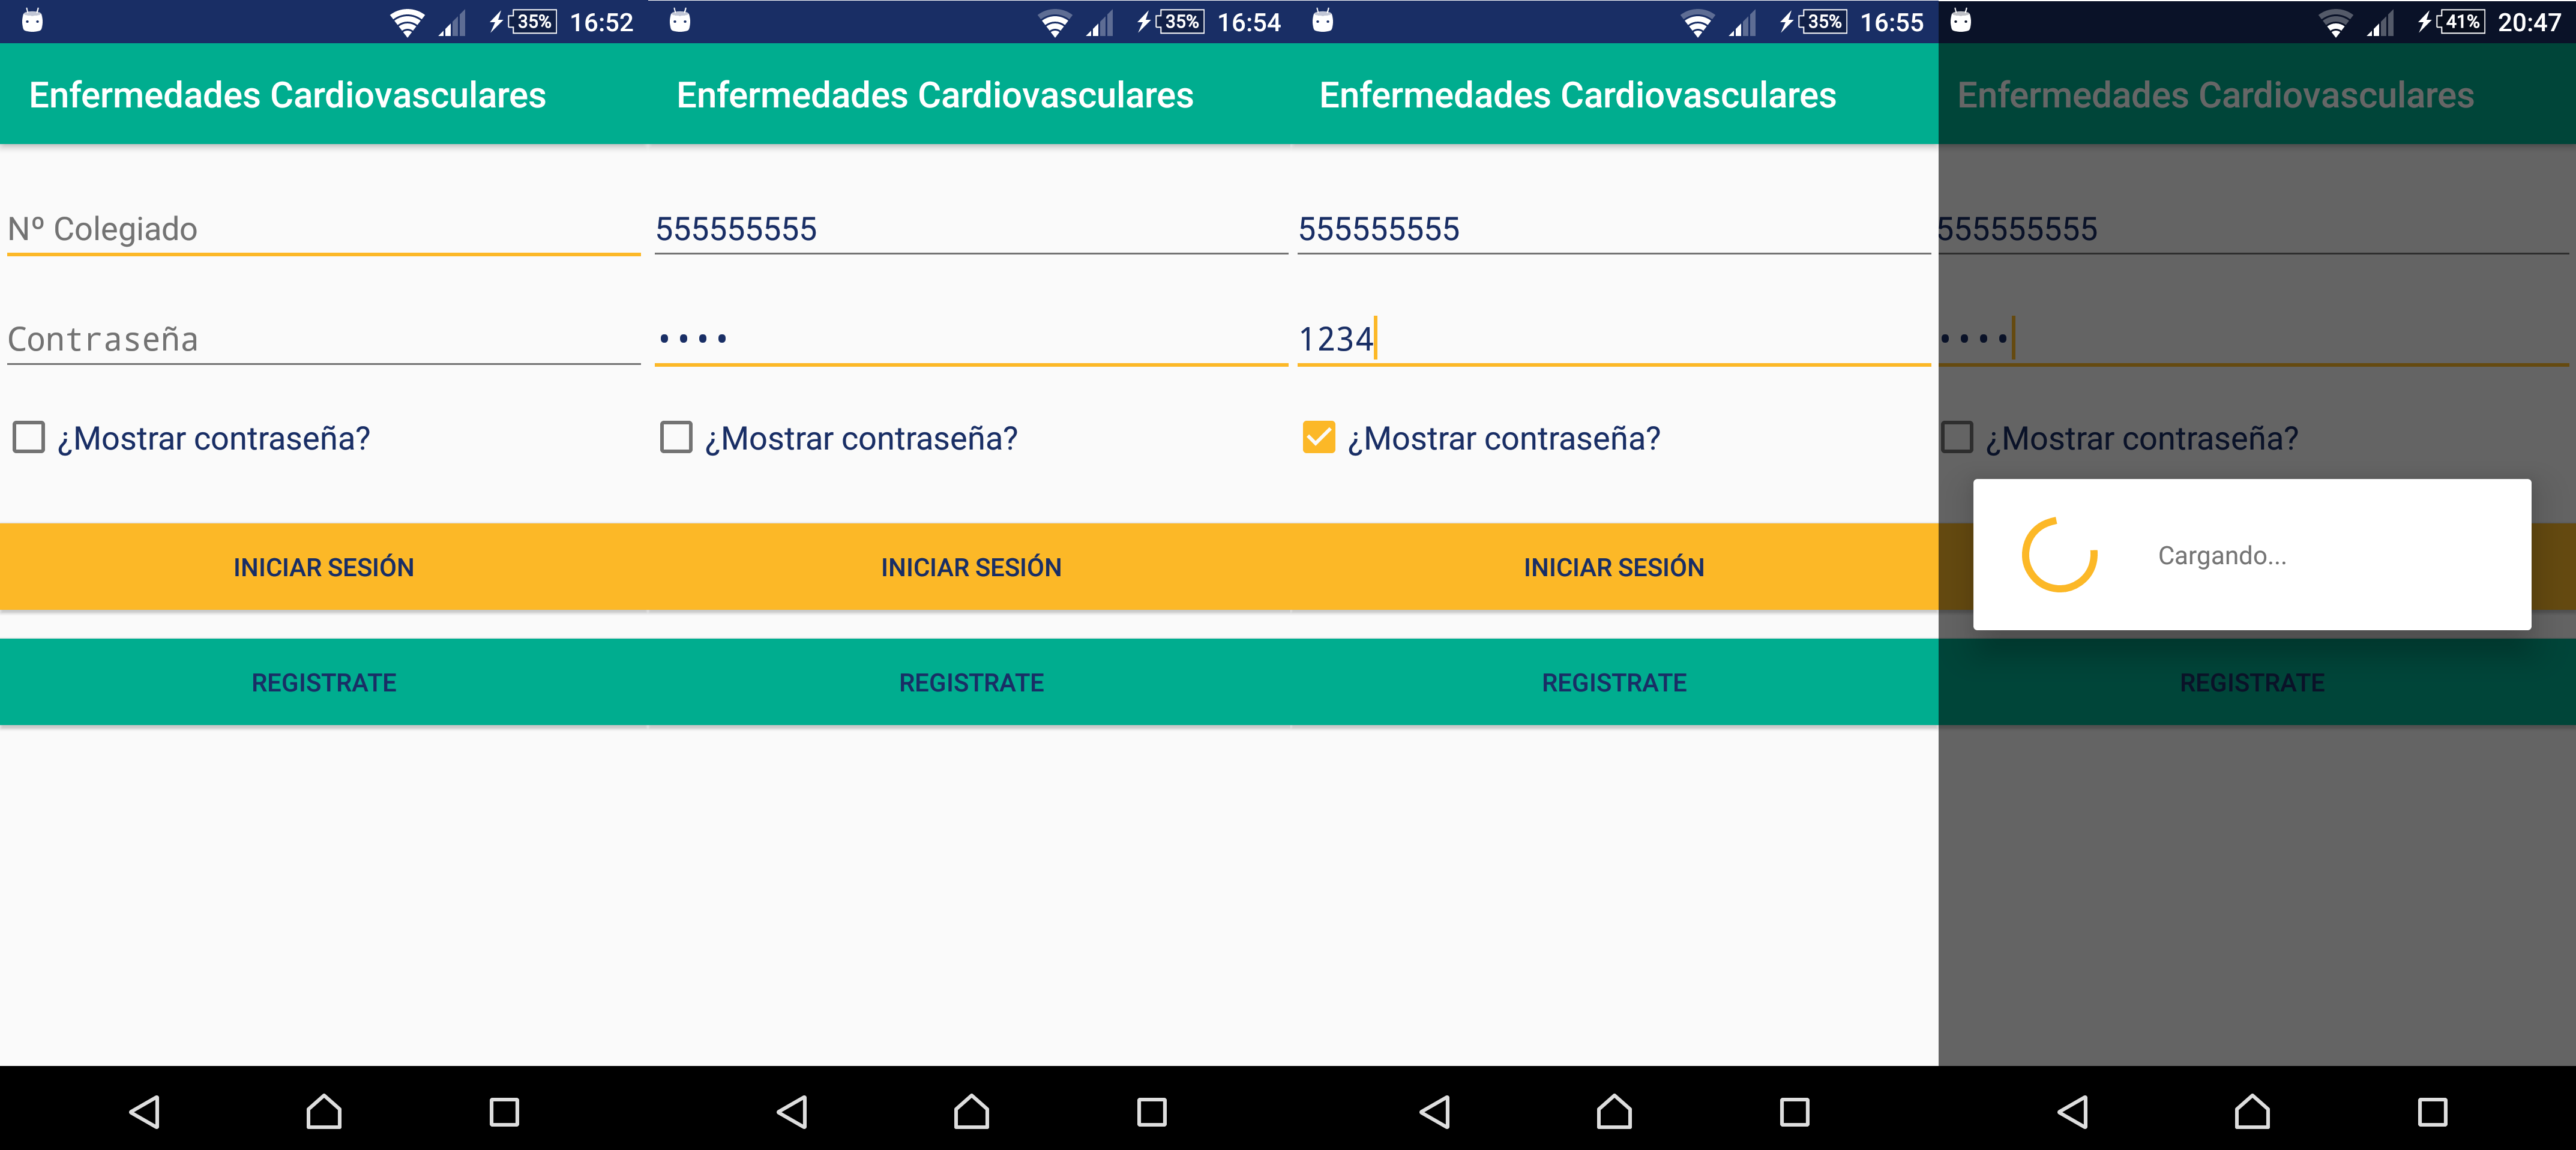
\includegraphics[height=6.7cm]{capturas/logIn.png}
\caption{Ventana - Inicio de sesión}
\end{figure}

\newpage
\begin{figure}[H]
\centering
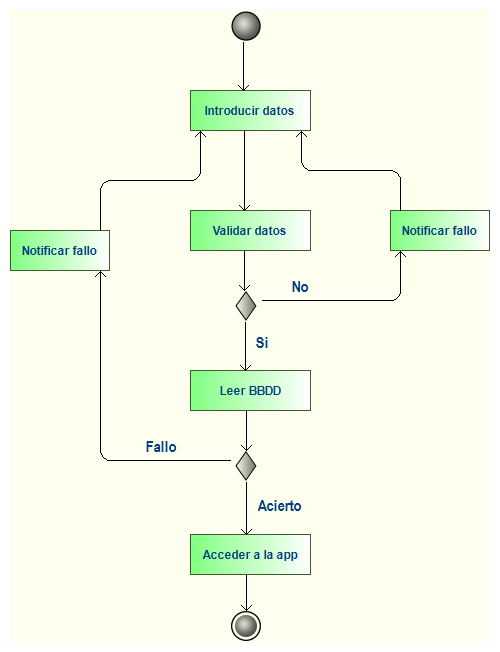
\includegraphics[height= 11cm]{diagramas/LoginActivitydiagram.png}
\caption{Diagrama de actividad - Inicio Sesión}
\end{figure}

\newpage
%REGISTRO
\subsection {Registro}

Si el solicitante desea adquirir una cuenta como médico pueden introducir sus datos en esta ventana. La aplicación requiere el nombre y apellidos, el número de colegiado que identifica al profesional sanitario, la dirección de correo electrónico, el teléfono de contacto y la contraseña que se va utilizar posteriormente para tener acceso a su cuenta en la aplicación (Figura 2.23). Todos los campos mencionados son obligatorios y se comprobará que los datos introducidos son válidos.
La aplicación notificará el éxito o fracaso de la operación, resaltando los fallos específicos ocurridos en este último caso. (Figura 2.24)

\begin{figure}[H]
\centering
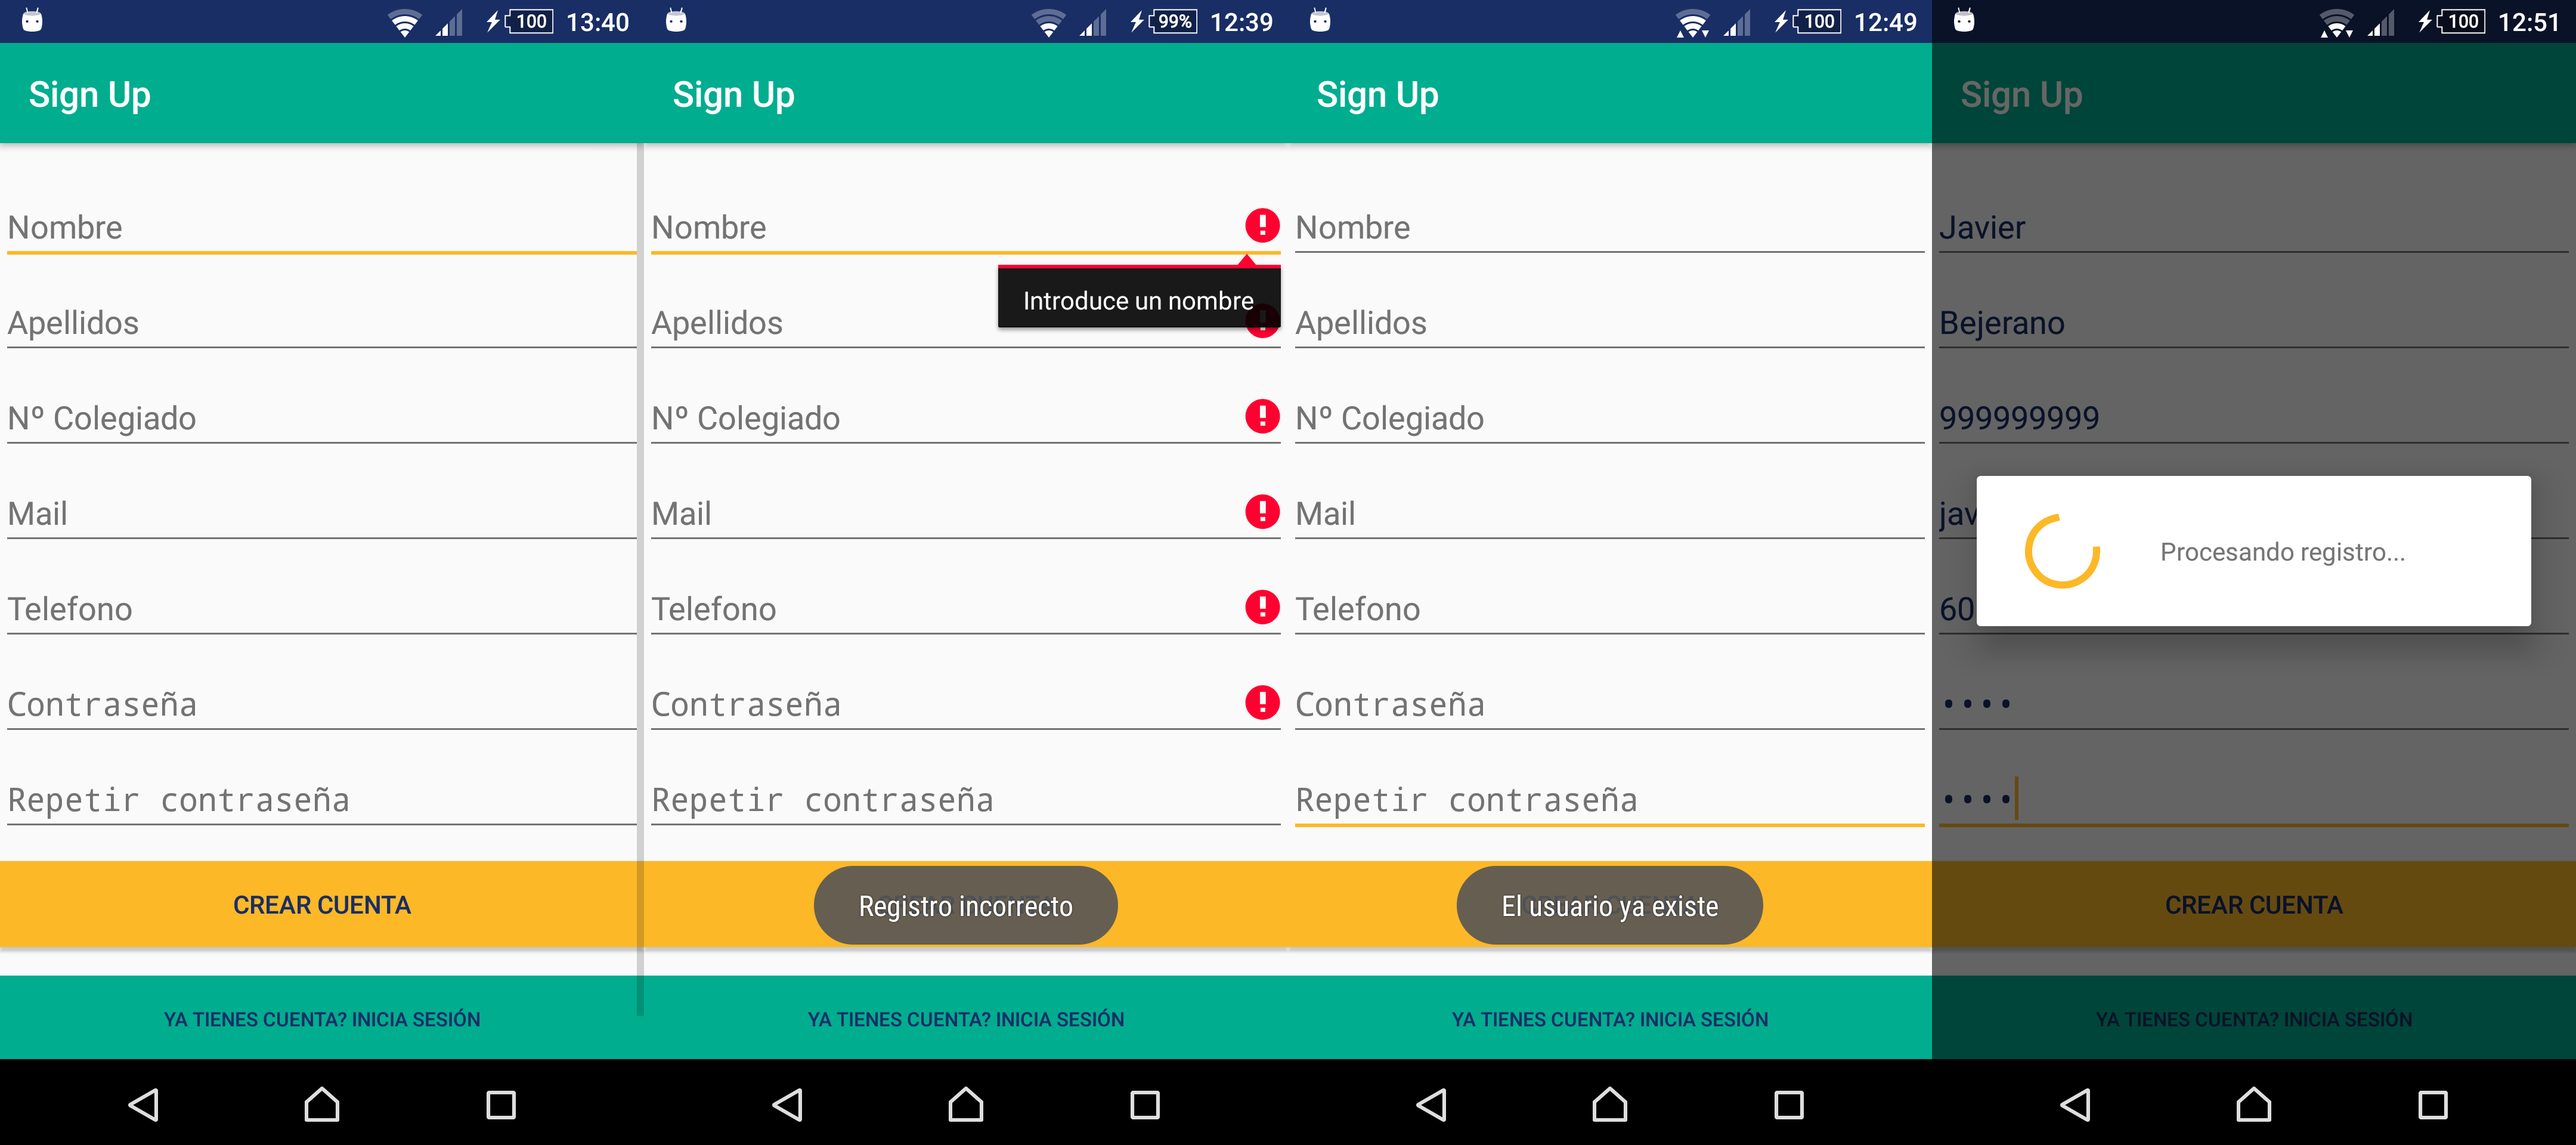
\includegraphics[height= 6.7cm]{capturas/sign_upFull.png}
\caption{Ventana - Registro}
\end{figure}

\newpage
\begin{figure}[H]
\centering
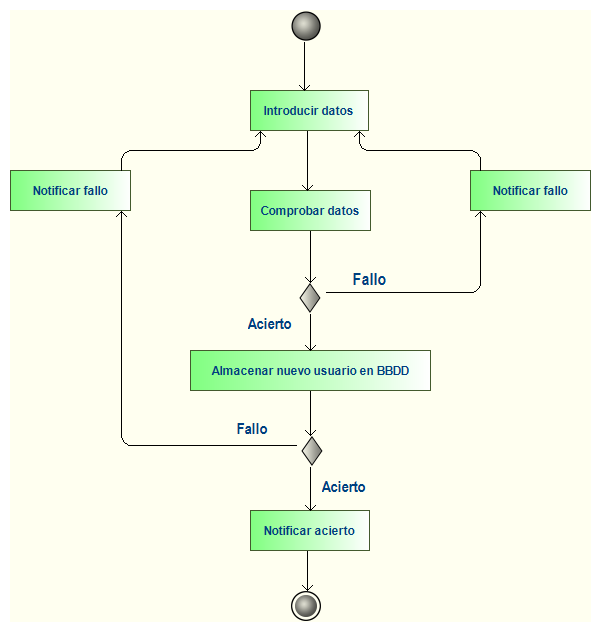
\includegraphics[height= 11cm]{diagramas/SignupActivitydiagram.png}
\caption{Diagrama de actividad - Registro}
\end{figure}

\newpage
%MIS PACIENTES
\subsection {Mis pacientes}

Visualiza una lista con la información básica de tus pacientes, a saber, el ID, la edad y el género (M: Masculino, F: Femenino) (Figura 2.25). Se ofrece la posibilidad de buscar haciendo uso del botón flotante de la parte inferior, así como compartir un paciente con otro médico manteniendo presionado su información asociada en la lista. Ambas posibilidades se describirán en profundidad posteriormente. (Figura 2.26)

\begin{figure}[H]
\centering
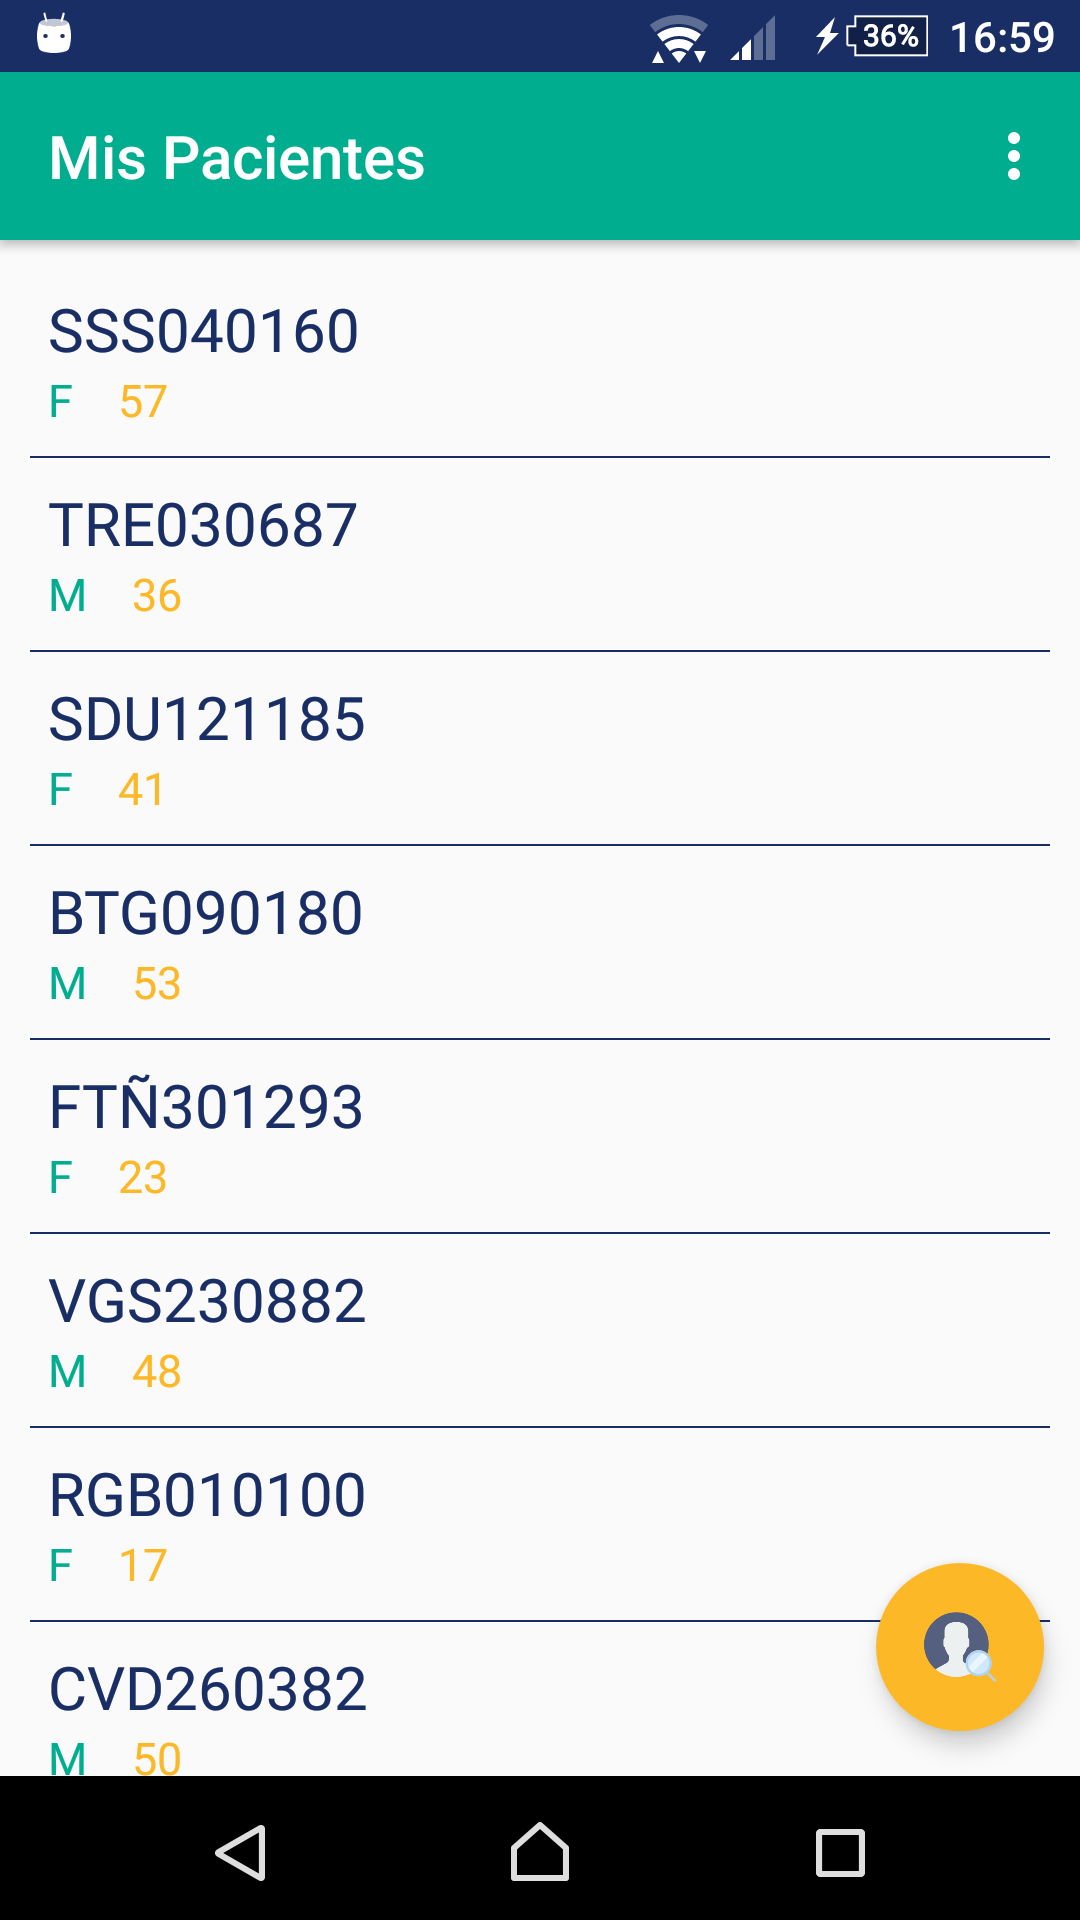
\includegraphics[height= 7cm]{capturas/mis_pacientes.png}
\caption{Ventana - Mis Pacientes}
\end{figure}

\begin{figure}[H]
\centering
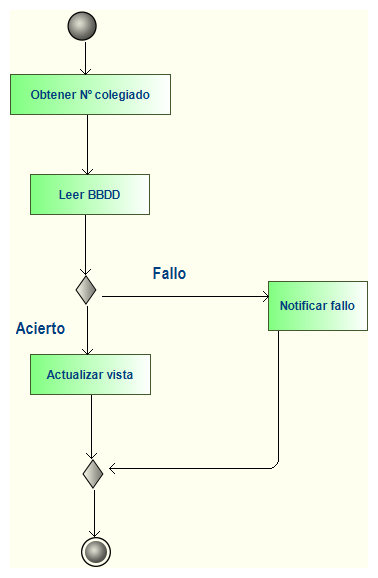
\includegraphics[height= 11cm]{diagramas/ListapacientesActivitydiagram.png}
\caption{Diagrama de actividad - Mis Pacientes}
\end{figure}

%COMPARTIR PACIENTE
\subsection {Compartir paciente}

La aplicación permite que un paciente sea tratado simultáneamente  por más de un médico. En esta ventana emergente el usuario introduce el número de colegiado del médico con el que quiere compartir los datos del paciente (Figura 2.27). Tras esta acción, este último quedará reflejado en la lista de pacientes del otro médico. (Figura 2.28)

\begin{figure}[H]
\centering
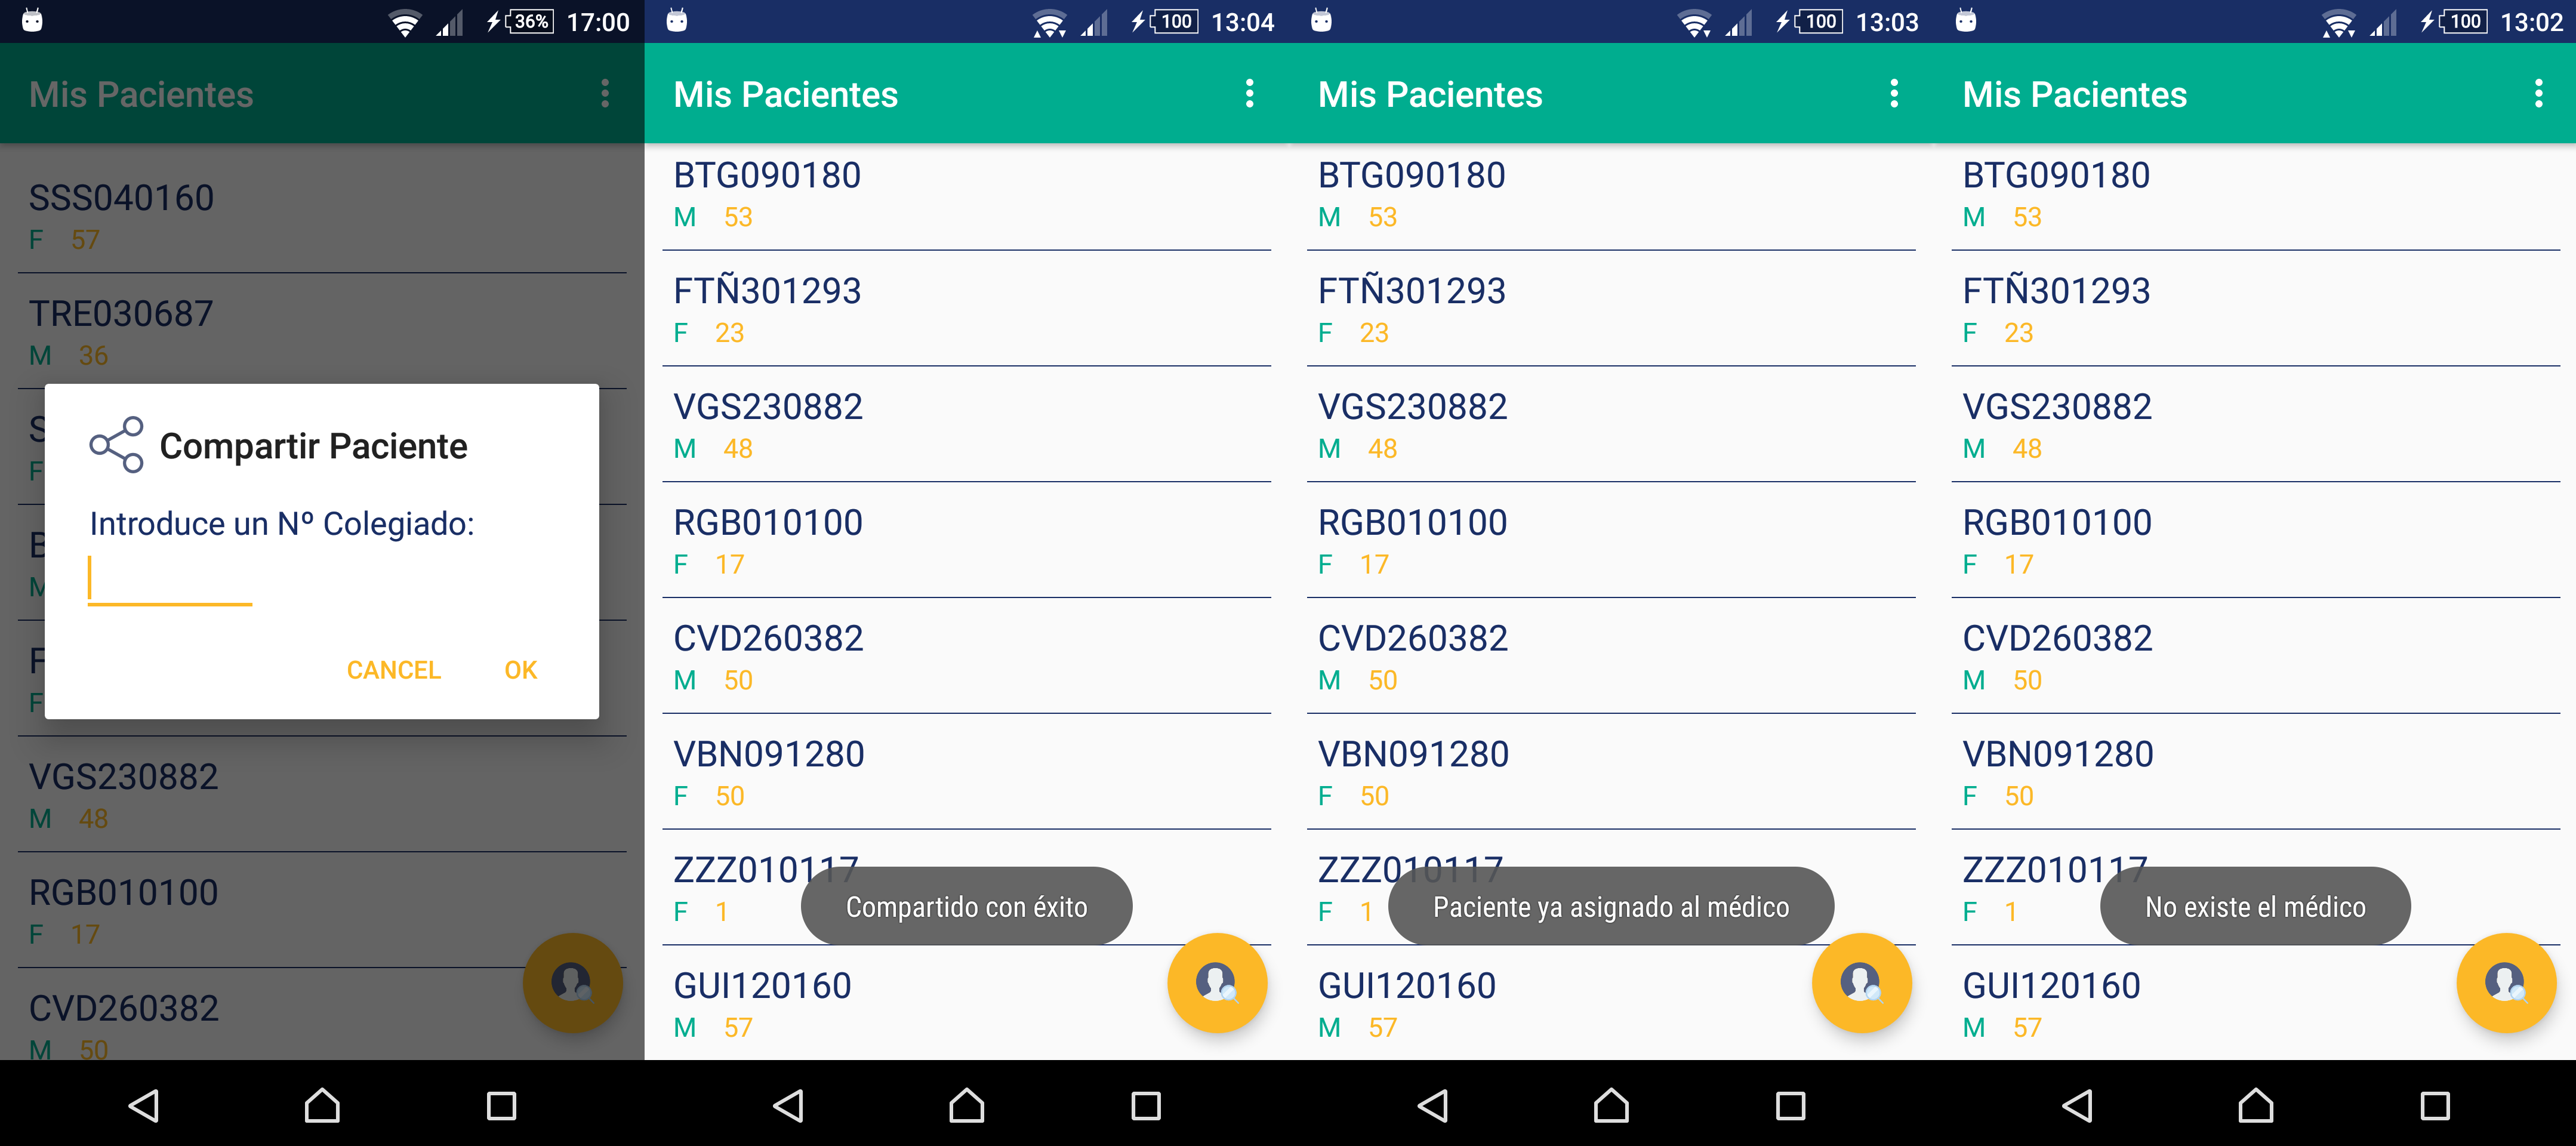
\includegraphics[height= 6.7cm]{capturas/compartir_pacienteFull.png}
\caption{Ventana - Compartir Paciente}
\end{figure}

\begin{figure}[H]
\centering
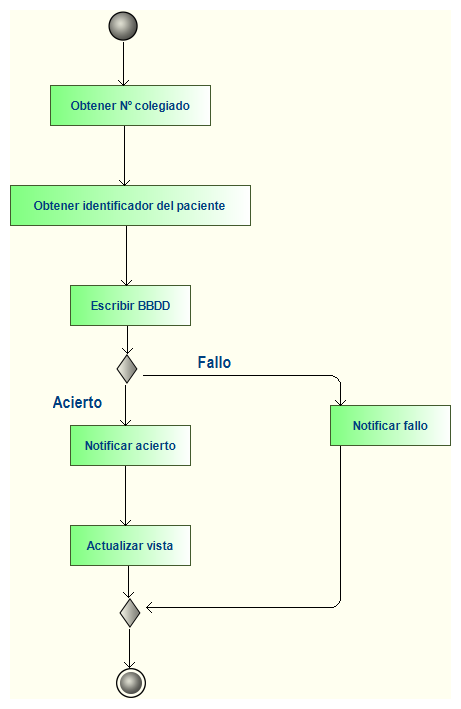
\includegraphics[height= 11cm]{diagramas/CompartirpacienteActivitydiagram.png}
\caption{Diagrama de actividad - Compartir Paciente}
\end{figure}

\newpage
%BUSCAR PACIENTE
\subsection {Buscar paciente}

Para evitar las demoras de una lista con una gran cantidad de pacientes se facilita una serie filtros que permite encontrar con mayor facilidad al paciente(s) deseado(s). Se puede realizar una búsqueda  por identificador (parcial o completo), género, edad o una combinación entre ellos (Figura 2.29). La aplicación informará sobre el resultado y los filtros utilizados. Un caso particular es el de la ausencia de filtros, que resultará en la obtención de todos los pacientes. (Figura 2.30)

\begin{figure}[H]
\centering
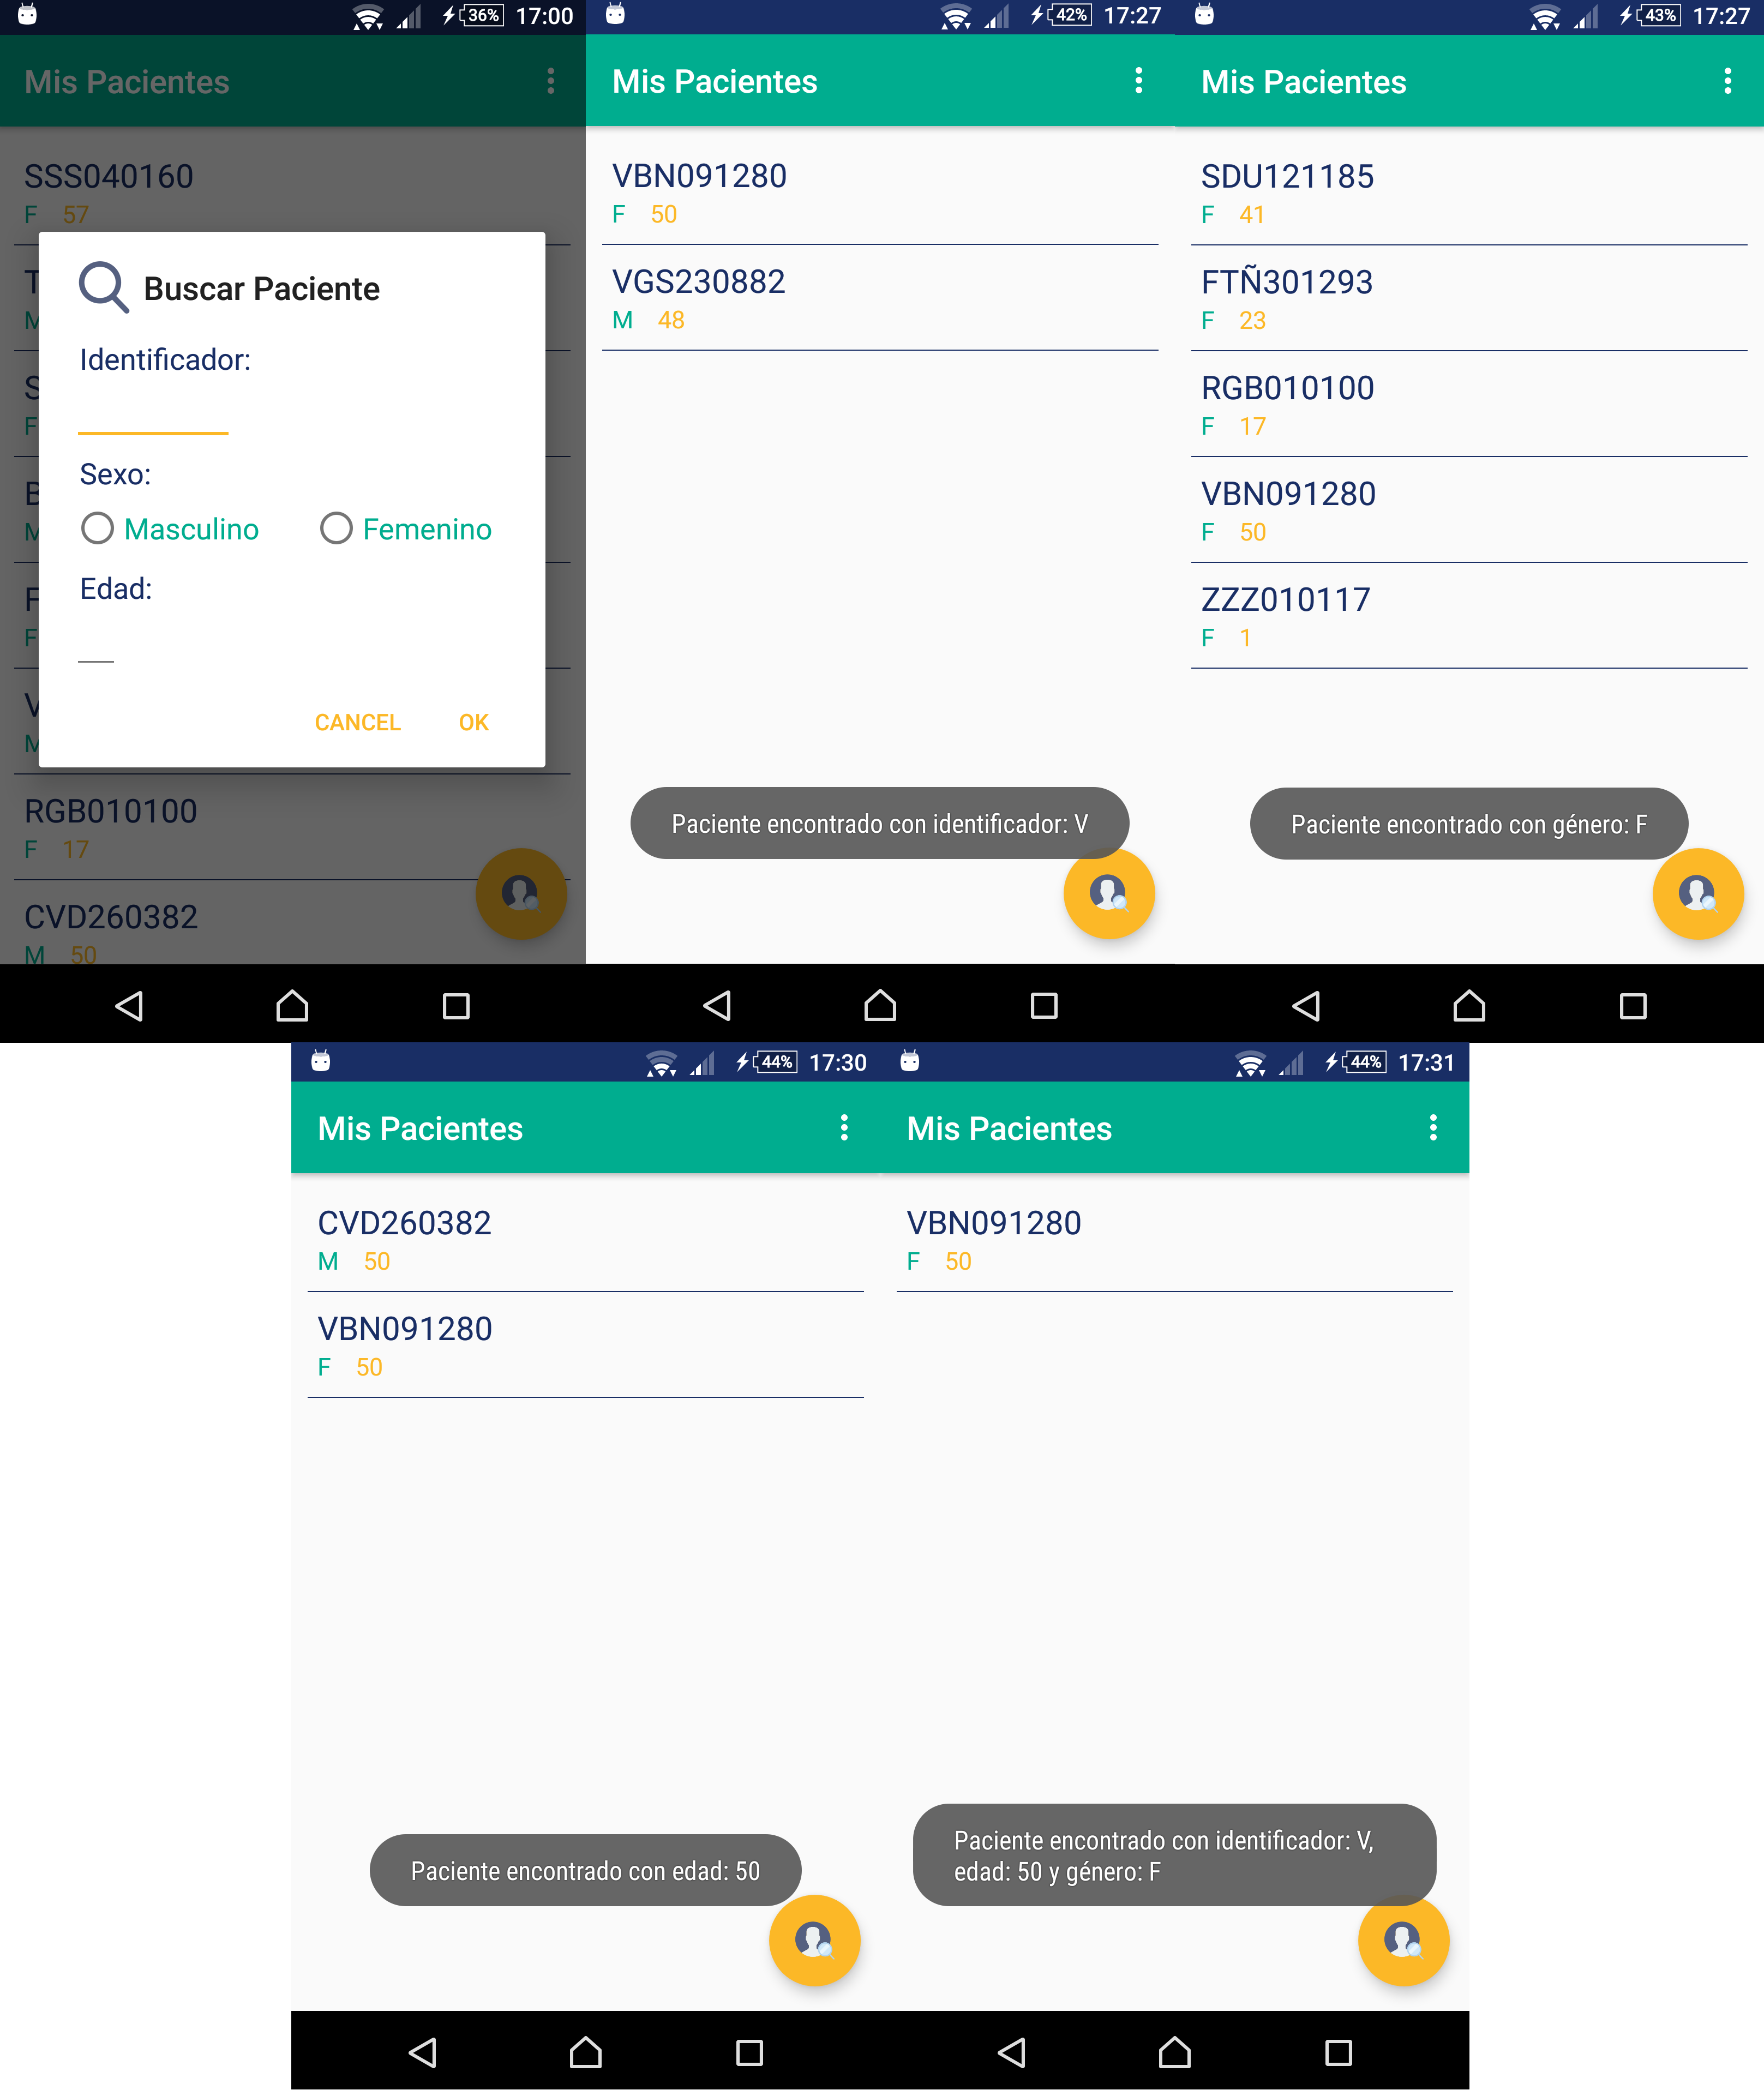
\includegraphics[height= 14cm]{capturas/buscarPacienteFull.png}
\caption{Ventana - Buscar Paciente}
\end{figure}

\newpage
\begin{figure}[H]
\centering
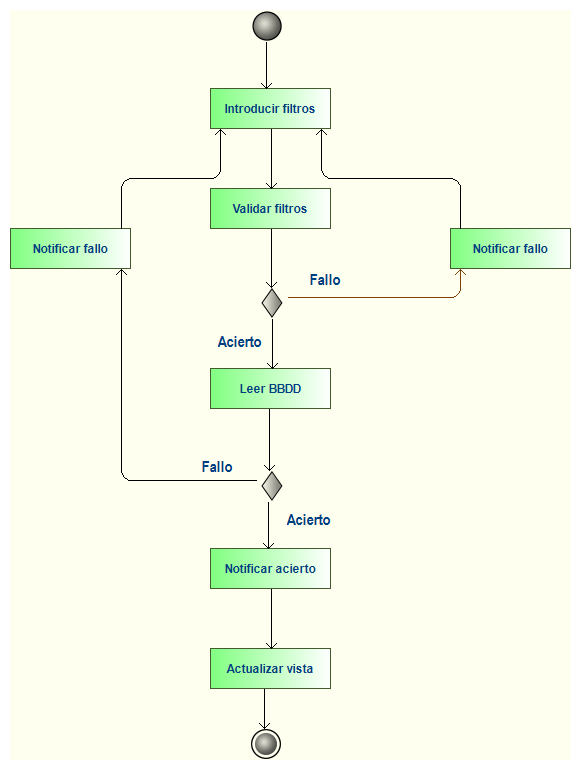
\includegraphics[height= 11cm]{diagramas/BuscarpacienteActivitydiagram.png}
\caption{Diagrama de actividad - Buscar Paciente}
\end{figure}

\newpage
%CONSULTAR PACIENTE
\subsection {Consultar paciente}

En el caso de que se introduzcan datos erróneos en el alta del paciente o se desee actualizar la información del mismo, la app posibilita alterar dichos datos en esta ventana (Figura 2.31). También es posible eliminar al paciente de su lista personal. Además, sirve de punto de partida para las funcionalidades consistentes en calcular su riesgo cardiovascular, establecer el tratamiento y/o descargar el informe de su estado en formato PDF. (Figura 2.32, Figura 2.33 y Figura 2.34)

\begin{figure}[H]
\centering
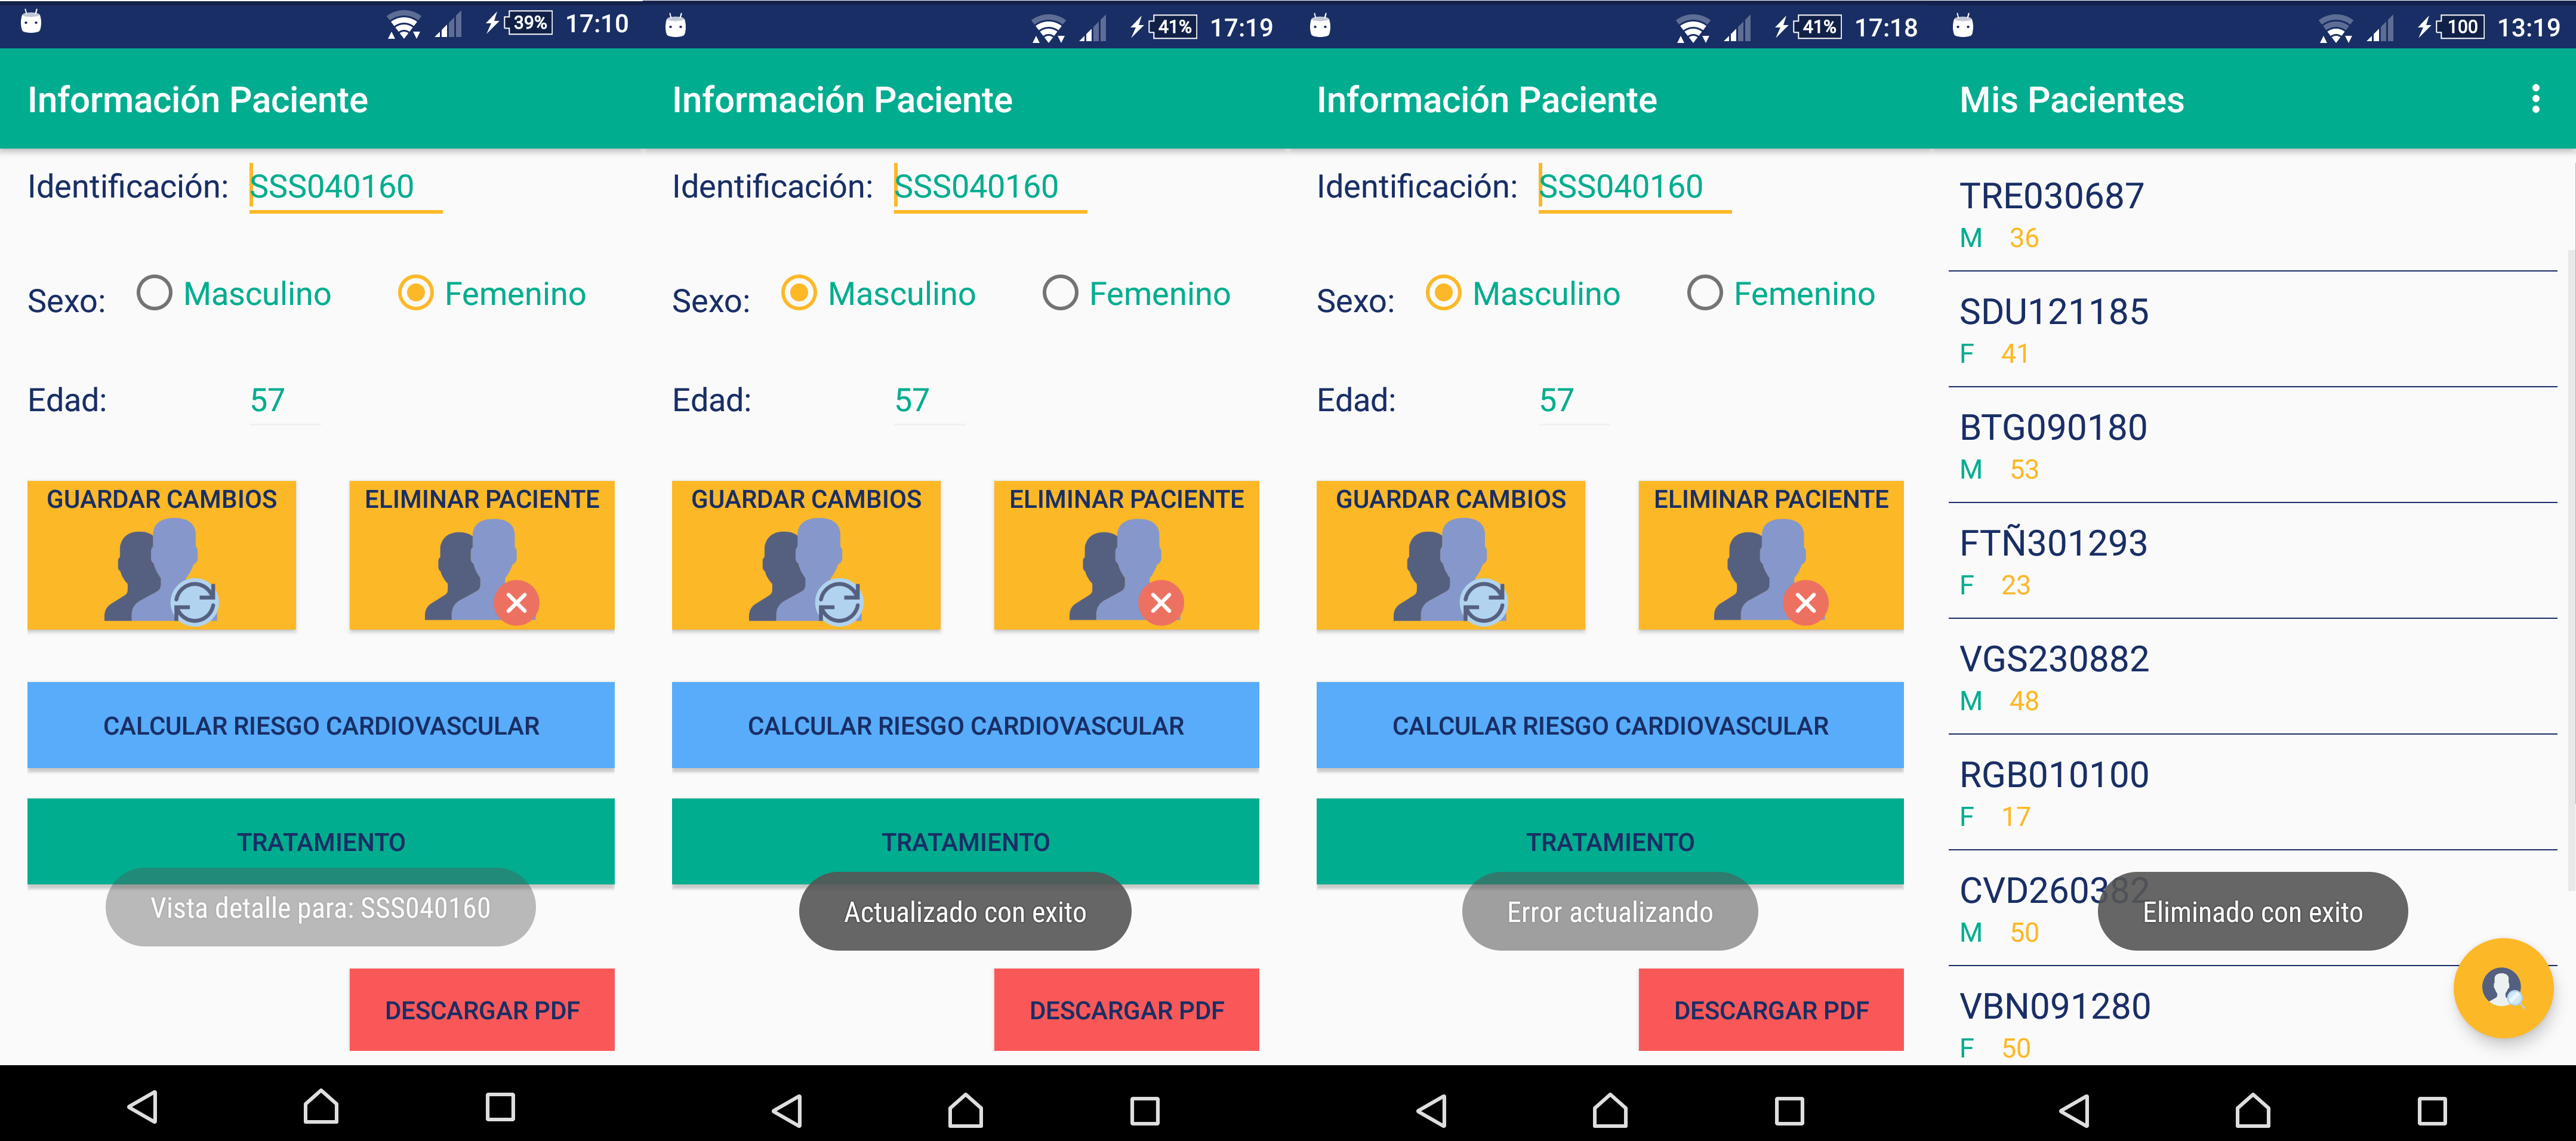
\includegraphics[height= 6.7cm]{capturas/infoPacienteFull2.png}
\caption{Ventana - Consultar Paciente}
\end{figure}

\begin{figure}[H]
\centering
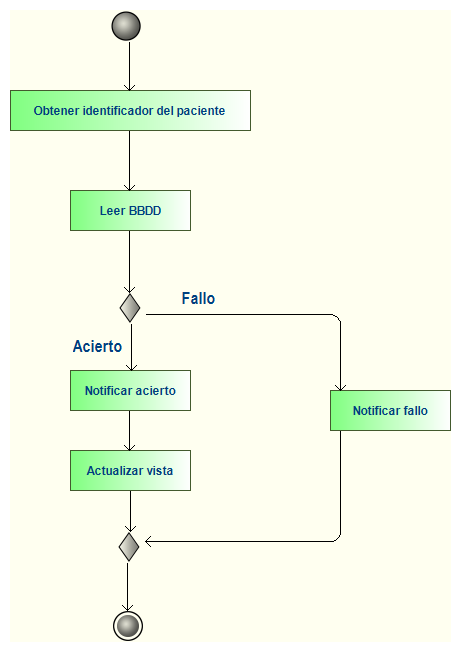
\includegraphics[height= 11cm]{diagramas/ConsultarpacienteActivitydiagram.png}
\caption{Diagrama de actividad - Consultar Paciente}
\end{figure}

\begin{figure}[H]
\centering
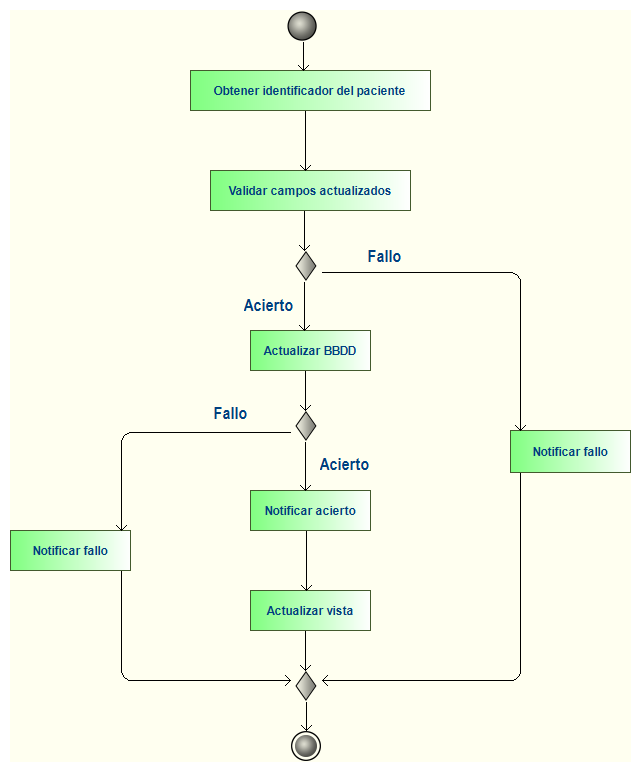
\includegraphics[height= 11cm]{diagramas/ActualizarpacienteActivitydiagram.png}
\caption{Diagrama de actividad - Actualizar Paciente}
\end{figure}

\begin{figure}[H]
\centering
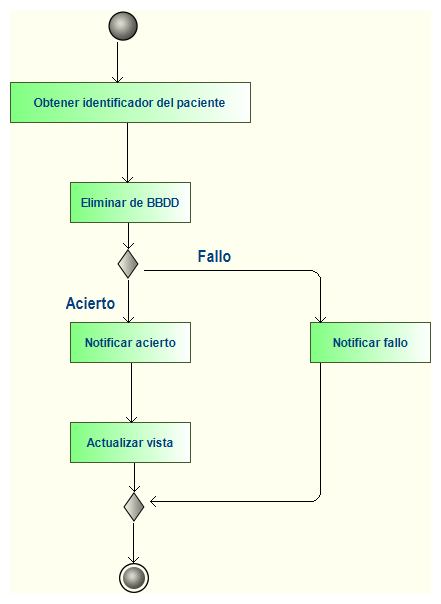
\includegraphics[height= 11cm]{diagramas/EliminarpacienteActivitydiagram.png}
\caption{Diagrama de actividad - Eliminar Paciente}
\end{figure}

%TABAQUISMO
\subsection {Calcular tabaquismo}

El hábito de fumar es uno de los aspectos más determinantes en el cálculo del riesgo cardiovascular. Nuestro fundamento es la fórmula IPA (índice de paquete al año) que se define como (\ref{eq:tabaquismo}):
\begin{equation}\label{eq:tabaquismo}
IPA = \frac{\textup{Cigarrillos por día} * \textup{Años fumando}}{20}
\end{equation}
La pantalla pregunta por las dos entradas (cigarrillos y años) y devuelve el índice IPA calculado (Figura 2.35). De igual forma que en otros casos se anunciará el éxito o fracaso de la operación. (Figura 2.36)

\begin{figure}[H]
\centering
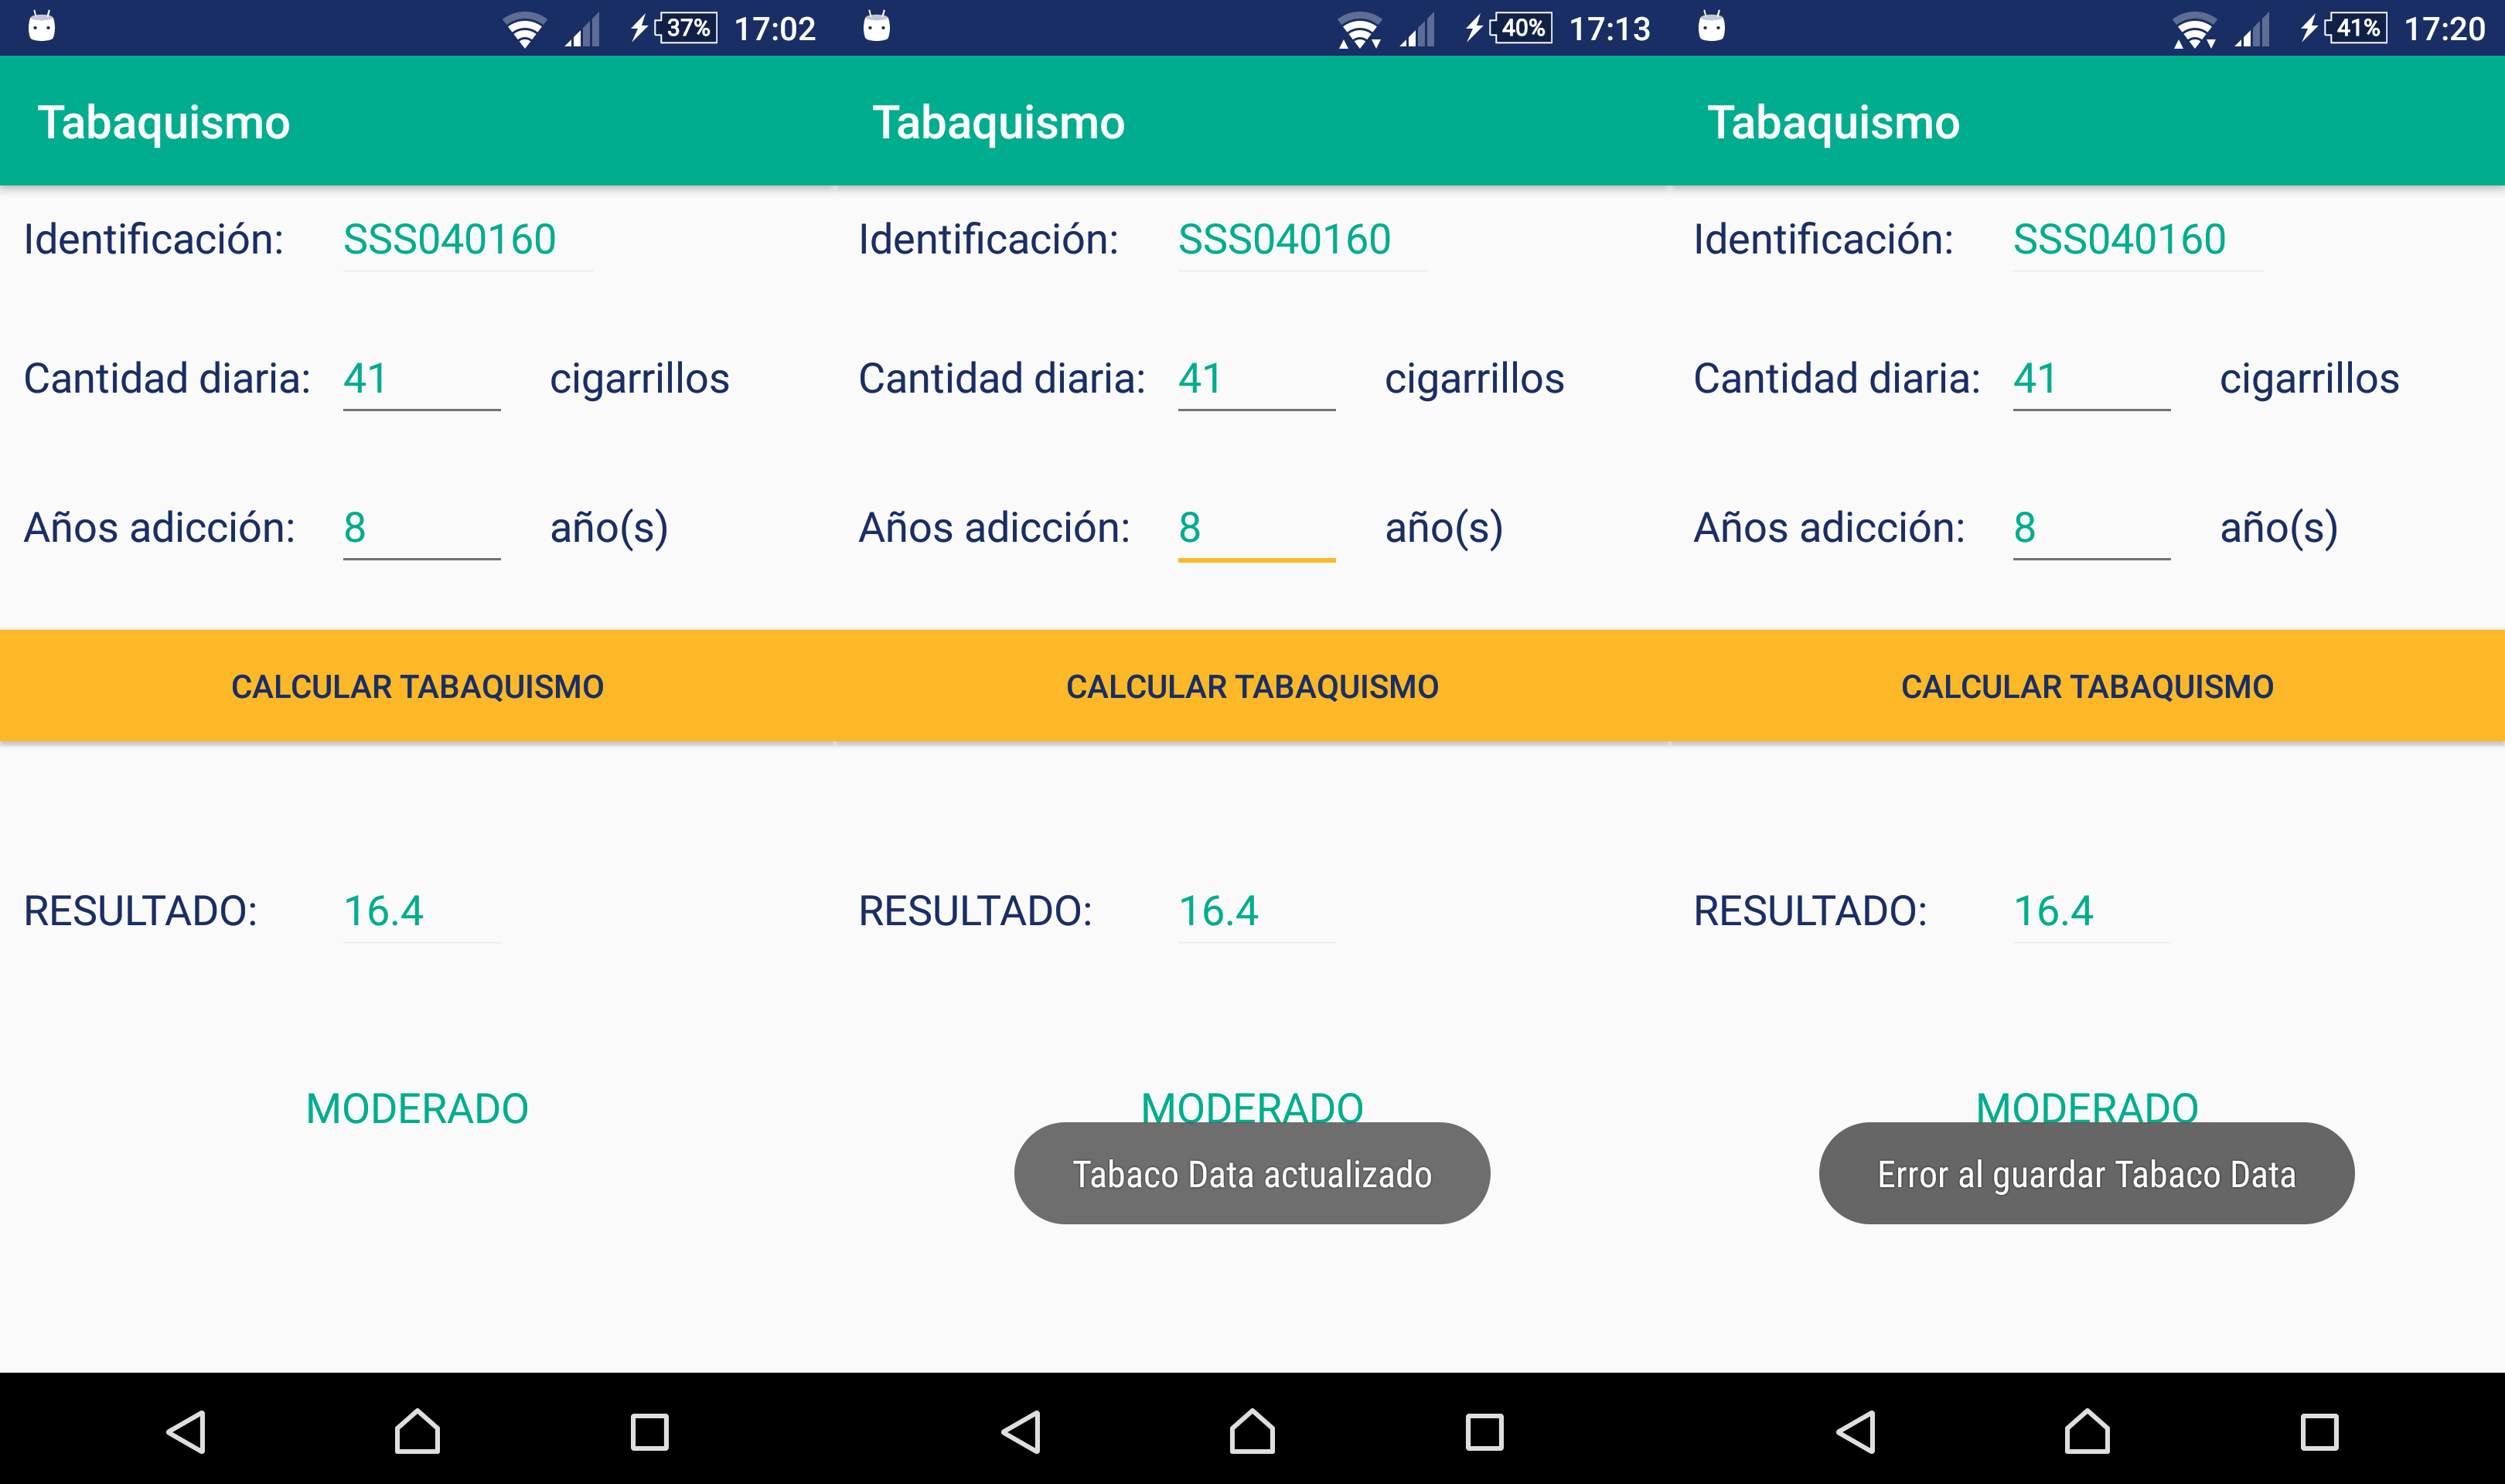
\includegraphics[height= 7cm]{capturas/tabaquismoFull.png}
\caption{Ventana - Tabaquismo}
\end{figure}

\newpage
\begin{figure}[H]
\centering
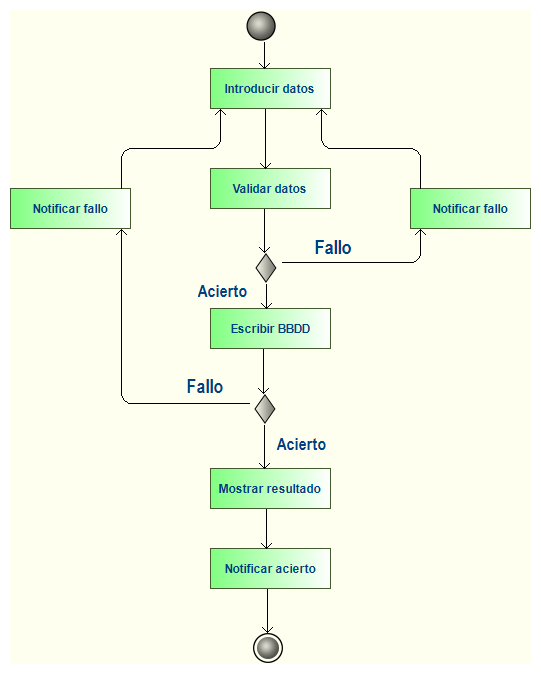
\includegraphics[height= 11cm]{diagramas/TabaquismoActivitydiagram.png}
\caption{Diagrama de actividad - Tabaquismo}
\end{figure}

\newpage
%DIABETES
\subsection {Calcular diabetes}

La diabetes es un esencial entre los causantes de enfermedades cardiovasculares. Por esta razón nuestra app recoge numerosos campos de influencia para que el médico pueda determinar un tratamiento eficaz (Figura 2.37). Los datos solicitados: tipo de diabetes, tratamiento, hemoglobina glucosilada, monitor continuo de glucosa (CGM), años de enfermedad, fecha último fondo de ojos, creatinina, microalbuminuria, urea y raza. (Figura 2.38)

\begin{figure}[H]
\centering
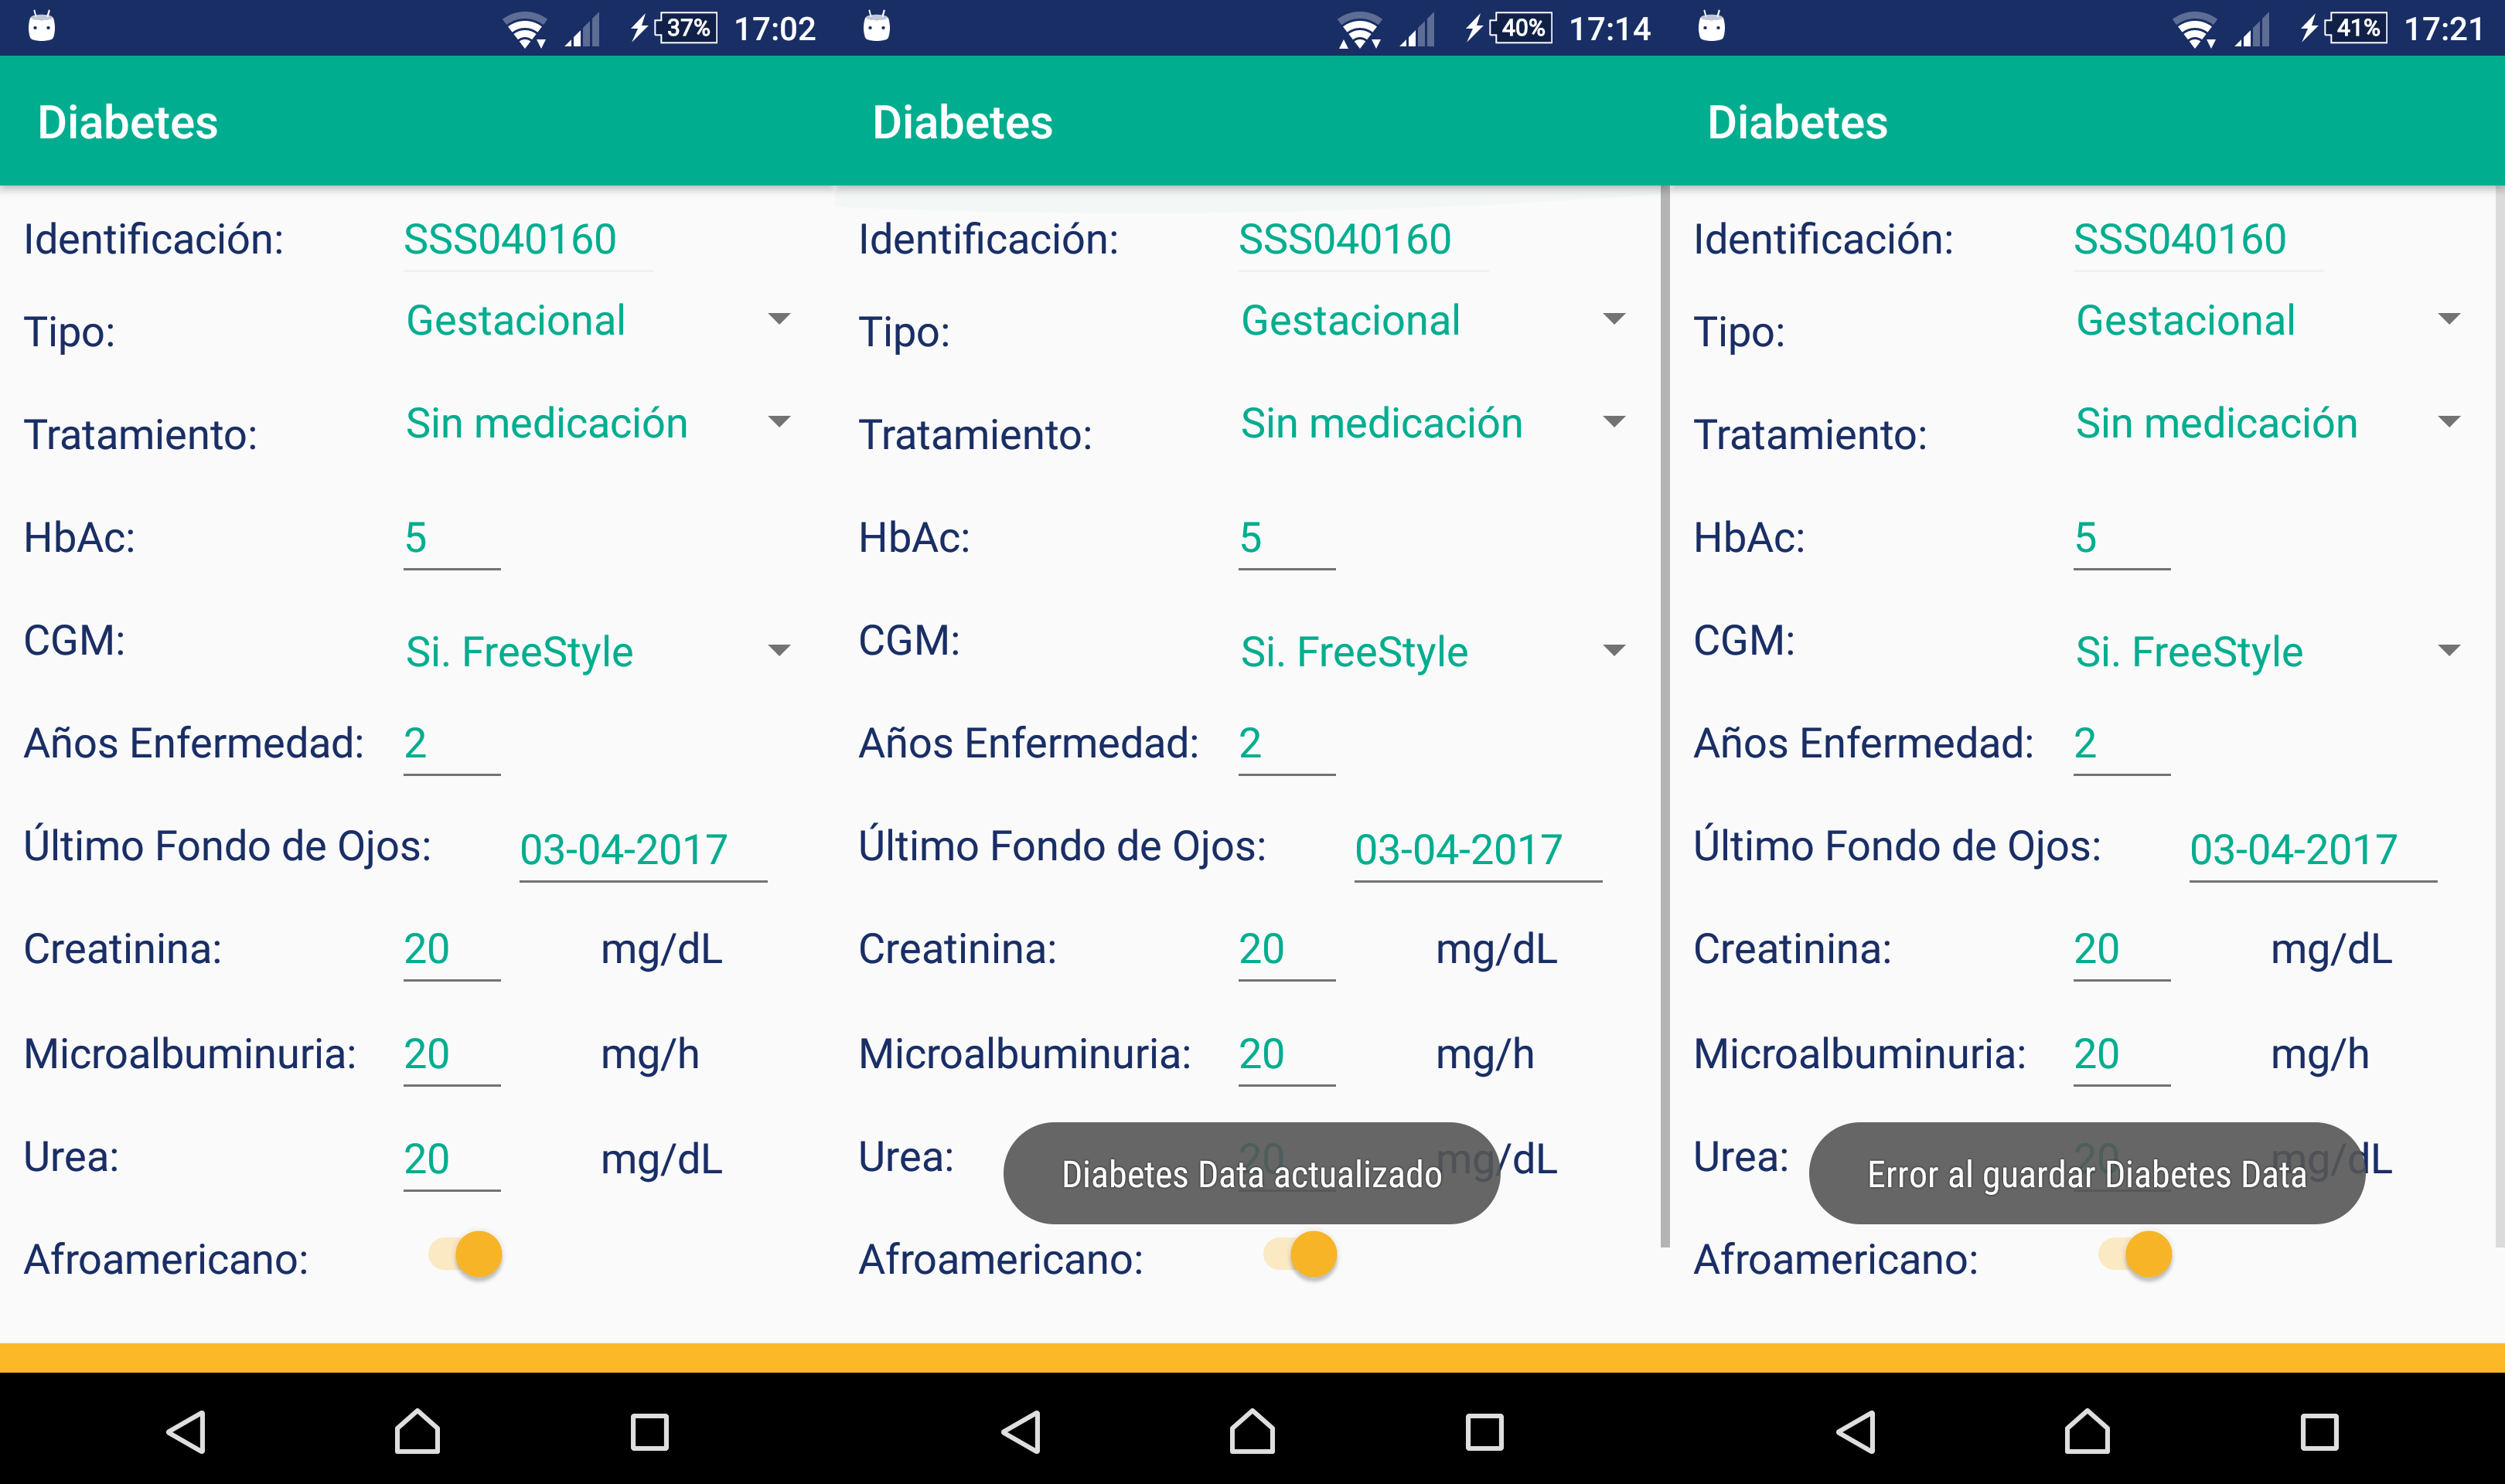
\includegraphics[height= 7cm]{capturas/diabetesFull.png}
\caption{Ventana - Diabetes}
\end{figure}

\begin{figure}[H]
\centering
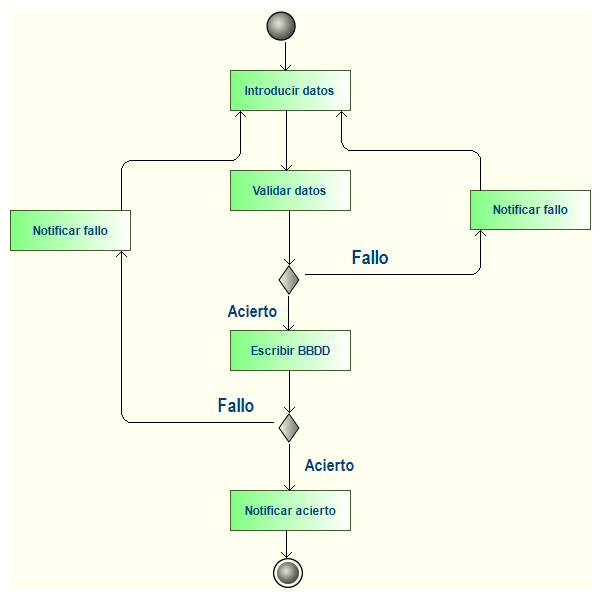
\includegraphics[height= 11cm]{diagramas/DiabetesActivitydiagram.png}
\caption{Diagrama de actividad - Diabetes}
\end{figure}

%COLESTEROL
\subsection {Calcular colesterol}

Deduce el valor de la lipoproteína de baja densidad (LDL) a partir de los valores introducidos por el usuario en los parámetros de entrada, a saber, lipoproteína de alta densidad (HDL), colesterol total y la cantidad de triglicéridos del paciente (Figura 2.39).
Tanto los parámetros de entrada como los resultados obtenidos se definen en mg/dl. (Figura 2.40)

\begin{figure}[H]
\centering
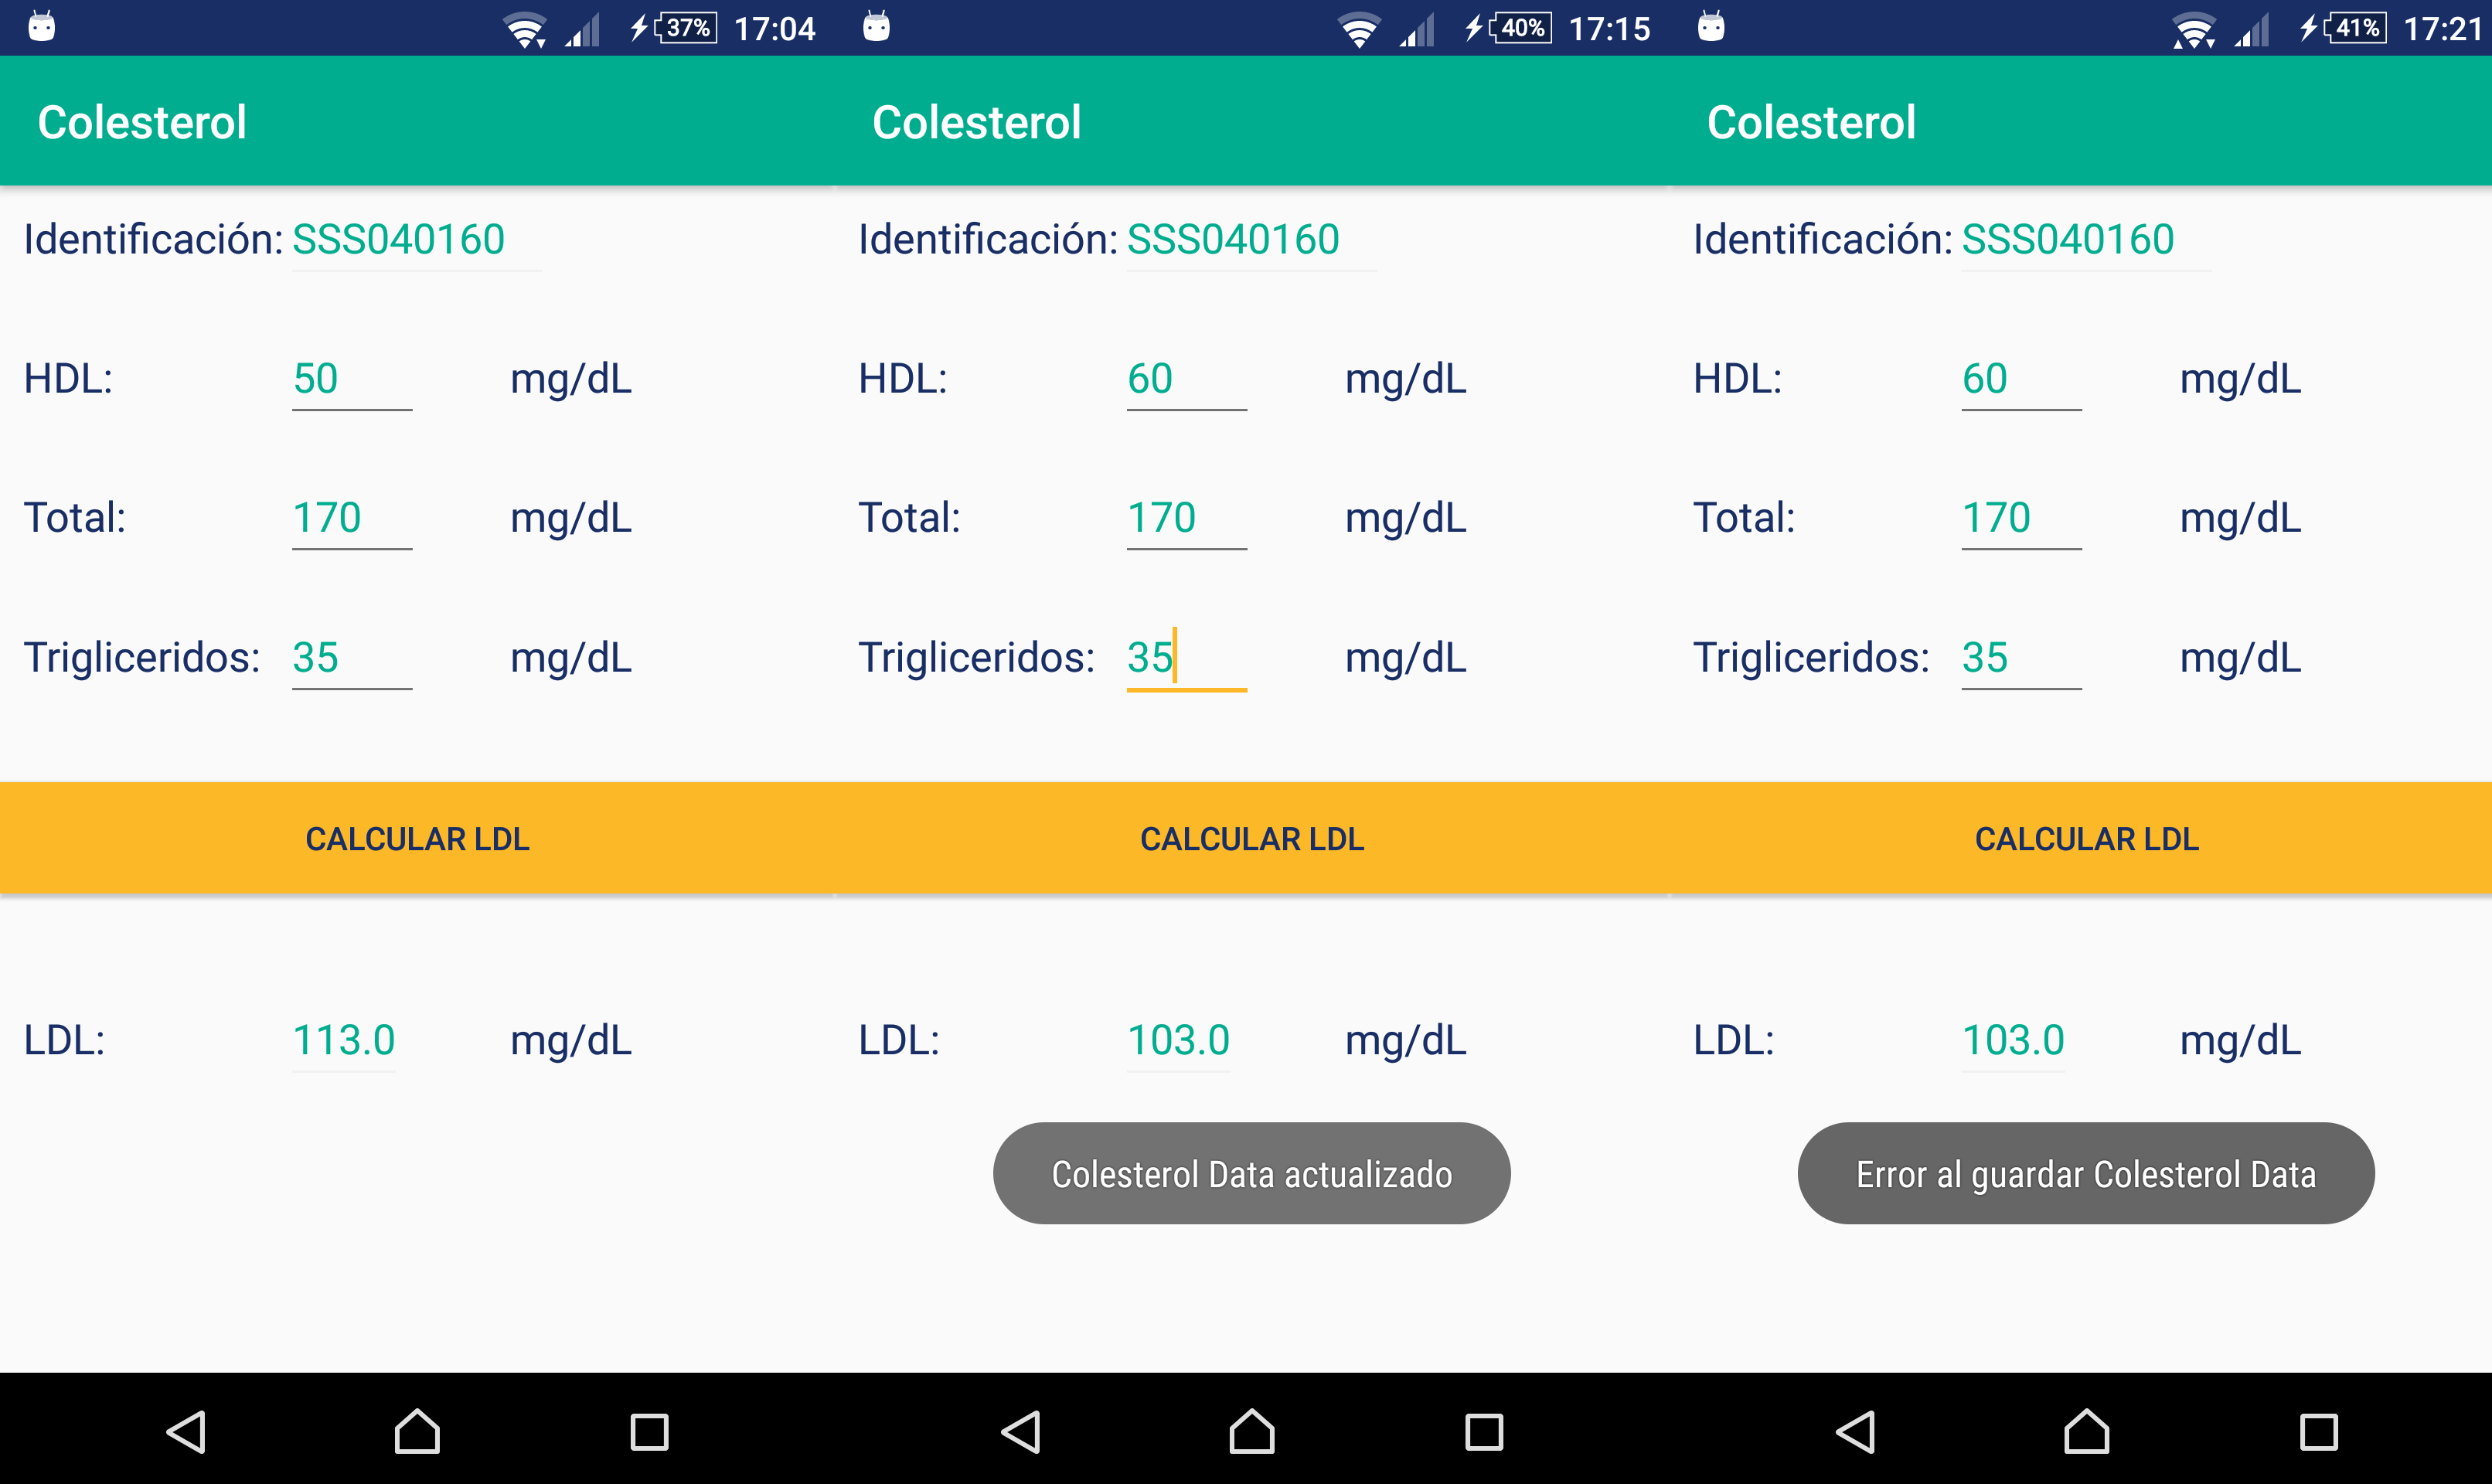
\includegraphics[height= 7cm]{capturas/colesterolFull.png}
\caption{Ventana - Colesterol}
\end{figure}

\begin{figure}[H]
\centering
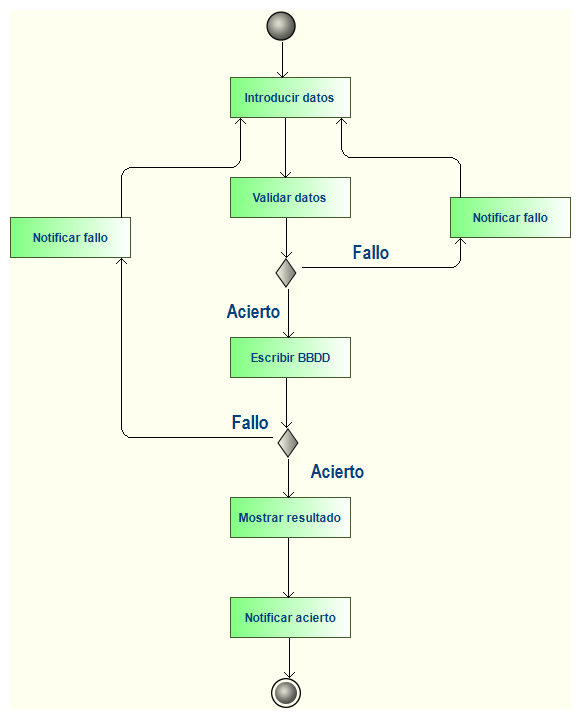
\includegraphics[height= 11cm]{diagramas/ColesterolpacienteActivitydiagram.png}
\caption{Diagrama de actividad - Colesterol}
\end{figure}

%HTA
\subsection {Calcular hipertensión arteria (HTA)}

Este término se refiere a la hipertensión arterial, es decir, el fenómeno que sucede si las paredes de las arterias están sometidas a una fuerza excesiva por la sangre que bombea el corazón al cuerpo del sujeto.
La aplicación solicita el valor que resulta del análisis de la presión arterial sistólica y diastólica (Figura 2.41). Los datos se expresan en mmHg. (Figura 2.42)

Las conclusiones de la aplicación son comunicadas mediante un mensaje claro que varía en función de la información suministrada.
Es notable mencionar que, en principio, los rangos de diastólica suelen tener una estrecha relación con los intervalos de valores relativos a la presión arterial sistólica. Sin embargo, la presión arterial sistólica tiene una mayor influencia que la distólica en la determinación del HTA. En consecuencia, si sucediese el caso en el que el valor de diastólica no entre en el conjunto de valores esperado la app decidirá el resultado en la forma habitual, pero mencionará dicha anomalía mediante un warning al médico.

\begin{figure}[H]
\centering
\includegraphics[height= 6.7cm]{capturas/HtaFull.png}
\caption{Ventana - Hipertensión Arterial}
\end{figure}

\newpage
\begin{figure}[H]
\centering
\includegraphics[height= 11cm]{diagramas/HtaActivitydiagram.png}
\caption{Diagrama de actividad - Hipertensión Arterial}
\end{figure}

\newpage
%IMC
\subsection {Calcular índice de masa corporal (IMC)}

De acuerdo con los estudios realizados, el IMC desempeña un rol significativo en los análisis del riesgo cardiovascular. Este índice establece una relación entre el peso y la altura y constituye un indicativo fiable para determinar casos de peso insuficiente, peso excesivo u obesidad en adultos (Figura 2.43). 
Atendiendo a la fórmula (\ref{eq:ej}):
\begin{equation}\label{eq:ej}
IMC = \frac{peso (kg)}{altura^2 (m)}
\end{equation}
El resultado se expresa en kg/m2. Asimismo, la aplicación interpreta el resultado obtenido y lo refleja en lenguaje cotidiano. (Figura 2.44)

\begin{figure}[H]
\centering
\includegraphics[height= 7cm]{capturas/ImcFull.png}
\caption{Ventana - Índice de Masa Corporal}
\end{figure}

\newpage
\begin{figure}[H]
\centering
\includegraphics[height= 11cm]{diagramas/ImcpacienteActivitydiagram.png}
\caption{Diagrama de actividad - Índice de Masa Corporal}
\end{figure}

\newpage
%TRATAMIENTO
\subsection {Tratamiento}

En función de los datos recogidos sobre el paciente, el médico tiene la posibilidad de dictar unas medidas para atender a las circunstancias del sujeto (Figura 2.45). Se dispone un resumen de la condición actual del paciente a partir de la cual el profesional pueda trabajar sin tener necesidad de consultar nuevamente los datos ofrecidos en otras pantallas. (Figura 2.46)

\begin{figure}[H]
\centering
\includegraphics[height= 7cm]{capturas/TratamientoFull.png}
\caption{Ventana - Tratamiento}
\end{figure}

\begin{figure}[H]
\centering
\includegraphics[height= 11cm]{diagramas/TrataminetoActivitydiagram.png}
\caption{Diagrama de actividad - Tratamiento}
\end{figure}

%DESCARGAR PDF
\subsection {Descargar PDF}

Es de notable conveniencia disponer de un método para almacenar y transmitir la documentación obtenida en esta aplicación. La capacidad de exportar estos datos en formato PDF habilita un sistema sencillo para compartir esta información con el paciente, personales relacionadas con el mismo u otros individuos cualificados...  Esta táctica favorece las acciones en el evento de que quieras imprimirlo, y archivarlo o clasificarlo, fomentando así la portabilidad (Figura 2.47). Además, este documento PDF permite compartir los resultados fácilmente mediante aplicaciones como Adobe Acrobat Reader, que posibilita el acceso a medios como el correo electrónico, Google Drive, etc. (Figura 2.48)

\begin{figure}[H]
\centering
\includegraphics[height= 7cm]{capturas/PDF_Full.png}
\caption{Ventana - Descargar PDF}
\end{figure}

\begin{figure}[H]
\centering
\includegraphics[height= 7cm]{diagramas/GenerarPDFActivitydiagram.png}
\caption{Diagrama de actividad - Descargar PDF}
\end{figure}

\newpage
%CERRAR SESION
\subsection {Cerrar sesión}

Da por concluida la actividad con su cuenta en la app, después de solicitar confirmación (Figura 2.49). (Figura 2.50)

\begin{figure}[H]
\centering
\includegraphics[height= 7cm]{capturas/log_out.png}
\caption{Ventana - Cerrar Sesión}
\end{figure}

\begin{figure}[H]
\centering
\includegraphics[height= 11cm]{diagramas/LogoutActivitydiagram.png}
\caption{Diagrama de actividad -  Cerrar Sesión}
\end{figure}


%%%%%%%%%%%%%%%%%%%%%%%%%%%%%%%%%%%%%%%%%%%%%%%%%%%%%%%%%%%%%%%%%%%%%%%%%%%%%%%%%%%%%%%%%%%%%%%%%%%%%%%%%%%%%%%%%%%%%%%%%
%																	ARQUITECTURA DE LA APLICACIÓN     																		             %
%%%%%%%%%%%%%%%%%%%%%%%%%%%%%%%%%%%%%%%%%%%%%%%%%%%%%%%%%%%%%%%%%%%%%%%%%%%%%%%%%%%%%%%%%%%%%%%%%%%%%%%%%%%%%%%%%%%%%%%%%
\chapter{Arquitectura de la aplicaci\'on}

El sistema consta de una aplicación Android que desempeña las funciones de cliente y de un servidor remoto que regula el acceso a la base de datos donde se almacenan los datos que precisa la app. Cada uno de los elementos involucrados en esta estructura serán explicados en los puntos desarrollados a continuación.

La ilustración, Figura 3.1, refleja un esquema de las tecnologías empleadas en la arquitectura del proyecto.

\begin{figure}[H]
\centering
\includegraphics[height= 11cm]{arquitectura.jpg}
\caption{Arquitectura de la aplicación}
\end{figure}

\newpage
%ANDROID STUDIO
\section {Aplicación Android}

La aplicación está dirigida a dispositivos Android. Está diseñada para garantizar la compatibilidad con versiones de Android API 21: 5.0 (Lollipop) o superiores, pero para obtener los óptimos resultados se recomienda el empleo de la versión de Android API 24: Android 7.0 (Nougat). 

De acuerdo con los datos suministrados por las fuentes [19] y [20] de la bibliografía, las versiones anteriores a Lollipop han experimentado un drástico decremento en su utilización cayendo a cifras en torno al 30\%. Por el contrario, los objetivos finales de nuestra aplicación cada vez poseen una mayor presencia en el mercado alcanzando a mayo de 2017 más del 70\% de los usuarios. Ello significa la garantía de que un gran número de los dispositivos Android existentes sean capaces de valerse de todas las funcionalidades ofrecidas por nuestra app.

En las siguientes figuras se evidencia la evolución de las versiones con más popularidad en el año que va de 2016 al presente 2017.

\begin{figure}[H]
\centering
\includegraphics[height= 6.5cm]{android_2016_tabla.png}
\caption{Gráfico de versiones Android en el mercado en 2016}
\end{figure}

En 2016 ya se advertía un refuerzo en la posición de Lollipop incrementando en un 2\%  sus seguidores en únicamente un mes, al mismo tiempo que se producía una caída de las cifras de versiones anteriores en el mismo periodo de tiempo. La situación de KitKat sufría el infortunio de verse deteriorada en un 1.2\%, Jelly Bean bajó 2.4\% y versiones todavía más arcaicas se ven en proceso de desaparición.

\newpage
\begin{figure}[H]
\centering
\includegraphics[height= 8cm]{android_2017_tabla.png}
\caption{Gráfico de versiones Android en el mercado en 2017}
\end{figure}

En 2017 esta tendencia negativa en las versiones antiguas se confirmó. En este año la popularidad de KitKat se reduce de 34.3\% a la baja cantidad de 18.8\% y las versiones anteriores entran en el límite de su vida siendo incapaces de alcanzar la dimensión de dos cifras. Las circunstancias son muy diferentes para las versiones a las que esta aplicación va dirigido. En el análisis de 2016 Lollilop se erigía como el gigante entre sus competidores estando la nueva versión Marshmallow en sus inicios con 2.3\%. Sin embargo, en 2017 Lollipop mantiene su puesto en la vanguardia con un 32\% pero Marshmallow amenaza con sobrepasarle con un 31.2\%. Además, la última versión de Android bajo el nombre de Android Nougat y objetivo ideal de nuestra app experimenta un repunte de abril a mayo pasando del 4.9\% al 7.1\%. Su futuro parece prometedor como consecuencia de las nuevas actualizaciones y la nueva generación de dispositivos que llegan al mercado con esta versión de fábrica, como el LG G6	 o el Samsung Galaxy S8.

En definitiva, basándonos en los datos podemos esperar la eliminación inminente de las versiones no soportadas y el auge inmediato de Android Nougat en los próximos meses, asegurando el futuro de nuestra aplicación.

La aplicación cliente desarrollada con este IDE constituye nuestra principal y única fuente de datos, a través de la cual el médico puede tener en todo momento al alcance de su mano los datos de un paciente si necesitase consultar o actualizar la información del mismo. La aplicación móvil tiene como finalidad principal la determinación del índice de riesgo cardiovascular a partir de la facilitación de los datos médicos analizados sobre un conjunto de parámetros de influencia (imc, tensión arterial, colesterol...).

\newpage
%BASE DE DATOS
\section {Base de datos}

La base de datos está alojada en una máquina virtual en un servidor y satisfacerá las funciones relativas al almacenaje de la información generada por la aplicación. 

En nuestra aplicación se requiere la lectura, escritura y manipulación de los datos facilitados por el cliente. Estos registrarán información relativa a los médicos y pacientes tales como los datos personales de los mismos, el estado médico del paciente...

Como consecuencia del requerimiento de estar en capacidad de realizar modificaciones a los datos almacenados, y no solamente lecturas y escrituras, descartamos el empleo de bases de datos no relacionales. Los datos presentarán una organización estructurada, identificados unívocamente valiéndose de una clave primaria. En concreto, por razones expuestas posteriormente en Modelo de datos nos decantamos por la utilización de MySQL.

%SERVIDOR
\section {Servidor}

Para hacer las funciones de servidor empleamos una máquina virtual con el Sistema Operativo Linux alojada en un ordenador remoto. Este servidor dispondrá del acceso a la base de datos y otras herramientas necesarias para el correcto manejo de la misma.


%%%%%%%%%%%%%%%%%%%%%%%%%%%%%%%%%%%%%%%%%%%%%%%%%%%%%%%%%%%%%%%%%%%%%%%%%%%%%%%%%%%%%%%%%%%%%%%%%%%%%%%%%%%%%%%%%%%%%%%%%
%																		MODELO DE DATOS    																		                       %
%%%%%%%%%%%%%%%%%%%%%%%%%%%%%%%%%%%%%%%%%%%%%%%%%%%%%%%%%%%%%%%%%%%%%%%%%%%%%%%%%%%%%%%%%%%%%%%%%%%%%%%%%%%%%%%%%%%%%%%%%
\chapter{Modelo de datos}

En nuestra aplicación móvil es de vital importancia el tratamiento de una gran cantidad de datos, ya que estos son lo base para llevar acabo los fines de nuestra aplicación. En un estudio inicial concluimos que en nuestra aplicación se distinguían dos grupos principales, pacientes y médicos. 

Se utilizó MySQL para abordar este problema, puesto que es perfecta tanto para el desecho de información como para las búsquedas específicas y actualizaciones de datos.

Describimos en detalle las principales características del modelo de datos.

Nuestro enfoque es apoyarnos en el diagrama entidad-relación en conjunción con el relacional para su diseño. Tras terminar el proceso anterior, usamos la herramienta MySQL Workbench para obtener un diagrama que permita presentar los contenidos con un perfil visual atractivo.

\newpage
%\begin{landscape}
	\begin{figure}[H]
	\centering
	\includegraphics[height= 16cm]{bd_model.png}
	\caption{Base de datos relacional}
	\end{figure}
%\end{landscape}
\newpage

Contamos con 10 tablas relacionadas entre sí mediante claves foráneas y atributos por medio de una estructura clara y eficiente.

\noindent
\textbf {medico\_validar}

Engloba la información relativa a los aspirantes a médico en nuestra aplicación. Estos datos son los que permitirán al administrador decidir si validar a la persona asociada como profesional sanitario.
\begin{itemize}
	\item id: clave primaria autoincremental.
	\item nombre: guarda el nombre del aspirante.
	\item apellidos: guarda los apellidos del solicitante.
	\item telefono: contiene el teléfono del aspirante.
	\item password: almacena la contraseña del aspirante.
	\item colegiado: guarda el número del colegiado (9 dígitos) del solicitante.
	\item mail: contiene el correo del candidato.
\end{itemize}

\noindent
\textbf {medico}

Especifica los datos personales del médico.
\begin{itemize}	
	\item nombre: contiene el nombre del médico.
	\item apellidos: guarda los apellidos del médico.
	\item telefono: almacena el teléfono del médico.
	\item password: contiene la contraseña del médico.
	\item colegiado: almacena el número del colegiado (9 dígitos) del médico. Es la clave primária porque debe definir unívocamente al profesional.
	\item mail: guarda el correo del médico.
\end{itemize}

\noindent
\textbf {medico\_roles}

Diferencia entre los distintos niveles de permisos concedidos a cada usuario.
\begin{itemize}
	\item id: clave primaria autoincremental.
	\item colegiado: referencia al identificador único del médico.
	\item rol: define si el profesional tiene privilegios administrativos (0) o no (1).
\end{itemize}

\noindent
\textbf {medico\_paciente}

Relaciona cada paciente con su(s) médico(s) asociado(s).
\begin{itemize}
	\item id: clave primaria autoincremental.
	\item colegiado: referencia al identificador único del médico.
	\item paciente\_id: referencia al identificador único del paciente.
\end{itemize}

\noindent
\textbf {pacientes}

Especifica los datos más importantes de cada paciente.
\begin{itemize}
	\item paciente\_id: clave primaria que define al paciente. Consiste en las tres iniciales de nombre y apellidos seguido de la fecha de nacimiento formato ddmmyy.
	\item sexo: establece el género del paciente. M (Masculino), F (Femenino).
	\item edad: guarda la edad del paciente.
	\item regicor: índice de riesgo cardiovascular expresado en tanto por ciento.
	\item finalTratamiento: almacena la información relativa al tratamiento específico designado por el médico para las circunstancias del paciente.
\end{itemize}

\noindent
\textbf {tabaquismo}

Relaciona cada paciente con su registro de tabaquismo.
\begin{itemize}
	\item pacienteId: referencia al identificador único del paciente.
	\item cantidad: cigarrillos consumidos por el paciente en un día.
	\item adiccion: designa los años de vicio del paciente.
	\item ipa: archiva el índice de paquetes al año.
\end{itemize}

\noindent
\textbf {imc}

Vincula cada paciente con la información relativa al imc.
\begin{itemize}
	\item pacienteId: referencia al identificador único del paciente.
	\item altura: contiene la estatura en metros del paciente.
	\item peso: almacena el peso en kilogramos del paciente.
	\item imc: guarda el ínidce de masa corporal.
\end{itemize}

\noindent
\textbf {hta}

Establece una conexión entre el paciente y los datos de hipertensión arterial.
\begin{itemize}
	\item pacienteId: referencia al identificador único del paciente.
	\item sistolica: almacena la presión arterial sistólica del paciente (mmHg).
	\item distolica: contiene la presión arterial diastólica del paciente (mmHg).
\end{itemize}

\noindent
\textbf {colesterol}

Relaciona cada paciente con sus valores de colesterol.
\begin{itemize}
	\item pacienteId: referencia al identificador único del paciente. 
	\item total: almacena la cantidad de colesterol total del paciente (mg/dl).
	\item hdl: contiene la cantidad de colesterol bueno del paciente (mm/dl).
	\item trigliceridos: almacena el nivel de trigliceridos en sangre del paciente (mm/dl).
	\item ldl: guarda la cantidad de colesterol malo del paciente (mm/dl).
\end{itemize}

\noindent
\textbf {diabetes}

Enlaza cada paciente con la información concerniente a su estado de diabetes.
\begin{itemize}
	\item pacienteId: referencia al identificador único del paciente. 
	\item tipo: designa el tipo de diabetes del paciente.
	\item tratamiento: procedimiento asignado al paciente. Por ejemplo Gestacional.
	\item hbac: almacena el nivel de hemoglobina glicosilada en sangre.
	\item monitorizacion: monitor continuo de glucosa.
	\item yearEnfermo: índica el número de años de enfermedad del paciente.
	\item lastEyes: fecha de último fondo de ojos.
	\item creatinina: guarda la cantidad de creatinina (mg/dl).
	\item microalbuminuria: define el nivel de excreción de albúmina por la orina (md/h).
	\item raza: determina si el paciente es afroamericano (Yes) o no (No).
	\item urea: guarda el nivel de urea (principal producto de degradación del metabolismo de las proteínas) en sangre expresado en mg/dl.
	\item fecha: momento en el que se introdujeron dichos datos.	
\end{itemize}


%%%%%%%%%%%%%%%%%%%%%%%%%%%%%%%%%%%%%%%%%%%%%%%%%%%%%%%%%%%%%%%%%%%%%%%%%%%%%%%%%%%%%%%%%%%%%%%%%%%%%%%%%%%%%%%%%%%%%%%%%
%																		     TECNOLOGIAS  																		                                  %
%%%%%%%%%%%%%%%%%%%%%%%%%%%%%%%%%%%%%%%%%%%%%%%%%%%%%%%%%%%%%%%%%%%%%%%%%%%%%%%%%%%%%%%%%%%%%%%%%%%%%%%%%%%%%%%%%%%%%%%%%
\chapter{Tecnolog\'ias}

Presentamos a continuación las tecnologías empleadas para cada módulo del proyecto. 

%ANDROID STUDIO
\section {Aplicación Android}

Usamos fundamentalmente Java y el SDK de Android. Debido al rápido proceso de familiaridad y el amplio número de funcionalidades para el desarrollo y codificación, usaremos Android Studio como el IDE seleccionado. Su amplia comunidad y soporte suponen un poderoso apoyo a los desarrolladores, proporcionando una curva de evolución estable y fácilmente adaptable a las últimas tecnologías.

Enfocamos el diseño de la interfaz utilizando las herramientas ofrecidas por la plataforma de Android basadas en XML. Suministra una interfaz gráfica, la cual te permite reducir el tiempo de diseño enormenente al generar el código automáticamente. El funcionamiento básico consiste en el establecimiento de layouts, entradas de texto, labels, botones... en una pantalla virtual (vista previa) escogidos de entre una colección de los mismos. 

%BASE DE DATOS
\section {Base de datos}

Para la manipulación de los datos que precise nuestra aplicación, nos valdremos de MySQL por las razones expuestas a continuación:

\begin{enumerate}
	\item Su naturaleza de código abierto, la cual favorece su mantenimiento y limita nuestra dependencia en entidades particulares.

	\item El soporte proporcionado para su migración a distintos sistemas operativos garantizando de esa forma la portabilidad.

	\item Su carácter idóneo para el acceso de bases de datos en Internet como resultado de su alta conectividad, velocidad y seguridad.

	\item Su bajo costo en requerimientos para la elaboración de base de datos, el cual resulta en que se pueda ejecutar en una máquina con escasos recursos sin impedimentos. Esta propiedad es de especial importancia en nuestro caso, ya que estamos confinados a una máquina virtual con bajas especificaciones para  desempeñar las funciones de servidor (más información sobre esta máquina en el punto Servidor y unidad de procesamiento de esta mismo capítulo).
\end{enumerate}

% PHP
\section {PHP}

Para afrontar el establecimiento de la comunicación entre la base de datos y la aplicación cliente de Android empleamos el lenguaje PHP.

Nuestras bases para esta decisión son nuestro alto grado de familiaridad con el mismo, su fácil acceso a la información almacenada en la base de datos y su impulso a la seguridad al ejecutarse en el lado del servidor siendo invisible al cliente. Adicionalmente, dispone de una comunidad activa colosal avalando la capacidad de asesoramiento en caso de tener cualquier duda relativa al desarrollo o protección del código.

%GIT
\section {GitHub}

Con el fin de gestionar las distintas versiones nos serviremos de GitHub, ya que ofrece numerosas opciones a los estudiantes para un cómodo control de la evolución del proyecto. De esta forma, la evolución del proyecto queda registrada proporcionándonos la posibilidad de revertir modificaciones erróneas al mismo tiempo que notifica a nuestro tutor asignado u otros interesados de la progresión de la actividad. 

A todo lo mencionado anteriormente hay que añadir que su enorme popularidad entre la comunidad de código abierto favorece la visibilidad de nuestro trabajo. Esto incentiva la cooperación con nuestros directores a la vez que se fomenta la búsqueda de potenciales seguidores, los cuales podrían proponer mejoras o correciones al diseño.

\noindent Puedes consultar los detalles de nuestra app en: \url{https://github.com/tfgcardiovascular}

%SERVIDOR Y UNIDAD DE PROCESAMIENTO
\section {Servidor y unidad de porcesamiento}

Para la cuestión del servidor, hemos diseñado una máquina virtual linux para desempeñar este cometido. La máquina virtual empleará las facilidades ofrecidas por Apache Tomcat para la gestión de la comunicación entre el servidor y la aplicación móvil de android que actúa como el cliente.

%Hablar de Tomcat y de la maquina virtual. modo de comunicacion...


%%%%%%%%%%%%%%%%%%%%%%%%%%%%%%%%%%%%%%%%%%%%%%%%%%%%%%%%%%%%%%%%%%%%%%%%%%%%%%%%%%%%%%%%%%%%%%%%%%%%%%%%%%%%%%%%%%%%%%%%%
%																		    	 CONCLUSIONES														                             			             %
%%%%%%%%%%%%%%%%%%%%%%%%%%%%%%%%%%%%%%%%%%%%%%%%%%%%%%%%%%%%%%%%%%%%%%%%%%%%%%%%%%%%%%%%%%%%%%%%%%%%%%%%%%%%%%%%%%%%%%%%%
\chapter{Conclusiones}

La a meta a alcanzar con el desarrollo de este Trabajo de Fin Grado es explorar los límites de la coexistencia entre las herramientas informáticas y el desempeño de la actividad sanitaria. La creciente participación de las ramas de la computación en diversos sectores de la industria, servicios y ocio, exige que se mantengan a la vanguardia de las últimas tecnologías.

En este aspecto, la medicina se ha sucedido una evolución lenta en lo que se refiere a esta revolución hacia la automatización de los procesos. Por todo ello, el presente proyecto toma como objetivo la innovación en este campo.

Tras acabar el TFG y registrar el progreso en la presente memoria, es la perfecta ocasión para realizar un análisis de los ideales alcanzados.

Con la creación de esta aplicación móvil hemos experimentado el avance continuo de las plataformas tecnológicas. En este año Android Studio se ha beneficiado de sucesivas actualizaciones que le han permitido adaptarse a los últimos requisitos y mejorar la interacción de los desarrolladores. La introducción del nuevo botón de lanzamiento del emulador de Android, el cual permite implementar cambios rápidos sin tener que cargar de nuevo el sistema, ha significado una excelente novedad para nosotros ya que es frecuenta las constantes comprobaciones de pequeñas modificaciones. No obstante, este acontecimiento también exhibe implicaciones que requieren un esfuerzo adicional por parte de los programadores. La aparición de una nueva versión suele resultar en numerosos casos de funciones obsoletas, presionando a su adecuación a la nueva versión si se desea evitar posibles resultados no previstos.

Aunque hemos vivido complicaciones en nuestro trabajo con este IDE, especialmente en la puesta en marcha del TFG, nuestra experiencia nos ha permitido adquirir nuevos conocimientos de utilidad y los resultados han sido gratificantes. 

En el plano de lo que puede llegar a contribuir a la sociedad, es destacable la colaboración entre los médicos para tratar a un mismo paciente. Es habitual que las aplicaciones de esta naturaleza tengan un enfoque en el lado del paciente, desempeñando un servicio centrado en calcular los resultados (imc, hta, ipa, riesgo cardiovascular...). Por el contrario, en adicción a estas operaciones, ofrecemos un sistema de gestión de los pacientes asistiendo a los médicos.

Teniendo en cuenta lo establecido, podemos alegar que nuestros propósitos han sido hechos realidad al implementar una app que cubra una necesidad a las que la competencia no ha dedicado una especial atención.
%\MakeUppercase{Enfermedades Cardiovasculares}
En definitiva, estimamos que el desarrollo de esta aplicación móvil nos ha proporcionado una visión más madura sobre los inconvenientes que sobrevienen al tratar con un proyecto orientado al público y los requerimientos que conlleva la producción de un trabajo de larga duración, como el acondicionamiento a la actualización de las tecnologías empleadas.


%%%%%%%%%%%%%%%%%%%%%%%%%%%%%%%%%%%%%%%%%%%%%%%%%%%%%%%%%%%%%%%%%%%%%%%%%%%%%%%%%%%%%%%%%%%%%%%%%%%%%%%%%%%%%%%%%%%%%%%%%
%																		    	 CONCLUSIONS														                             			             %
%%%%%%%%%%%%%%%%%%%%%%%%%%%%%%%%%%%%%%%%%%%%%%%%%%%%%%%%%%%%%%%%%%%%%%%%%%%%%%%%%%%%%%%%%%%%%%%%%%%%%%%%%%%%%%%%%%%%%%%%%
\addtocounter{chapter}{-1}
\selectlanguage{english}
\chapter{Conclusions}

The goal to be achieved with the development of this Final Degree Work is to explore the limits of the coexistence between computer tools and the performance of health activity. The increasing participation of the branches of the computer in diverse sectors of the industry, services and leisure, demands that they remain at the forefront of the latest technologies.

In this respect, medicine has undergone a slow evolution in regard to this revolution towards the automation of processes. For all this, the present project aims at innovation in this field.

After finishing the TFG and recording the progress in the present report, it is the perfect occasion to carry out an analysis of the ideals reached.

With the creation of this mobile application we have experienced the continuous advancement of technology platforms. This year Android Studio has benefited from successive updates that have allowed it to adapt to the latest requirements and improve the interaction of developers. The introduction of the new launch button of the Android emulator, which allows you to implement quick changes without having to reload the system, has meant an excellent novelty for us as it is frequent constant checks for minor modifications. However, this event also has implications that require additional effort on the part of programmers. The appearance of a new version usually results in numerous cases of obsolete functions, pressing its adaptation to the new version if it is desired to avoid possible unforeseen results.

Although we have experienced complications in our work with this IDE, especially in the implementation of the TFG, our experience has allowed us to acquire new knowledge of usefulness and the results have been rewarding.

In terms of what can contribute to society, it is remarkable the collaboration between doctors to treat the same patient. It is common for applications of this nature to have a patient-centered approach, performing a service centered on calculating the results (bmi, hta, ipa, cardiovascular risk ...). On the contrary, in addiction to these operations, we offer a management system for patients attending physicians.

Given the established, we can claim that our purposes have been realized when implementing an application that meets a need that the competition has not dedicated a special attention.

In short, we believe that the development of \MakeUppercase {Cardiovascular Diseases} has given us a more mature view of the drawbacks of dealing with a public-oriented project and the requirements of producing a long-term work, such as Conditioning to the updating of the technologies used.


%%%%%%%%%%%%%%%%%%%%%%%%%%%%%%%%%%%%%%%%%%%%%%%%%%%%%%%%%%%%%%%%%%%%%%%%%%%%%%%%%%%%%%%%%%%%%%%%%%%%%%%%%%%%%%%%%%%%%%%%%
%																		     TRABAJO FUTURO  														                                  			   %
%%%%%%%%%%%%%%%%%%%%%%%%%%%%%%%%%%%%%%%%%%%%%%%%%%%%%%%%%%%%%%%%%%%%%%%%%%%%%%%%%%%%%%%%%%%%%%%%%%%%%%%%%%%%%%%%%%%%%%%%%
\selectlanguage{spanish}
\chapter{Trabajo futuro}
%\MakeUppercase{Enfermedades Cardiovasculares}
El análisis realizado en el capítulo anterior nos proporciona una buena base para deducir potenciales mejoras en la aplicación:

\begin{enumerate}
	\item \textbf {Extender el servicio a otros sistemas operativos (SO).}

Uno de los aspectos más importantes a tener en cuenta en aplicaciones de esta índole es restringir lo mínimo posible el público al que está dirigido. En consiguiente, estamos estudiando una metodología para mejorar la portabilidad de esta aplicación. Entre nuestras investigaciones, cabe destacar la existencia de Xamarin que permite llevar la app a Windows Phone, iOS y Android a través de un mismo IDE. Sin embargo, está fundamentado en el uso de código programado en C\# y ello supone la traducción de la codificación actual en una entendible por Xamarin.

	\item \textbf {Sistema de notificaciones.} 
%\MakeUppercase{Enfermedades Cardiovasculares}
En la app es preciso que el administrador valide tus datos de registro para la activación de tu cuenta. Desafortunadamente, en la fecha presente el médico no es informado de la confirmación o el rechazo de su solicitud, siendo este un inconveniente si esta app se lanzase al mercado. La solución planteada consiste en mensaje automático de notificación personalizado informándote de la decisión sobre tu petición. Manteniendo esta idea en mente, la aplicación solicita tu dirección de correo electrónico en el registro. 

Otra de las situaciones en las que sería aconsejable disponer de una notificación es al compartir un paciente con otros médicos. Los afectados recibirían noticia esta situación en forma de pop-up al acceder a su lista de pacientes.

	\item \textbf {Historial.}

Es frecuente que los diagnósticos presentes se vean influenciados por los acontecidos en el pasado. Para resolver este dilema, se expandirá la funcionalidad de la aplicación mediante la inclusión de un registro de los diferentes resultados identificados por su fecha de creación. Con el fin de reflejar en una única imagen la esencia de esta información, planeamos generar una gráfica a partir de estos datos permitiendo así al profesional adquirir una compresión rápida de la evolución de forma sencilla.

	\item \textbf {Diversidad lingüística.}

De acuerdo con la premisa de expansión de usuarios de la mejora inicial, es oportuno la comunicación de los datos en diversos lenguajes. Con la afluencia actual y posiblemente creciente de refugiados, la incorporación de esta nueva funcionalidad facilitará la labor del personal sanitario logrando de esta forma favorecer la ampliación de fronteras. Actualmente la app sólo dispone de lenguaje castellano, por lo que el proceso de traducción será bastante costoso si se marca como objetivo una interpretación fiel al significado original de las palabras y frases utilizadas, al requerirse personal con conocimiento adecuados para solventar esta dificultad.

	\item \textbf {Interpretar los datos suministrados por Monitores Continuos de Glucosa (GCM).}

En la actualidad existen sistemas GCM que te permiten obtener información sobre tus niveles de glucosa en todo momento. La meta considerada es establecer una comunicación entre nuestra app y estos dispositivos (Dexcom, FreeStyle...) facilitando así los datos de entrada de forma fiable sin necesidad de proporcionarlos manualmente.

	\item \textbf {Hacer uso de la cámara para determinar el HTA.} 

Siguiendo el principio del caso anterior, se añadirá un método para medir las cantidades representantes de la tensión arterial. Tomando como referencia aplicaciones existentes en el mercado que implementan esta funcionalidad, hemos determinado el uso de la cámara como la herramienta más apropiada para la obtención de los datos debido a estar presente en básicamente la totalidad de los dispositivos móviles. Su funcionamiento se basa en detectar los leves cambios de color del dedo causados por sus capilares sanguíneos, que se expanden y se contraen con cada latido del corazón. Esto permite que la aplicación medir el pulso.

	\item \textbf {Aplicación web para el ordenador.}
%\MakeUppercase{Enfermedades Cardiovasculares}
Con el fin de evitar que la aplicación sea inaccesible para los métodos convencionales hemos decidido ampliar el servicio con un futuro servicio web. Esto permite la libertad de movimiento propia de las aplicaciones móviles, al mismo tiempo que se garantiza la posibilidad de valerse de herramientas exclusivas de ordenadores para complementar la información de la aplicación.
\end{enumerate}


%%%%%%%%%%%%%%%%%%%%%%%%%%%%%%%%%%%%%%%%%%%%%%%%%%%%%%%%%%%%%%%%%%%%%%%%%%%%%%%%%%%%%%%%%%%%%%%%%%%%%%%%%%%%%%%%%%%%%%%%%
%																		          DIVISIÓN DEL TRABAJO            												                                                                  %
%%%%%%%%%%%%%%%%%%%%%%%%%%%%%%%%%%%%%%%%%%%%%%%%%%%%%%%%%%%%%%%%%%%%%%%%%%%%%%%%%%%%%%%%%%%%%%%%%%%%%%%%%%%%%%%%%%%%%%%%%
\chapter{División del trabajo}

%RICARDO
\section{Ricardo Cajigas Arenas}
Para el desarrollo de este trabajo fue necesario la completa colaboración entre todos los miembros del equipo. Ambos nos hemos esforzado en obtener el resultado más óptimo para los obstáculos que ha ido encontrando cualquiera de los dos.

Las tareas solicitadas por el proyecto fueron distribuidas en función de las especialidades de los integrantes, sin por ello desatender la posibilidad de auxiliar al compañero si este se viese en un dilema.

Especificamente, mi colaboración a este proyecto ha hecho enfásis en el diseño del esquema organizativo de la app y la implementación gráfica de las interfaces. Asi como ayudar en la codificación a mi compañero en situaciones donde había un alta carga de trabajo en esta parte.

Como consecuencia de la necesidad de Android Studio para este proyecto, dediqué un tiempo inicial a formarme en el manejo de este IDE. Una pequeña parte del esfuerzo destinado a este fin queda reflejado en la información expuesta en la bibliografía.

En los comienzos centré mis esfuerzos en la creación de bocetos que sirviesen de orientación para el desarrollo de la versión final. Con la ayuda de los colaboradores escogimos a partir de los croquis mencionados los elementos a añadir, modificar y/o eliminar y la organización de las ventanas que considerabamos más adecuada para la finalidad de esta aplicación.

Una vez concluida la preparación anterior, tras terminar el diseño de una primera versión de la ventana de login procedimos en equipo a establecer la comunicación entre la misma y la base de datos.
Tras la redacción del código por parte de mi compañero encontramos nuestro primer obstáculo. La desorganización en la información y documentación disponible en Internet resultó en equivocaciones en las suposiciones iniciales sobre la metodología requerida para establecer la conexión.
Una vez superado este impedimento, comenzamos la elaboración de las tareas relativas al registro. El proceso fue relativamente sencillo y no se sucedieron complicaciones adicionales que retrasasen la finalización de este punto.

En este momento, tomamos conciencia de la necesidad de garantizar la legitimidad de los usuarios registrados. En una reunión con nuestro tutor concluimos la conveniencia de introducir un nuevo rol de administrador que confirmase los registros verídicos. 

Este nuevo papel supuso un replanteamiento de la estructura de la aplicación. Mientras mi compañero completaba la lógica para otras secciones, inicié el análisis de las interfaces necesarias y los elementos a añadir.

Tras sucesivas reuniones con el tutor y feedbacks suministrados por Rafa, delimitamos una imagen general de la apariencia que tomaría nuestra aplicación en su versión final. Sólo fueron necesarias algunas modificaciones para mejorar eficientemente lo que es hoy día esta aplicación móvil.

En los sucesivos meses, contribuí en la implementación del código aportando sugerencias y buscando información requerida para la mejora de la funcionalidad tratada actualmente.
Asimismo, realizé las modificaciones pertinentes al diseño de acuerdo al feedback proporcionado por los colaboradores y necesidades del otro miembro del equipo. Un ejemplo de estas ocurrencias es el abandono de la idea inicial en la que se planteó utilizar una base de datos propia que suministrase información de los fármacos al usuario. En su lugar, decidimos valernos de una base exterior ya que los costes de rendimiento serían demasiado grandes para un mínimo beneficio.

Mediante herramientas de diseño, Ricardo se ha encargado de gran parte de los trabajos de maquetación de los documentos, y de la estructuración e investigación de recursos para las obstrucciones que han ido apareciendo durante la evolución de este proyecto. También he colaborado con el otro miembro del equipo en la redacción de la presente memoria.

Las capturas de pantalla del móvil que sirven de ilustración complementaria en la especificación de las funcionalidades e itentan reflejar en la mayor medida de lo posbible todos los posibles situaciones en las que se podría encontrar el usuario, han sido realizadas por mí. También, he elaborado los diagramas de caso de uso, actividades... expuestos en la presente memoria.

Para finalizar, querría destacar que la organización ha sido eficiente y hemos procurado realizar los objetivos al máximo de nuestras facultades. Esta realidad ha sido posible solamente al tratarse de un proyecto que cuanto más trabajábamos en él más despertaba nuestra ilusión e interés. Sin la complicidad con Ángel hubiera sido imposible alcanzar un resultado tan positivo como es este TFG. 
 
%ANGEL
\newpage
\section{José Ángel Sánchez Martín}
Es mi deseo confirmar que solamente a través de la participación conjunta de ambos miembros del equipo, ha sido posible la finalización de un proyecto de esta envergadura.
Todas las partes involucradas han participado y asistido en el trabajo del resto de los integrantes del grupo, proporcionando nuevos puntos de vista que han enriquecido los frutos finales de la labor realizada.

Sin embargo, la existencia de diferencias en las capacidades de cada miembro es una conclusión inevitable. Ello significa que es más adecuado adjudicar determinados cometidos del proyecto a una persona específica.

En concreto, mi participación en esta aplicación ha estado más centrada en la implementación del código requerido por las distintas funcionalidades ofrecidas por la app.

En los primeros días me familiarizé con las funcionalidades ofrecidas por Android Studio y sus convencionalismos. Para ello, estudié tutoriales y consulté libros, poniendo finalmente los conocimientos adquiridos en práctica mediante la realización de casos introductorios ofrecidos en la red.

Finalizado un primer contacto con este nuevo IDE, mientras mi compañero delineaba la apariencia y elementos interactivos a considerar en la aplicación, yo esquematizaba la base de datos asociada. La estructura esencial estaba básicamente decidida desde el principio, por lo que no tuve que realizar grandes modificaciones para atender a las circunstancias originadas como resultado de las decisiones conjuntas que realizamos sobre los bocetos iniciales. No obstante, fue precisa la incorporación, eliminación y/o alteración de los campos existentes en las tablas, así como la creación de nuevas entidades de las mismas durante el proceso evolutivo de nuestra app. 

Solventadas nuestras diferentes responsabilidades, trabajamos en equipo en una primera conexión de la aplicación con la base de datos. Para ello, implementé el código requerido para el correcto funcionamiento del login de acuerdo a a la interfaz suministrada por Ricardo. Como comentó mi compañero anteriormente, surgieron inconvenientes en esta primera fase lo que resultó en pequeñas modificaciones en la implementación que resolviesen esta situación.
La siguiente funcionalidad a implementar concernía al registro de usuarios. Una vez concluida la funcionalidad anterior, el progreso en este requisito fue fluido al haber tratado ya con las complicaciones que pudiesen surgir.

La preocupación por la seguridad nos llevó a reflexionar sobre un método que permitiese garantizar la legitimidad de los usuarios. Como indicó anteriormente Ricardo, se decidió que era adecuado introducir un rol de administrador.

Este nuevo cometido implica una reformulación de la estructura de la aplicación. Como consecuencia, debíamos diseñar interfaces que atendiesen a las nuevas necesidades. Durante él tiempo en el que mi compañero completaba estos requisitos, procedí al desarrollo de otras funcionalidades ya definidas.

Una vez concluidas las nuevas ventanas y varias funcionalidades nos reunimos con el director del proyecto en sucesivas tutorías y, con la ayuda del feedback proporcionado por el médico Rafa, concluimos la definición de un modelo casi definitivo. 

En los meses posteriores, participé en el diseño de las interfaces ofreciendo críticas de las mismas y proponiendo alternativas o cambios en aquellos casos en los que el código lo requería. Asímismo, efectúe las alteraciones pertinentes a la lógica de acuerdo al feedback proporcionado por los colaboradores y mejoras recomendadas por el otro miembro del equipo. Por ejemplo, en el caso de los fármacos fue necesaria la alteración del código para satisfacer la nueva implementación.

En lo que concierne a la presente memoria, he contribuido a la redacción de la mayor parte de los puntos de la misma. En lo relativo a la parte gráfica, me he encargado de la edición de las imágenes con el fin de garantizar el mejor resultado complementario al texto descriptivo que acompaña a estas ilustraciones.

Ha sido enriquecedor desarrollar este proyecto junto con Ricardo y ha constituido una experiencia inolvidable que ha mejorado nuestras aptitudes y relaciones. Solamente a través del esfuerzo conjunto de ambos hemos sido capaces de hacer realidad el ideal que estabozamos en agosto del año pasado. En definitiva, estoy orgulloso y satisfecho de haber vivido esta experiencia de equipo.

\cleardoublepage


%%%%%%%%%%%%%%%%%%%%%%%%%%%%%%%%%%%%%%%%%%%%%%%%%%%%%%%%%%%%%%%%%%%%%%%%%%%%%%%%%%%%%%%%%%%%%%%%%%%%%%%%%%%%%%%%%%%%%%%%%
%																		               APENDICES														                                                                   %
%%%%%%%%%%%%%%%%%%%%%%%%%%%%%%%%%%%%%%%%%%%%%%%%%%%%%%%%%%%%%%%%%%%%%%%%%%%%%%%%%%%%%%%%%%%%%%%%%%%%%%%%%%%%%%%%%%%%%%%%%                                            
\chapter{Apéndices}


%%%%%%%%%%%%%%%%%%%%%%%%%%%%%%%%%%%%%%%%%%%%%%%%%%%%%%%%%%%%%%%%%%%%%%%%%%%%%%%%%%%%%%%%%%%%%%%%%%%%%%%%%%%%%%%%%%%%%%%%%
%																		     MANUAL DE USUARIO        		  														                                  %
%%%%%%%%%%%%%%%%%%%%%%%%%%%%%%%%%%%%%%%%%%%%%%%%%%%%%%%%%%%%%%%%%%%%%%%%%%%%%%%%%%%%%%%%%%%%%%%%%%%%%%%%%%%%%%%%%%%%%%%%%
\section{Manual de usuario}

En el siguiente anexo procedemos a realizar una explicación muy detallada sobre la aplicación que se ha diseñado de acuerdo al rol de médico. El propósito de este manual es  acercar y facilitar al usuario el empleo de nuestra aplicación a todo su potencial. 

Esta guía presenta todas las funcionalidades de las que se va a valer este usuario, cada una de las cuales tiene sus características detalladas en un breve texto. Para mayor comprensión del lector, se ha incluido una ilustración de la vista asociada en la que los elementos interactivos están identificados con números a los que se hace alusión en la descripción anterior.

%INICIAR SESION
\subsection {Iniciar sesión}

%\begin{wrapfigure}{R}{0.4\linewidth}
%    \centering
%    \includegraphics[width=0.3\textwidth]{capturas/log_in.png}
%    \caption{Manual - Pantalla de inicio sesión}	
%\end{wrapfigure}

Al iniciar la app se abre la pantalla de inicio de sesión (Figura 9.1). La operación es relativamente sencilla, requiriendo que introduzcas únicamente el número de colegiado (1) (número de 9 cifras siguiendo la estructura xx/yy/zzzz; siendo xx el código del colegio actual, yy código del colegio inicial, zzzz número correlativo asignado por su colegio) y la contraseña (2). Tras pulsar el botón de \textquotedbl Iniciar Sesión\textquotedbl{} (3), si las credenciales son correctas accederás a la pantalla principal de tu cuenta. Adicionalmente, el otro botón \textquotedbl Regístrate\textquotedbl{} (4) te reconducirá al formulario de registro (Figura B.2).

\begin{figure}[H]
\centering
\includegraphics[height= 7cm]{capturas_manual/log_in_n.png}
\caption{Manual de usuario - Pantalla de inicio sesión}	
\end{figure}

%CREAR CUENTA
%\vspace{5cm}
\subsection {Crear una cuenta}

En esta ventana se facilita la información personal para la creación de una nueva cuenta. Te solicitará el nombre (1), los apellidos (2), el número de colegiado (3), la dirección de correo electrónico (4), el teléfono de contacto (5) y la contraseña (6) (7) que te permita autentificarte. Una vez completado todos los campos, podrás formalizar tu petición de acceso con el botón \textquotedbl Crear Cuenta\textquotedbl{} (8). Si accedieses por equivocación a esta interfaz, el botón \textquotedbl Ya tienes cuenta? Inicia sesión\textquotedbl{} (9) te permitirá regresar fácilmente a la ventana anterior (Figura 9.2).

%\begin{wrapfigure}{L}{0.4\linewidth}
%    \centering
%    \includegraphics[width=0.3\textwidth]{capturas/sign_up.png}
%    \caption{Manual - Pantalla para registrarse}
%\end{wrapfigure}

\begin{figure}[H]
\centering
\includegraphics[height= 7cm]{capturas_manual/sign_up_n.png}
\caption{Manual de usuario - Pantalla para registrarse}
\end{figure}

%PANTALLA INICIAL
\subsection {Pantalla al iniciar la aplicación}

Una vez iniciado sesión se te mostrará la siguiente vista (Figura 9.3). 

\begin{itemize}
	\item El botón \textquotedbl Comenzar\textquotedbl{} (1) es el más importante puesto que es el que te dirige a la funcionalidad principal de la app.

	\item El segundo de ellos, \textquotedbl Introducción\textquotedbl{} (2) te muestra un pequeño resumen informativo sobre las tablas REGICOR.

	\item Por último el botón \textquotedbl Sobre Nosotros\textquotedbl{} (3) ofrece una imagen descriptora de los desarrolladores involucrados en el proyecto.
\end{itemize}

\newpage
\begin{figure}[H]
\centering
\includegraphics[height= 7cm]{capturas_manual/medico_main_menu_n.png}
\caption{Manual de usuario - Pantalla inicial}
\end{figure}

%MENU PRINCIPAL
\subsection {Opciones del menú principal}
%\MakeUppercase{Enfermedades Cardiovasculares}
Constituye el foco central a partir del cual puedes acceder a todas las posibilidades tratadas por la aplicación en lo que concierne al rol de médico (Figura 9.4). Los botones tienen un diseño claro y directo logrado a través del uso de iconos complementados con texto. 

\begin{itemize}
	\item \textquotedbl Nuevo Registro\textquotedbl{} (1) te lleva a una ventana (Figura B.5) donde realizarás el alta de un nuevo paciente.

	\item \textquotedbl Pacientes Guardados\textquotedbl{} (2) te redirige a tu lista personal de pacientes (Figura B.6).

	\item \textquotedbl Algor\'itmos dx\textquotedbl{} (3) recoge toda la información relativa a las fórmulas utilizadas en la obtención de resultados.

	\item Con \textquotedbl Fármacos\textquotedbl{} (4) accedes a la base de datos exterior de vademécum.

	\item Por medio de mi \textquotedbl Mi Perfil\textquotedbl{} (5) se brinda la capacidad de alterar o rectificar tus propios datos.
\end{itemize}

\begin{figure}[H]
\centering
\includegraphics[height= 7cm]{capturas_manual/medico_main_menu_2_n.png}
\caption{Manual de usuario - Menú Principal}
\end{figure}

%ALTA PACIENTE
\subsection {Añadir un nuevo paciente}

Te proporciona una vista (Figura 9.5) en la que proveer el identificador exclusivo del paciente (1), consistente en nueve caracteres alfanuméricos respondiendo al esquema NAADDMMYY; NAA designan las letras iniciales del nombre, apellido 1 y apellido 2 respectivamente, mientras DDMMYY se refieren a la fecha de nacimiento. Además de esta clave debes seleccionar el género (2) al que pertenece el individuo puesto que es un factor con enorme influencia en las enfermedades cardiovasculares. El proceso finaliza con el botón \textquotedbl Añadir\textquotedbl{} (3), quedando esta persona anotada en tu lista particular de pacientes (Figura B.6).

\begin{figure}[H]
\centering
\includegraphics[height= 7cm]{capturas_manual/nuevo_paciente_n.png}
\caption{Manual de usuario - Dar de alta un paciente}
\end{figure}

%LISTA PACIENTES
\subsection {Consultar tu lista de pacientes}

Presenta tus pacientes ordenados adecuadamente por fecha de ingreso (Figura 9.6). En cada uno de los componentes se muestra los campos más relevantes (identificador, edad, género). Al interactuar con uno de estos elementos la app te guiará a la ventana del paciente seleccionado.

\begin{figure}[H]
\centering
\includegraphics[height= 7cm]{capturas/mis_pacientes.png}
\caption{Manual de usuario - Lista de tus pacientes}
\end{figure}

\newpage
%BUSQUEDA PACIENTE
\subsection {Realizar una búsqueda para encontrar un paciente}

Si tuvieras dificultades para localizar un paciente específico este sistema de filtros (Figura 9.7) proporciona una solución rápida y eficaz a este inconveniente. Entre las posibilidades disponibles se encuentra la búsqueda por identificador (1) (parcial o completo), género (2), edad (3) y/o un subconjunto de la totalidad de ellos.

\begin{figure}[H]
\centering
\includegraphics[height= 7cm]{capturas_manual/buscar_paciente_n.png}
\caption{Manual de usuario - Buscar un paciente}
\end{figure}

%COMPARTIR PACIENTE
\subsection {Compartir un paciente con otro médico}

Es una ocurrencia común que un paciente sea atendido conjuntamente por dos o más médicos. En la lista de pacientes, si mantienes pulsado un elemento de tu elección se desplegará una ventana emergente (Figura 9.8) donde introducirás el número de colegiado (1) que identifica al profesional sanitario con el que quieres compartir.

\begin{figure}[H]
\centering
\includegraphics[height= 7cm]{capturas_manual/compartir_paciente_n.png}
\caption{Manual de usuario - Compartir un paciente}
\end{figure}

\newpage
%CONSULTAR ALGORITMOS
\subsection {Consultar los algoritmos usados}

A través de esta interfaz, obtendrás acceso a representaciones de las fórmulas utilizadas para el cálculo de cada uno de los factores de influencia en el riesgo cardiovascular (Figura 9.9), a saber, colesterol, diabetes, tratamiento, tabaquismo, hta, imc.

\begin{itemize}
	\item \textquotedbl Colesterol\textquotedbl{} (1) el botón nos mostrará una imagen representado el algoritmo del LDL.

	\item \textquotedbl Diabetes\textquotedbl{} (2) en similitud al caso anterior nos ilustra otra imagen escenificando en este caso la metodología para la determinación de la diabetes tipo 2.

	\item \textquotedbl Tratamiento\textquotedbl{} (3) nos conduce a las tablas REGICOR empleadas para determinar el índice del riesgo coronario. Las mencionadas están identificadas por género y diabetes.

	\item \textquotedbl Tabaquismo\textquotedbl{} (4) la imagen enlazada reproduce el diagrama asociado al cálculo del IPA.

	\item \textquotedbl HTA\textquotedbl{} (5) el esquema al que vincula muestra el comportamiento seguido por nuestra aplicación para la determinación de los diferentes resultados en función de los datos de entrada relativos a la presión arterial sistólica y diastólica.

	\item \textquotedbl IMC\textquotedbl{} (6) la formula a la que nos dirige el botón ilustra el conocido cálculo de este índice a partir de la masa y la altura.
\end{itemize}

\begin{figure}[H]
\centering
\includegraphics[height= 7cm]{capturas_manual/algoritmos_n.png}
\caption{Manual de usuario - Consultar algoritmos}
\end{figure}

\newpage
%CONSULTAR FARMACOS
\subsection {Consultar fármacos}

Navegas por los servicios que ofrece \url {http://www.vademecum.es/medicamentos-a_1}.

\begin{figure}[H]
\centering
\includegraphics[height= 7cm]{capturas/farmacos.png}
\caption{Manual de usuario - Consultar fármacos}
\end{figure}

%CONSULTAR PACIENTE
\subsection {Consultar uno de tus pacientes}

Instituye la base de todas las operaciones relacionadas con un paciente específico (Figura 9.11). En primer lugar, tienes la facultad de actualizar (1) los datos que se facilitaban en el registro (el identificador y el género) o remover (2) al paciente de tu lista. En segundo lugar, incluye botones para calcular el riesgo cardiovascular (3) y definir el tratamiento (4) adecuado para las circunstancias del individuo. Por último, si deseas descargar los datos para imprimirlos, enviarlos por correo electrónico... El botón \textquotedbl Descargar PDF\textquotedbl{} (5) satisface este interés recolectando la información en un documento PDF.

\begin{figure}[H]
\centering
\includegraphics[height= 7cm]{capturas_manual/info_paciente_n.png}
\caption{Manual de usuario - Consultar un paciente}
\end{figure}

\newpage
%RIESGO CARDIOVASCULAR
\subsection {Ventana principal para el calculo del riesgo cardiovascular}

Esta pestaña (Figura 9.12) realiza los cálculos necesarios para la obtención del riesgo cardiovascular a partir de la información relativa al tabaquismo (1), la diabetes (2), el colesterol (3), el hta (4) y la obesidad (5). Cada uno de estos factores puede determinarse introduciendo los datos de entrada en las ventanas accesibles a partir de los botones contigüos. Con el fin de que no tengas que acceder a la interfaz particular de estos elementos para consultar el valor numérico obtenido, estos últimos se muestran al lado del botón correspondiente. Finalmente, puedes proceder a conocer el riesgo cardiovascular pulsando el botón amarillo \textquotedbl Calcular riesgo\textquotedbl{} (6) en la parte inferior. No obstante, si no has facilitado datos sobre todos los parámetros de entrada la aplicación decidirá valores por defecto para los mismos.

\begin{figure}[H]
\centering
\includegraphics[height= 7cm]{capturas_manual/riesgo_paciente_n.png}
\caption{Manual de usuario- Cáculo del riesgo cardiovascular de un paciente}
\end{figure}

\newpage
%TABAQUISMO
\subsection {Calcular el tabaquismo}

El primer elemento para la determinación del riesgo cardiovascular es concretado en la interfaz ilustrada en la imagen (Figura 9.13). Debes suministrar las cantidad (1) de cigrarrillos que fuma el paciente en un día y los años (2) que han trascurrido desde que empezó dicha práctica. El resultado se formaliza cuando pulsas el botón \textquotedbl Calcular tabaquismo\textquotedbl{} (3). El mensaje que se te muestra en adicción al valor exacto numérico (4) te indica un análisis inicial de lo que se puede concluir del resultado obtenido.

\begin{figure}[H]
\centering
\includegraphics[height= 7cm]{capturas_manual/tabaquismo_n.png}
\caption{Manual de usuario - Calcular el tabaquismo para un paciente}
\end{figure}

\newpage
%DIABETES
\subsection {Calcular la diabetes}

Si has pulsado el botón de diabetes en la Figura 9.12 te reconducirá a la vista expuesta (Figura 9.14). En ella puedes designar los siguientes puntos:

\begin{itemize}
	\item Para definir el tipo de diabetes (1) (diabetes tipo 1, tipo 2, gestacional u otras no definidas en la aplicación) empleas una lista desplegable.

	\item El tratamiento (2) que sigue el paciente (inexistencia de medicación, oral, insulina o bomba) se determina utilizando igualmente otra lista desplegable.

	\item En Hbac (3) fijas la magnitud de dicho elemento.

	\item En el campo CGM (4) indicas si el paciente realiza una monitorización continua de la glucosa y el método utilizado. Por medio de una lista desplegable seleccionas la opción adecuada entre las que se presentan (Sí. FreeStyle, Si. Medtronic, Sí. Dexcom o No).

	\item Como la propia frase sugiere, en el dato años de enfermedad (5) debes exponer el tiempo expresado en años que el paciente ha padecido la enfermedad.

	\item En el último fondo de ojos (6) estableces la fecha en la que se efectúo el último examen del ojo cuyo objetivo es analizar la evolución de la enfermedad.

	\item El campo creatinina (7) te solicita el resultado del análisis de este excremento expresado en mg/dL.

	\item Como microalbuminuria (8) tienes que facilitar los resultados obtenidos de albúmina en el examen de la muestra de orina de acuerdo con la unidad de medida mg/h.

	\item Bajo la etiqueta Urea (9) defines la cantidad de esta toxina en mg/h.

	\item Con el switch del campo Afroamericano (10) precisas si el individuo es de raza negra o no.
\end{itemize}

Una vez actualizada la información pulsa el botón \textquotedbl Calcular diabetes\textquotedbl{} (11) para guardar los datos en la BD.

\begin{figure}[H]
\centering
\includegraphics[height= 7cm]{capturas_manual/diabetes_n.png}
\caption{Manual de usuario - Calcular la diabetes para un paciente}
\end{figure}

%COLESTEROL
\subsection {Calcular el colesterol}

El siguiente elemento a considerar es el colesterol en sangre. Tras notificar a la aplicación los valores obtenidos en HDL (1), colesterol total (2) y los triglicéridos (3) la aplicación deduce el LDL (5) cuando presionas el botón \textquotedbl Calcular LDL\textquotedbl{} (4). Todas las magnitudes se expresan en mg/dL (Figura 9.15).

\begin{figure}[H]
\centering
\includegraphics[height= 7cm]{capturas_manual/colesterol_n.png}
\caption{Manual de usuario - Calcular el colesterol para un paciente}
\end{figure}

%HTA
\subsection {Calcular la hipertensión arterial}

De forma similar a casos anteriores, facilitas los valores en los parámetros de entrada (tensión arterial sistólica (1) y diastólica (2)) y concluyes el procedimiento utilizando el botón \textquotedbl Calcular HTA\textquotedbl{} (3). Como queda ilustrado en la Figura 9.16, la app suministra un primer diagnóstico de tus condiciones.

\begin{figure}[H]
\centering
\includegraphics[height= 7cm]{capturas_manual/hta_n.png}
\caption{Manual de usuario - Calcular el hta para un paciente}
\end{figure}

\newpage
%IMC
\subsection {Calcular el índice de masa corporal}

Para el cálculo del IMC (Figura 9.17) tendrás que proveer la información correspondiente a la altura (1) (expresada en metros) y el peso (2) (expuesta en kilogramos). A partir de estos últimos, se determinará el índice de masa corporal (4) cuando pulses el botón \textquotedbl Calcular IMC\textquotedbl{} (3). Análogamente, serás notificado de las deducciones derivadas del resultado alcanzado.

\begin{figure}[H]
\centering
\includegraphics[height= 7cm]{capturas_manual/imc_n.png}
\caption{Manual de usuario - Calcular el imc para un paciente}
\end{figure}

%TRATAMIENTO PACIENTE
\subsection {Asginar tratamiento a un paciente}

El otro aspecto de importancia es la redacción del diagnóstico destinado a mejorar y estabilizar la condición del paciente. Como confirmarás en la Figura 9.18 el diseño es cómodo e intuitivo al usuario. La app redacta una sinopsis (1) del estado del paciente que te servirá de cimiento para establecer una valoración personalizada (2). Para confirmar tu evaluación y registrarlo en la base de datos para posteriores consultas solamente tienes que presionar el botón \textquotedbl Guardar cambios\textquotedbl{} (3).

\begin{figure}[H]
\centering
\includegraphics[height= 7cm]{capturas_manual/tratamiento_n.png}
\caption{Manual de usuario - Tratamineto para un paciente}
\end{figure}

\newpage
%TU PERFIL
\subsection {Ver los datos de tu perfil}

Esta vista (Figura 9.19) proporciona al usuario la posibilidad de modificar sus datos personales sin necesidad de consultar el asunto con el administrador. Los campos a introducir son los mismos que en la funcionalidad de registro tratada anteriormente, es decir, nombre (1), apellidos (2), contraseña (3), número de teléfono (4) y dirección de correo electrónico (5). Quedando número de colegiado bloqueado, ya que es con el que has sido validado. Una vez has finalizado esta operación, los cambios se salvarán si pulsas \textquotedbl Guardar cambios\textquotedbl{} (6).

\begin{figure}[H]
\centering
\includegraphics[height= 7cm]{capturas_manual/mi_perfil_n.png}
\caption{Manual de usuario - Consultar tu información personal}
\end{figure}


%%%%%%%%%%%%%%%%%%%%%%%%%%%%%%%%%%%%%%%%%%%%%%%%%%%%%%%%%%%%%%%%%%%%%%%%%%%%%%%%%%%%%%%%%%%%%%%%%%%%%%%%%%%%%%%%%%%%%%%%%
%																		          MANUAL DE ADMINISTRADOR												                                                                   %
%%%%%%%%%%%%%%%%%%%%%%%%%%%%%%%%%%%%%%%%%%%%%%%%%%%%%%%%%%%%%%%%%%%%%%%%%%%%%%%%%%%%%%%%%%%%%%%%%%%%%%%%%%%%%%%%%%%%%%%%%
\newpage
\section{Manual de administrador}

El administrador posee una serie de competencias que son tratadas en el presente anexo. La finalidad de esta sección es auxiliar a los usuarios de esta aplicación en el manejo de estos privilegios. 

Este manual introduce todas las funcionalidades concernientes a este aspecto, cada una de las cuales tiene sus propiedades descritas en una explicación redactada. Con el fin de facilitar el entendimiento del interesado, se ha incluido una ilustración de la vista asociada en la que los elementos interactivos están identificados con números a los que se hace alusión en la descripción anterior.
 
%PANTALLA INICIAL
\subsection {Pantalla al iniciar la aplicación como administrador}

Si observas la ilustración (Figura 9.20) es inmediato reconocer que las funciones del administrador están divididas en dos grandes grupos a los que accederás a través de sus respectivos botones: médicos (1) y pacientes (2).

\begin{figure}[H]
\centering
\includegraphics[height= 7cm]{capturas_manual/admin_menu_n.png}
\caption{Manual de administrador - Pantalla inicial administrador}
\end{figure}

\newpage
%LISTA MEDICOS
\subsection {Consultar la lista de aspirantes}

En la siguiente vista (Figura 9.21) tendrás acceso a un registro ordenado de todas las personas que han solicitado la validación de una cuenta de médico en la aplicación. En cada uno de los elementos de esta lista se te mostrará la información principal suministrada por el aspirante, es decir, el número único de colegiado, su nombre y su correo electrónico de contacto por si necesitases consultar cualquier asunto con el mismo. Estos datos son suficientes para que determines en una primera impresión si la petición es genuina o si se trata de un  caso de suplantación. Al presionar sobre una de estas solicitudes accederás a una doucmentación más detallada del candidato.

\begin{figure}[H]
\centering
\includegraphics[height= 7cm]{capturas_manual/medicos_lista_n.png}
\caption{Manual de administrador - Lista de aspirantes}
\end{figure}

\newpage
%BUSQUEDA MEDICO
\subsection {Realizar una búsqueda para encontrar un aspirante}

Si te fuese complicado encontrar una persona en concreto en la lista de candidatos puedes hacer empleo del sistema de filtros proporcionado por la aplicación (Figura 9.22). Para acceder al mismo solamente tienes que pulsar en el botón flotante en la parte inferior derecha de la pantalla. Enfermedades cardiovasculares te permite ejecutar búsquedas de acuerdo al número de colegiado (1) del solicitante (parcial o completo), el nombre del aspirante (2), su dirección de correo electrónico (3) y/o una mezcla cualesquiera de estos últimos.

\begin{figure}[H]
\centering
\includegraphics[height= 7cm]{capturas_manual/buscar_medico_n.png}
\caption{Manual de administrador - Buscar un aspirante}
\end{figure}

\newpage
%CONSULTAR MEDICO
\subsection {Consultar uno de los aspirantes}

Una vez presionas sobre uno de los aspirantes en la pantalla anterior (Figura 9.23) tendrás acceso a la información detallada del mismo (Figura C.4), la cual incluye su número de colegiado (1), nombre (2) y apellidos (3), dirección de correo electrónico (4) y teléfono de contacto (5). En función de estos datos, tomarás una decisión sobre si se le debería conceder permisos en la aplicación como personal sanitario o no. Para ello, utilizarás el botón \textquotedbl Validar\textquotedbl{} en caso de confirmación de cuenta y el botón \textquotedbl Rechazar\textquotedbl{} en el acontecimiento contrario.

\begin{figure}[H]
\centering
\includegraphics[height= 7cm]{capturas_manual/validar_medico_n.png}
\caption{Manual de administrador - Consultar un aspirante}
\end{figure}


%%%%%%%%%%%%%%%%%%%%%%%%%%%%%%%%%%%%%%%%%%%%%%%%%%%%%%%%%%%%%%%%%%%%%%%%%%%%%%%%%%%%%%%%%%%%%%%%%%%%%%%%%%%%%%%%%%%%%%%%%
%																		          MANUAL DE  INSTALACIÓN    												                                                                   %
%%%%%%%%%%%%%%%%%%%%%%%%%%%%%%%%%%%%%%%%%%%%%%%%%%%%%%%%%%%%%%%%%%%%%%%%%%%%%%%%%%%%%%%%%%%%%%%%%%%%%%%%%%%%%%%%%%%%%%%%%
\newpage
\section{Manual de instalacion}

%SISTEMA OPERATIVO
\subsection {Sistema Operativo}

Para hacer las funciones de servidor de la aplicación no hay un requisito específico en lo que a SO se refiere. En la presente sección procederemos a exponer la metodología a seguir para la preparación del entorno en la distribución Ubuntu del Sistema Operativo Linux, en concreto, para Ubuntu 16.04.

Este sistema operativo puede ser descargado de la página oficial de Ubuntu o directamente a través del siguiente enlace:

\noindent \url {https://www.ubuntu.com/download/desktop/contribute?version=16.04.2&architecture=amd64}

Terminada la instalación del sistema operativo, realizamos la actualización del sistema de repositorios con los siguientes comandos:

\textit {\$ sudo apt-get update}

\textit {\$ sudo apt-get upgrade}

%APACHE
\subsection {Apache}

Para desempeñar las funciones concernientes a los servicios web empleamos Apache. 

La instalación se lleva a cabo con la instruccion expuesta a continuación:

\textit {\$ sudo apt-get install apache2}

Para confirmar que el proceso no ha sufrido impedimentos puedes visitar la dirección IP pública en tu servidor web (http://la\_ip\_de\_su\_servidor). Si eres capaz de visualizar la página predeterminada de Apache y Ubuntu 16.04 entonces su servidor web está correctamente instalado.

%PHP
\subsection {PHP}

Instala PHP con el siguiente comando:

\textit {\$ sudo apt install php libapache2-mod-php}

Presiona \textit {Enter} cuando se te pregunte por confirmación.

A continuación, se expone un método rápido y sencillo para aquellos que deseen comprobar si esta instalación no ha tenido problemas.

Crea un archivo \textquotedbl  info.php\textquotedbl{} en \textit {/var/www/html/} e inserta el siguiente código en el mismo:

\begin{center}
\begin{lstlisting}[language=C]
<?php
	phpinfo();
?>
\end{lstlisting}
\end{center}

Reinicia Apache para verificar estas modificaciones con el comando:

\textit {\$ service apache2 restart}

Accede a la url (http://youripaddress/info.php). Si todo ha sido llevado a cabo satisfactoriamente, debería mostrarte información sobre la versión de PHP instalada.

%MySQL
\subsection {MySQL}

Esta aplicación utiliza MySQL para la gestión de los datos. 

Ejecuta el siguiente comando para su instalación:

\textit {\$ sudo apt install mysql-server}

En el proceso de instalación, se te cuestionará sobre la contraseña de root a utilizar en MySQL y otros parámetros de configuración. 

Para comprobar si el procedimiento ha tenido éxito, el siguiente comando te permite comprobar si MySQL está en funcionamiento.

\textit {\$ systemctl status mysql}

Si deseas garantizar unos mínimos de seguridad en el sistema de base de datos, MySQL ofrece un proceso automático para este fin al que se accede con este comando:

\textit {\$ sudo mysql\_secure\_installation}

Una vez finalizado el trámite, puedes conectarte como root con el comando:

\textit {\$ mysql -u root -p}

Se te abrirá una terminal de MySQL en la que podrás introducir sentencias SQL para el manejo de la base de datos. 

%Phpmyamdin
\subsection {phpMyAdmin}

Esta herramienta no es estrictamente necesaria, pero se incluye como alternativa gráfica para aquellos que sientan incomodidad con la manipulación de la información en la base de datos por medio de la terminal. Las instrucciones a seguir se detallan en las siguientes líneas.

\begin{enumerate}
\item Actualizamos nuestro índice de paquetes local y usamos apt para descargar los archivos e instalarlos en nuestro sistema:

\textit {\$ sudo apt-get update}

\textit {\$ sudo apt-get install phpmyadmin php-mbstring php-gettext}

Tras ejecutar este comando, se realizará la configuración de la instalación.

El primer punto de importancia es la selección del servidor. En el mensaje, apache2 aparecerá resaltado pero ello no significa que se haya seleccionado. Para solventar este problema de forma rápida pulsa \textit {Space}, \textit {Tab} y \textit {Enter} para finalizar la selección.

Selecciona \textquotedbl yes\textquotedbl{} cuando se le pregunte si desea utilizar\textquotedbl dbconfig-common\textquotedbl{} para configuar la base de datos.

A continuación, se le pedirá la contraseña del administrador de la base de datos.

Por último, se le pedirá que elija y confirme una contraseña para la aplicación phpMyAdmin.

\item Para habilitar explícitamente las extensiones PHP \textquotedbl mcrypt\textquotedbl{} y \textquotedbl mbstring\textquotedbl{} escribimos

\textit {\$ sudo phpenmod mcrypt }

\textit {\$ sudo phpenmod mbstring }

\item Reiniciamos Apache para hacer efectivas las modificaciones.

\textit {\$ sudo systemctl restart apache2}

\end{enumerate}

Al visitar la siguiente url (https://nombre\_del\_dominio\_o\_IP/phpmyadmin), si no ha ocurrido ningun imprevisto, deberíamos acceder a la venta de login de la interfaz de phpMyAdmin.

%ANDROID STUDIO
\subsection {Android Studio}

Para el desarrollo de la aplicación móvil que desempeña la función de cliente precisamos de Android Studio. En este caso, explicitaremos los puntos a seguir para reproducir la instalación de este IDE.

**Incluir capturas de pantalla


%%%%%%%%%%%%%%%%%%%%%%%%%%%%%%%%%%%%%%%%%%%%%%%%%%%%%%%%%%%%%%%%%%%%%%%%%%%%%%%%%%%%%%%%%%%%%%%%%%%%%%%%%%%%%%%%%%%%%%%%%
%																		           BIBLIOGRAFIA														                                                                  %
%%%%%%%%%%%%%%%%%%%%%%%%%%%%%%%%%%%%%%%%%%%%%%%%%%%%%%%%%%%%%%%%%%%%%%%%%%%%%%%%%%%%%%%%%%%%%%%%%%%%%%%%%%%%%%%%%%%%%%%%%                             
\begin{thebibliography}{10}

%ARTICULO                                                          
%\bibitem{light}
%   Jennifer~S. Light.
%   \newblock When computers were women.
%   \newblock \textit{Technology and Culture}, 40:3:455--483, juliol, 1999.

% LIBRO                       
%\bibitem{ifrah}
%   Georges Ifrah.
%   \newblock \textit{Historia universal de las cifras}.
%   \newblock Espasa Calpe, S.A., Madrid, sisena edició, 2008.

% URL                                                        
%\bibitem{WAR}
%   Comunicat de premsa del Departament de la Guerra, 
%   emés el 16 de febrer de 1946. 
%   \newblock Consultat a 
%   \url{http://americanhistory.si.edu/comphist/pr1.pdf}.

\bibitem{WAR}
   Informe de las 50 mejores aplicaciones en salud.\\
   \guillemotleft La diabetes será el área terapéutica con el mayor potencial de negocio, seguida por las enfermedades cardiovasculares... \guillemotright\\
   \newblock Consultar en:\\
   \url{ http://www.theappdate.es/static/media/uploads/2014/03/Informe-TAD-50-Mejores-Apps-de-Salud.pdf}.

\bibitem{WAR}
   Soporte a desarroladores para el desarrollo de aplicaciones en Android.\\
   \newblock Consultar en:\\
   \url{https://developer.android.com/develop/index.html}.

\bibitem{WAR}
   Tutorial para incluir Apache, MySQL, PHP en Ubuntu 16.04.\\
   \newblock Consultar en:\\
   \url{https://www.digitalocean.com/community/tutorials/how-to-install-linux-apache-mysql-php-lamp-stack-on-ubuntu}.

\bibitem{WAR}
   Conectar mediante MySQL connector con una apliación Android.\\
   \newblock Consultar en:\\
   \url{ https://capdroid.wordpress.com/2012/07/10/configuring-and-accessing-mysql-jdbc-driver-on-android-application/}.

\bibitem{WAR}
   Herramienta para la generación de PDF en Android.\\
   \newblock Consultar en:\\
   \url{ https://www.qoppa.com/android/}.

\bibitem{WAR}
   Sitio web de consulta y tutoriales sobre PHP, SQL.\\
   \newblock Consultar en:\\
   \url{ https://www.w3schools.com/}.

\bibitem{WAR}
   Cálculo del índice de paquete al año para el tabaquismo.\\
   \newblock Consultar en:\\
   \url{ https://plus.google.com/105882872886976026566/posts/Ap5j5QnuTZe}.

\bibitem{WAR}
   Dirección para cubrir la funcionalidad de consultar los fármacos.\\
   \newblock Consultar en:\\
   \url{ http://www.vademecum.es/medicamentos-a_1}.

\bibitem{WAR}
   Introducción al Euroscore\\
   \newblock Consultar en:\\
   \url{ http://euroscore.org/what_is_euroscore.htm}.

\bibitem{WAR}
   Calculadora online de riesgo cardiovascular Euroscore.\\
   \newblock Consultar en:\\
   \url{ http://euroscore.org/what_is_euroscore.htm}.

\bibitem{WAR}
   Tríptico algorítmo de tratamiento de la hiperglucemia en la diabetes tipo 2.\\
   \newblock Consultar en:\\
   \url{ http://www.redgdps.org/gestor/upload/file/Algoritmo\%20RedGDPS\%20Triptico\%20english.pdf}.

\bibitem{WAR}
   Algorítmo de tratamiento de la diabetes tipo 2.\\
   \newblock Consultar en:\\
   \url{ http://www.cadime.es/docs/algoritmos/CADIME_ALGORITMO_2016_TTO_DM2.pdf}.

\bibitem{WAR}
   Algorítmo terapéutico de la hipercolesterolemia.\\
   \newblock Consultar en:\\
   \url{ http://www.smiba.org.ar/revista/vol_05/05_04_06.htm}.

\bibitem{light}
   Aurora Yáñez, 
   \newblock La Sanidad del futuro a través de las TIC \\
   \newblock \textit{Innovación en salud - El Mundo}, 13 de febero del 2017.\\
   \newblock Consultar en:\\
   \url{ http://www.innovacionensalud.elmundo.es/salud-digital/la-sanidad-del-futuro-a-traves-de-las-tic}.

\bibitem{WAR}
   Algorítmo terapéutico de la hipercolesterolemia.\\
   \newblock Consultar en:\\
   \url{ https://mail.google.com/mail/u/0/\#label/2016\%2F2017+TFG/157afa27ee2f517d}.

\bibitem{WAR}
   Monitorización continua de glucosa, medidor Dexcom.\\
   \newblock Consultar en:\\
   \url{ http://www.dexcom.com/en-GB}.

\bibitem{WAR}
   Monitorización continua de glucosa, sensor Freestyle.\\
   \newblock Consultar en:\\
   \url{ https://www.freestylelibre.es/}.

\bibitem{WAR}
   Monitorización continua de glucosa, medidor Medtronic.\\
   \newblock Consultar en:\\
   \url{ https://www.medtronic-diabetes.com/es/}.

\bibitem{light}
   @jcosmoscc,
   \newblock Android Nougat ya está presente en más del 7\% de los dispositivos, Gingerbread sorprende con un ligero repunte.\\
   \newblock \textit{Xataka Android}, 3 de mayo del 2017.\\
   \newblock Consultar en:\\
   \url{ https://www.xatakandroid.com/mercado/android-nougat-ya-esta-presente-en-mas-del-7-de-los-dispositivos-gingerbread-sorprende-con-un-ligero-repunte}.

\bibitem{light}
   @jcosmoscc, 
   \newblock Android Marshmallow sigue creciendo tímidamente, sólo el 0,7\% de los dispositivos han actualizado\\
   \newblock \textit{Xataka Android}, 5 de enero del 2016.\\
   \newblock Consultar en:\\
   \url{ https://www.xatakandroid.com/mercado/android-marshmallow-sigue-creciendo-timidamente-solo-el-0-7-de-los-dispositivos-han-actualizado}.

\bibitem{WAR}
   Prevención del riesgo cardiovascular, el colesterol.\\	
   \newblock Consultar en:\\
   \url{ http://www.fundaciondelcorazon.com/prevencion/riesgo-cardiovascular/colesterol.html}.

\bibitem{WAR}
   Prevención del riesgo cardiovascula,r la diabetes.\\	
   \newblock Consultar en:\\
   \url{ http://www.fundaciondelcorazon.com/prevencion/riesgo-cardiovascular/diabetes.html}.

\bibitem{WAR}
   Prevención del riesgo cardiovascular, la hipertensión arterial.\\
   \newblock Consultar en:\\
   \url{ http://www.fundaciondelcorazon.com/prevencion/riesgo-cardiovascular/hipertension-tension-alta.html}.

\bibitem{WAR}
   Prevención del riesgo cardiovascular, la edad.\\
   \newblock Consultar en:\\
   \url{ http://www.fundaciondelcorazon.com/prevencion/riesgo-cardiovascular/edad.html}.

\bibitem{WAR}
   Prevención del riesgo cardiovascular, el tabaco.\\
   \newblock Consultar en:\\
   \url{ http://www.fundaciondelcorazon.com/prevencion/riesgo-cardiovascular/fumar-tabaco-tabaquismo.html}.

\bibitem{WAR}
   Prevención del riesgo cardiovascular, el género.\\
   \newblock Consultar en:\\
   \url{ http://www.fundaciondelcorazon.com/prevencion/riesgo-cardiovascular/sexo-genero.html}.

\bibitem{WAR}
   Prevención del riesgo cardiovascular, el raza.\\
   \newblock Consultar en:\\
   \url{ http://www.fundaciondelcorazon.com/prevencion/riesgo-cardiovascular/raza-etnia-linaje.html}.

\bibitem{WAR}
   Prevención del riesgo cardiovascular, sendentarismo.\\
   \newblock Consultar en:\\
   \url{ http://www.fundaciondelcorazon.com/prevencion/riesgo-cardiovascular/falta-ejercicio-sedentarismo.html}.

\bibitem{WAR}
  Versiones de Android con su respectivo nivel de API.\\
   \newblock Consultar en:\\
   \url{ https://es.wikipedia.org/wiki/Anexo:Historial_de_versiones_de_Android}.

\end{thebibliography}

\cleardoublepage

\end{document}
